%% The languages used, which will be passed as options to the babel package. As always, the last one listed will be the primary one.
%% If one or more languages other than "italian" or "english" are used, read the instructions at the end.
\def\thudbabelopt{italian,english}
%% Allowed values for target: bach (bachelor's thesis), mst (master's thesis), phd (doctoral thesis).
%% Allowed values for aauheader: '' (empty -> no Alpen Adria Univeristat header), aics (Department of Artificial Intelligence and Cybersecurity), informatics (Department of Informatics Systems). The department name is aligned with the English version of the UniUD logo.
%% Allowed values for style: '' (empty -> modern style), old (traditional style).
\documentclass[target=bach,aauheader=,style=]{thud}

%% --- Thesis information ---
%% For all thesis types
% Uncomment the one that applies, or put whatever you like
\course{Computer Science}
%\course{Internet of Things, Big Data e Web}
%\course{Matematica}
%\course{Comunicazione Multimediale e Tecnologie dell'Informazione}

\title{RAM-USB: Design, implementation and deployment of a multi-user backup service following the zero-trust and defense-in-depth principles \\ }
\author{Francesco Verrengia}
\supervisor{Prof.\ Ivan Scagnetto}
\cosupervisor{}
\tutor{}
%% Required fields: \title, \author and \course.
%% Other available fields: \reviewer, \tutor, \chair, \date (academic year, computed automatically), \rights
%% With \supervisor, \cosupervisor, \reviewer and \tutor several names can be given, separated by \and.
%% --- Recommended packages ---
%% pdfx: to generate the PDF/A for archiving. Needed only for the final version
\usepackage[a-1b]{pdfx}
%% hyperref: Adjusts the PDF creation settings... plus many other things. Remember to use the pdfa option.
\usepackage[pdfa]{hyperref}
%% xurl: long URLs in the bibliography (GitHub permalinks in particular) only wrap after
%% "/", leaving very short lines followed by a very long one. xurl allows breaking them at any
%% character, spreading the text more evenly.
\usepackage{xurl}
%% By default \UrlFont is just \ttfamily, without a size of its own, so it inherits the one of the
%% context: I leave it that way (I do not force a size here) so that the sizes chosen within
%% each individual .bib entry (\small for external sources, \footnotesize for self-citations,
%% so that they stay less intrusive) remain effective instead of being overridden here.
\usepackage{float}
%% float: the cryptographic flow schemes are neither figures nor tables, so they have their own
%% float type, numbered per chapter like the others. \floatname sets the word that appears
%% in the caption, \schemaautorefname the one that \autoref prints in the text.
\newfloat{schema}{H}{los}[chapter]
\floatname{schema}{Scheme}
\providecommand{\schemaautorefname}{Scheme}
\usepackage{longtable}
%% enumitem: the thud class applies setstretch{1.3} to the whole body, which also inflates the
%% default spacing of itemize/enumerate. These values bring it back to something readable.
\usepackage{enumitem}
\setlist{itemsep=2pt, topsep=4pt, parsep=0pt, partopsep=0pt}
%% The book class, in twoside mode (used by thud.cls), uses flushbottom by default: LaTeX
%% stretches the elastic spaces (after \section, between paragraphs, before lists) to make
%% the text reach exactly the bottom margin, even when the page has little content;
%% this is the real cause of the large "random" gaps observed. raggedbottom disables it.
\raggedbottom
%% Safety margin for lines that would otherwise be overfull (e.g. a bold \item
%% followed by a long list of proper names, without many natural break points).
\setlength{\emergencystretch}{2em}
\hypersetup{hidelinks}
%% Under English babel, hyperref names chapters and sections in lowercase ("chapter 4"): capitalize
%% them, since many \autoref calls open a sentence.
\addto\extrasenglish{\def\chapterautorefname{Chapter}\def\sectionautorefname{Section}\def\subsectionautorefname{Section}}
%% listings: Go code fragments copied verbatim from the project sources. The Go language
%% is not among the package's predefined ones, so it has to be declared here.
\usepackage{listings}
\lstdefinelanguage{Go}{
  morekeywords={break,case,chan,const,continue,default,defer,else,fallthrough,for,func,go,goto,%
    if,import,interface,map,package,range,return,select,struct,switch,type,var,nil,true,false,%
    make,new,len,cap,append,copy,error,string,byte,rune,bool,int,int64,uint8,uint32},
  sensitive=true,
  morecomment=[l]{//},
  morecomment=[s]{/*}{*/},
  morestring=[b]",
}
%% The sshd_config directives are not a predefined listings language: declaring them here causes
%% the configuration fragments to be highlighted like code instead of remaining
%% flat monospace.
\lstdefinelanguage{sshdconfig}{
  morekeywords={AllowAgentForwarding,AllowTcpForwarding,AllowUsers,AuthorizedKeysCommand,%
    AuthorizedKeysCommandUser,AuthorizedKeysFile,ChrootDirectory,Ciphers,ForceCommand,HostKey,%
    HostKeyAlgorithms,KbdInteractiveAuthentication,KexAlgorithms,ListenAddress,LoginGraceTime,%
    MACs,Match,MaxAuthTries,MaxSessions,MaxStartups,PasswordAuthentication,PermitEmptyPasswords,%
    PermitRootLogin,PermitTunnel,PermitUserRC,Port,PubkeyAuthentication,Subsystem,User,UsePAM,%
    X11Forwarding},
  %% Without this, listings splits identifiers on digits and X11Forwarding would remain
  %% the only non-highlighted directive in the listing.
  alsoletter=0123456789,
  morecomment=[l]{\#},
  sensitive=true,
}
%% The SQL schema of the grant table (ch. 7) is not a predefined listings language either:
%% same reason as the sshdconfig block above.
\lstdefinelanguage{sql}{
  morekeywords={CREATE,TABLE,IF,NOT,EXISTS,PRIMARY,KEY,NULL,DEFAULT,UNIQUE,REFERENCES,%
    INTEGER,TEXT,REAL,BLOB,SELECT,INSERT,INTO,VALUES,WHERE,UPDATE,DELETE,FROM,AND,OR,%
    ALTER,SET,CALL},
  sensitive=false,
  morecomment=[l]{--},
  morestring=[b]',
}
%% Listings palette: color complements bold and italics, it does not replace them, so the
%% code stays readable even when printed in black and white.
\definecolor{lstkeyword}{RGB}{0,70,140}
\definecolor{lstcomment}{RGB}{100,100,100}
\definecolor{lststring}{RGB}{0,110,70}
\definecolor{lstrule}{RGB}{120,120,120}
\lstset{
  language=Go,
  basicstyle=\ttfamily\footnotesize,
  keywordstyle=\bfseries\color{lstkeyword},
  commentstyle=\itshape\color{lstcomment},
  stringstyle=\color{lststring},
  columns=fullflexible,
  breaklines=true,
  breakatwhitespace=true,
  showstringspaces=false,
  tabsize=4,
  captionpos=b,
  xleftmargin=1em,
  rulecolor=\color{lstrule},
  frame=tb,
  framerule=0.5pt,
  framesep=6pt,
  aboveskip=1.2em,
  belowskip=0.8em,
}
\renewcommand{\lstlistingname}{Code}
\providecommand{\lstlistingautorefname}{Code}
%% needspace: prevents a code fragment from being split across two pages.
\usepackage{needspace}
%% dirtree: draws a directory structure as a tree, with right-aligned comments.
\usepackage{dirtree}
%% tocbibind: Also adds the list of figures, the bibliography, etc. to the table of contents.

%% --- Available page styles (\pagestyle command) ---
%% sfbig (default): Part and chapter openings with the large number; part and chapter titles and page headers in sans serif.
%% big: Like "sfbig", serif only.
%% plain: Traditional LaTeX part and chapter openings; page headers like "big".

\begin{document}
\maketitle

%% Dedication (optional)
\begin{dedication}
To my best friend Marianna Massari.\par
The light may flicker,\par
the light may fade,\par
even the dark with you feels like the brightest day
\end{dedication}

%% Acknowledgements (optional)
\acknowledgements
To my parents, for never doubting me, and for giving me the chance to make mistakes in a thousand ways 
and learn in a thousand more.
Thank you for never trying to influence my choices and for always supporting (and funding) me in them, 
however crazy they might have seemed. 

To my sister Chiara, for never giving up on getting closer to me despite my apathy, and for being my anchor 
all these years. 
Know that I love you, even though I always try to run away from your hugs. 

To my unstoppable aunt Elvira, who, despite having a thousand things to do, has never missed one of my birthdays or name days, 
and has always been there, even at the most unexpected moments. 

To my cousins, Antonio and Adriana, for trying to get closer to me every time they had the chance, and for 
asking my opinion on anything even remotely related to computer science. 

To my aunt Orsola, who always insists that I come visit her. Thank you for always being there for me and for asking for my 
advice in the most critical moments.

To my uncle Franco, know that if I have made it this far, it is also thanks to the affection you have always given me.
I hope you are proud of who I am today.

To my cousin Alessandro, in the hope that he finds his own path, as I did, without caring about the words of those who cannot understand.
Do what you love, cultivate your passions, make mistakes, grow, and try again. Remember that you can always count on me.

To all of you I say thank you, for crossing Italy just to be with me today.

\clearpage

To my friends and fellow students:
thank you for sharing with me the best experiences of the last four years.

First and foremost, Ale, for all the walks downtown, the lactose-filled ice creams I should not have eaten, the board game 
nights, and the long, deep conversations in the Verremobile until two in the morning.
For the flashcards, the Pomodoro sessions, and all the study techniques you were so keen to share with me.
I still hope you will share all your work with the rest of the community, and that in the future, as a researcher, you will get used to 
sharing what you learn with the rest of the world. 

Ricky, to you more than anyone, I owe a lot.
Thank you for backing my idea by taking part in the IoT project, even though it had very little to do with IoT.
In any case, thank you, because that is where my interest in Open Source, my passion for design, my work on 
GitHub, and my contributions to Signal and Lumo were born. All things I am very proud of. 
Finally, thank you, because this thesis would not exist without you.

Marty, thank you for always being there for me and for keeping me from losing my mind when we were studying Algorithms.
Thank you for the evenings spent watching Cydo's livestreams, for introducing me to D\&D and making me love it, and for the wonderful experience at 
Lucca Comics. We literally went through a cyclone and nearly flew off a mountain that evening, but it was an incredible 
experience that I will never forget. 
You have a difficult path ahead of you, but I have no doubt that you will make it.

Mattone, I will never forget the day we met, in the computer architecture lab. You deserve a special thank you 
because without you, this group would never have formed. 
You are almost there now, you only have 3 exams left, even though they are the toughest in the whole bachelor's program.
Do not give up, but please, go a little easier on the ``detox''. 
Now that I am a doctor, I can tell you that the phone is bad for your health, especially yours.

Tommy, thank you for the Ferragosto barbecues and for setting an extra place for me at the last minute. 
I hope your place will remain the group's meeting point for years to come.

\clearpage

Finally, I thank Marianna Massari, without whom I would certainly not be here today.
Thank you for sparking in me the passion for computer science, that day when, just so I could play games with you, 
I built my first PC.
Thank you for that December 6, 2022, when you brought light into my darkest moment.
Thank you for always being on my side, even when I myself could not be.
Thank you for the more than 500 songs you gave me, which I have listened to and loved every day for the last 9 years.
Finally, thank you for giving me a name, with which I proudly sign every one of my projects.


%% Abstract (optional), separate chapter
\abstract
This thesis presents the design, implementation, and deployment of RAM-USB,
a remotely accessible multi-user backup service, designed according to the zero-trust and
defense-in-depth principles.

The adopted methodology combines the spiral model for the definition and evolution of the requirements, 
the Test-Driven Development approach for the implementation, and the V-model for their verification. 
It also guarantees unidirectional traceability from requirement to code and bidirectional traceability from requirement
to commit and from requirement to test.

The work focuses in particular on the design of the authentication and dynamic access control
services, as well as on the solutions adopted to protect user credentials, critically analyzing
their advantages, disadvantages, and security implications. The system that implements them is
an n-tier client-server microservice architecture, organized into components dedicated to access,
registration, backup management, and metrics observability, deployed in Docker containers
which are in turn isolated in Kernel-based Virtual Machines and Linux Containers on one or more Proxmox hosts.

Internal communications take place via REST APIs for registration and login operations, and via 
MQTT for the publication of operational metrics; all of them remain confined to the mesh network coordinated by 
Headscale, mutually authenticated via mTLS with X.509 certificates issued by an internal 
Certificate-Authority.

In accordance with the zero-trust principle, every component revalidates the format and content
of every request, without assuming that the previous component has already done so. Following
authentication and authorization, the system dynamically modifies the access rules of the mesh
network, allowing the user to reach their own backup space via SFTP, isolated from that
of the other users by means of chroot. Backup files are deduplicated, compressed, and encrypted by
Restic before leaving the user's device, and their confidentiality therefore remains guaranteed by
client-side encryption.

The thesis concludes with a critical assessment of the security, confidentiality, and functionality properties
of the system in the scenario of full compromise of a single service. The analysis makes it possible to assess
the effectiveness of the isolation measures and of the defense-in-depth strategies adopted, while highlighting
their limitations and the properties that would be preserved even in the presence of a severe compromise
of the service.


%% Table of contents
\tableofcontents

%% List of tables (if any)
%% No \cleardoublepage here: \listoftables already opens a \chapter* on an odd page by itself
%% (same automatic mechanism as Acknowledgements/Abstract/Table of contents above); adding an
%% explicit one would double the page break and shift the table of contents entry by one page.
\phantomsection
\addcontentsline{toc}{chapter}{\listtablename}
\listoftables

%% List of figures (if any)
\phantomsection
\addcontentsline{toc}{chapter}{\listfigurename}
\listoffigures

%% List of acronyms: it stays here, before \mainmatter, so it has roman numbering like the
%% other lists above and does not steal page 1 (arabic) from the first chapter.
\chapter*{List of acronyms}
\addcontentsline{toc}{chapter}{List of acronyms}

\begin{longtable}{@{}l p{0.7\linewidth}@{}}
\hline
\textbf{Acronym} & \textbf{Meaning} \\
\hline
\endfirsthead
\hline
\textbf{Acronym} & \textbf{Meaning} \\
\hline
\endhead
\hline
\endfoot
\hline
\endlastfoot
ACL & Access Control List \\
AES-GCM & Advanced Encryption Standard, Galois/Counter Mode \\
API & Application Programming Interface \\
CA & Certificate Authority \\
CG-NAT & Carrier-Grade Network Address Translation \\
CLI & Command Line Interface \\
DNS & Domain Name System \\
GDPR & General Data Protection Regulation \\
HKDF & HMAC-based Key Derivation Function \\
HMAC & Hash-based Message Authentication Code \\
HTTP/HTTPS & HyperText Transfer Protocol (Secure) \\
IP & Internet Protocol \\
JSON & JavaScript Object Notation \\
KVM & Kernel-based Virtual Machine \\
LXC & Linux Container \\
MQTT & Message Queuing Telemetry Transport \\
mTLS & mutual Transport Layer Security \\
NAT & Network Address Translation \\
NIST & National Institute of Standards and Technology \\
OWASP & Open Web Application Security Project \\
PDF & Portable Document Format \\
PHC & Password Hashing Competition \\
PKI & Public Key Infrastructure \\
POSIX & Portable Operating System Interface \\
QoS & Quality of Service \\
RAID & Redundant Array of Inexpensive Disks \\
REST & REpresentational State Transfer \\
RFC & Request for Comments \\
SFTP & Secure Shell File Transfer Protocol \\
SHA & Secure Hash Algorithm \\
SRS & Software Requirements Specification \\
SSH & Secure Shell \\
TCP & Transmission Control Protocol \\
TDD & Test-Driven Development \\
TLS & Transport Layer Security \\
UID & User Identifier \\
VE & Virtual Environment \\
VPS & Virtual Private Server \\
\end{longtable}


%% Main body of the document
\mainmatter

%% Part
%% The division into parts is optional; chapters are usually enough.
%\part{Part}

%% Chapters: one file per chapter under chapters/, included with \input.
%% To add a new chapter: create chapters/NN_name.tex and add an \input below.
\chapter{Introduction}
\label{chap:introduzione}

\section{Background}

A backup, in the field of cybersecurity, is a disaster recovery process: a procedure
that makes it possible to recover lost data, for example following an attack, a hardware or
software failure, or a human error. One of the first technical responses to data loss is the redundancy of the disks
on which the data is stored: in 1988 Patterson, Gibson and Katz formalized RAID (Redundant Array of
Inexpensive Disks) \cite{patterson-gibson-katz-raid-1988}, which distributes the same data across multiple
inexpensive disks to obtain a reliability comparable to that of a single, more expensive disk.

This redundancy, however, remains local and does not protect against an event that destroys the entire installation. From
this arises the need for a remote backup: a copy of the data kept in a place other than that
of the originals. The simplest way is to entrust it to third parties, an acquaintance who owns the hardware or
a business that offers this kind of service, but this requires trusting that the data
will not be read, modified, or sold by whoever keeps it.

Whoever offers the service, for their part, finds it convenient to serve multiple users at the same time. This,
however, requires distinguishing between users, and guaranteeing that each one accesses only their own data: in
practice, it requires an authentication and access control system.

Among the various existing authentication systems, the one adopted and discussed in this thesis is based on
email and password which, being sensitive data, require a high level of protection.
The principle on which this kind of authentication rests is simple:
the user registers by sending their credentials to the server; during login they send them again, and the
server compares them with those saved at registration. If they match, the user is authenticated.

The fact that the server holds the credentials, however, exposes all users to the risk of their being
stolen. Numerous systems exist to prevent this; one of these, examined in depth in this thesis, is the use of
a hash function.
The server, instead of saving the credentials in plaintext, saves them
in the form of a hash. During login, it recomputes the hashes of the credentials provided by the user and
checks whether they match the saved ones.

\subsection{Hash functions}

Hash functions are non-invertible functions that transform an input of arbitrary
length into an output of fixed length, strictly correlated with the input data, called a hash.
Denoting a hash function by $H$, it enjoys the following fundamental properties:

\begin{itemize}
    \item \textbf{preimage resistance:} given $h$, it is computationally intractable to find $x$
    such that $H(x) = h$;
    \item \textbf{second-preimage resistance:} given $x$, it is computationally intractable to
    find $y \neq x$ such that $H(x) = H(y)$;
    \item \textbf{collision resistance:} it is computationally intractable to find any pair
    $(x, y)$ with $x \neq y$ such that $H(x) = H(y)$.
\end{itemize}


\section{Problem statement}

Among the various causes of data loss, the project focuses on the one arising from an attack by a
malicious actor, adopting the principles of zero-trust and defense-in-depth to guarantee the
security of the data even if any component of the system is compromised.

\section{Objectives}

RAM-USB, Remotely Accessible Multi-User Secure Backup, is an in-depth case study on the design,
implementation and deployment of a backup service that satisfies the requirements
described in \autoref{chap:requisiti}. It is not meant to compete with existing commercial
solutions, but to discuss its own design choices, illustrating their pros and cons
transparently, with a security-first approach focused on defending the system against external attacks.


\section{Methodology}
Some of the components of RAM-USB originate from the brainstorming phase carried out together with Riccardo
Gottardi \cite{gottardi-github}.

The adopted methodology combines the spiral model for the definition and evolution of the
requirements \cite{Boehm88} with the Test-Driven Development approach for the implementation and the V-model for
their verification \cite{ramusb-contributing}.

The language used for the entire stack is Go, a compiled language explicitly designed to handle
many simultaneous network connections efficiently.

Bash was used to orchestrate the infrastructure around the Go code (starting the services, supervising the processes in the
containers, sequencing at startup).

The code is versioned with Git and published free of charge, in its entirety, on GitHub, distributed under
the MIT license.

The implementation was carried out entirely with the assistance of the Large Language Models Claude
Sonnet 4.5 and Sonnet 5, in multi-agent form through the Claude Code harness running in a virtual
machine on Proxmox, for security and privacy reasons.

Generative artificial intelligence was employed exclusively as a tool under close
human supervision.
The design, the structure of the code, the module boundaries, the signatures, the behavior of the individual
functions, and the corresponding tests remain a human decision; the assistant implemented only what was
specified, in small, incremental, and verifiable steps, exercising latitude only over low-level
implementation details.
Every change was reviewed and explicitly approved before being introduced into the codebase.
The numerous strategies for mitigating implementation errors and hallucinations of the two models, as well as the
management of the multiple agents used, are not the subject of this thesis.

\section{Thesis structure}

\autoref{chap:principi-fondanti} examines in depth the two security principles on which RAM-USB is built,
zero-trust and defense-in-depth.

\autoref{chap:requisiti} describes the methodology by which the requirements were gathered and traced,
and the use cases that derive from them.

\autoref{chap:architettura} presents the components that take part in registration and login.

\autoref{chap:autenticazione} follows the credentials along that path, from the public boundary to the
saved record, and describes the rules that each layer applies.

\autoref{chap:storage} follows the backup to its own isolated space on Storage-Service.

\autoref{chap:rete} describes how the mesh network enforces the reachability boundaries between the
components.

\autoref{chap:osservabilita} closes the lifecycle of a request with the
observability pipeline that makes it measurable.

\autoref{chap:testing} verifies the system thus built through the four levels of the
V-model, from unit testing to the acceptance checklist, and reports what running it on real hardware revealed.

\autoref{chap:deployment} describes how these components are actually deployed, across
Docker containers, Proxmox machines, and a public VPS.

\autoref{chap:sicurezza} rereads the entire system from the point of view of whoever attempts to compromise it,
verifying which guarantees hold even against its full compromise.

\autoref{chap:conclusioni} closes the thesis by weighing the results obtained against the limitations encountered,
and indicating the most relevant future work.

\chapter{Foundational principles}
\label{chap:principi-fondanti}

\section{Zero-trust}
\label{sec:sota-zero-trust}

The term ``zero trust'' was coined in 2010 by Forrester analyst John Kindervag. The underlying idea
was not to grant trust on the basis of network location, but to verify every access
independently of it.

NIST Special Publication 800-207 \cite{nist-sp-800-207} today formalizes this principle as the assumption that no network,
internal or external, should be considered implicitly trustworthy, and that every access request
should be evaluated independently of its origin.

RAM-USB extends the zero-trust principle by distrusting even the identity of a component authenticated via mTLS.
This is because every component assumes that the others are under the control of an attacker.


\section{Defense-in-depth}
\label{sec:sota-defence-in-depth}

NIST Special Publication 800-53 Revision 5 defines defense-in-depth as a strategy that integrates
people, technology, and operational capabilities to establish redundant barriers across multiple layers of
an organization, so that the failure or circumvention of a single barrier does not compromise the system
as a whole \cite{nist-sp-800-53r5}.

\chapter{Requirements: methodology and use cases}
\label{chap:requisiti}

\section{Requirements methodology}

The requirements of RAM-USB are collected in a single document called the Software Requirements
Specification (SRS) \cite{ramusb-srs},
which constitutes the single source of truth about what the system must do.
The writing of this document follows a spiral model of software engineering \cite{Boehm88},
driven by the progressive resolution of risk, understood as the most significant sources of uncertainty
in the project.
The level of detail of the SRS consequently increases at every iteration because, although
the objectives and the high-level requirements were clear from the initial phases, the knowledge of the
third-party tools and technologies was not sufficient to predict with certainty the low-level behavior
of these tools. The choice of the spiral model stems from this imbalance.
Indeed, many concrete constraints emerged only at implementation time, when direct
interaction with these tools revealed details that a purely theoretical analysis phase was not
able to anticipate.
A concrete case of this dynamic is requirement \texttt{NM-F-12}, revisited in three successive rounds:

in version 1.0 of the SRS \cite{ramusb-commit-nm-f-12-v1} the requirement assumed that Network-Manager (the
component responsible for the private network of the system) had to build from scratch its own mechanism
for authorizing the access of new devices;

in version 1.4 \cite{ramusb-commit-nm-f-12-cli} it emerged that Headscale, the network coordination
tool employed by the system, already offered this functionality through its own
CLI, eliminating the need to write it;

in version 1.7 \cite{ramusb-commit-nm-f-12-14-rework} a deeper limitation of Headscale itself emerged
(it cannot coordinate a network it is part of), examined in depth in
\autoref{sec:paradosso-coordinatore}, requiring a broader reformulation of the requirement.

\section{Requirements traceability}

A distinctive methodological aspect of the project is traceability, understood as a technical constraint
verifiable in three independent directions.
This approach favors ease of security auditing at the cost of a more complex implementation
workflow.

\begin{itemize}
    \item \textbf{From the requirement to its implementation}: every requirement of the SRS that already has an implementation is linked
    to a GitHub permalink pointing to a specific commit and to a precise range of lines.

    \item \textbf{From the test to the requirement and vice versa}: every test function carries, as a documentation comment
    on the line immediately preceding it, the identifier of the requirement it verifies.
    The relation is not necessarily one-to-one, since a requirement can have multiple tests that verify it.
    Moreover, traceability holds in both directions: one can go from the requirement
    to the tests, by searching for the ID in the codebase; and from the test to the requirement, by reading the comment above the function.
    \item \textbf{From the commit to the requirement}: every commit in the repository follows a fixed grammar,
    described in
    \texttt{CONTRIBUTING.md} \cite{ramusb-contributing-commit-structure}
     and summarized here as type, area, description of the change,
    followed by the list of identifiers of the requirements it covers.
    As with the test-requirement link, this too holds in both directions:
    from the requirement, one searches for its ID in the repository history; in the opposite direction,
    the final list in the description of each commit indicates which requirements are covered.
\end{itemize}


\section{User requirements and use cases}

The user requirements (RU) express, from the point of view of those who use the system, what RAM-USB must guarantee.
They are the only requirements reported in full in the body of the thesis; the system requirements that
realize them (functional, non-functional, and domain) are too numerous for a complete list, and are
collected in \autoref{app:elenco-requisiti}.

\begin{enumerate}
    \item[RU-01] Register for the service by providing the minimum amount of data necessary.
    \item[RU-02] Be able to authenticate in sessions following registration.
    \item[RU-03] Be able to upload encrypted backups to the service from anywhere.
    \item[RU-04] Be able to access one's own backup only after having authenticated.
    \item[RU-05] Have the guarantee that no one, administrators included, can read one's own backups.
    \item[RU-06] Have the guarantee that no one, administrators included, can read one's own
    access credentials.
    \item[RU-07] Be able to retrieve one's own files at any time.
    \item[RU-08] Have the certainty that one's own data is isolated from that of other users.
    \item[RU-09] \textit{(Out of scope)} Have the guarantee that no one, administrators included, can
    modify or delete one's own backups.
    \item[RU-10] (Administrator) Be able to observe the health and performance of the system without
    compromising user data.
\end{enumerate}


\newpage

The user requirements translate into the following use cases, also illustrated in \autoref{fig:usecases-overview}.

\begin{description}
    \item[UC-01 (Registration)] A new user provides an email, a password, and an SSH public key, and
    obtains an active account.
    \item[UC-02 (Authentication)] A registered user provides email and password, and obtains temporary
    access to their own backup space.
    \item[UC-03 (Backing up a file)] An authenticated user uploads a file, already encrypted on their own
    device, to their own isolated space.
    \item[UC-04 (Restoring a file)] An authenticated user retrieves one of their own previously
    uploaded files, decrypting it locally.
    \item[UC-05 (Consulting operational metrics)] An administrator consults the health status
    and performance of the system, without accessing the data of individual users.
\end{description}

\begin{figure}[H]
    \centering
    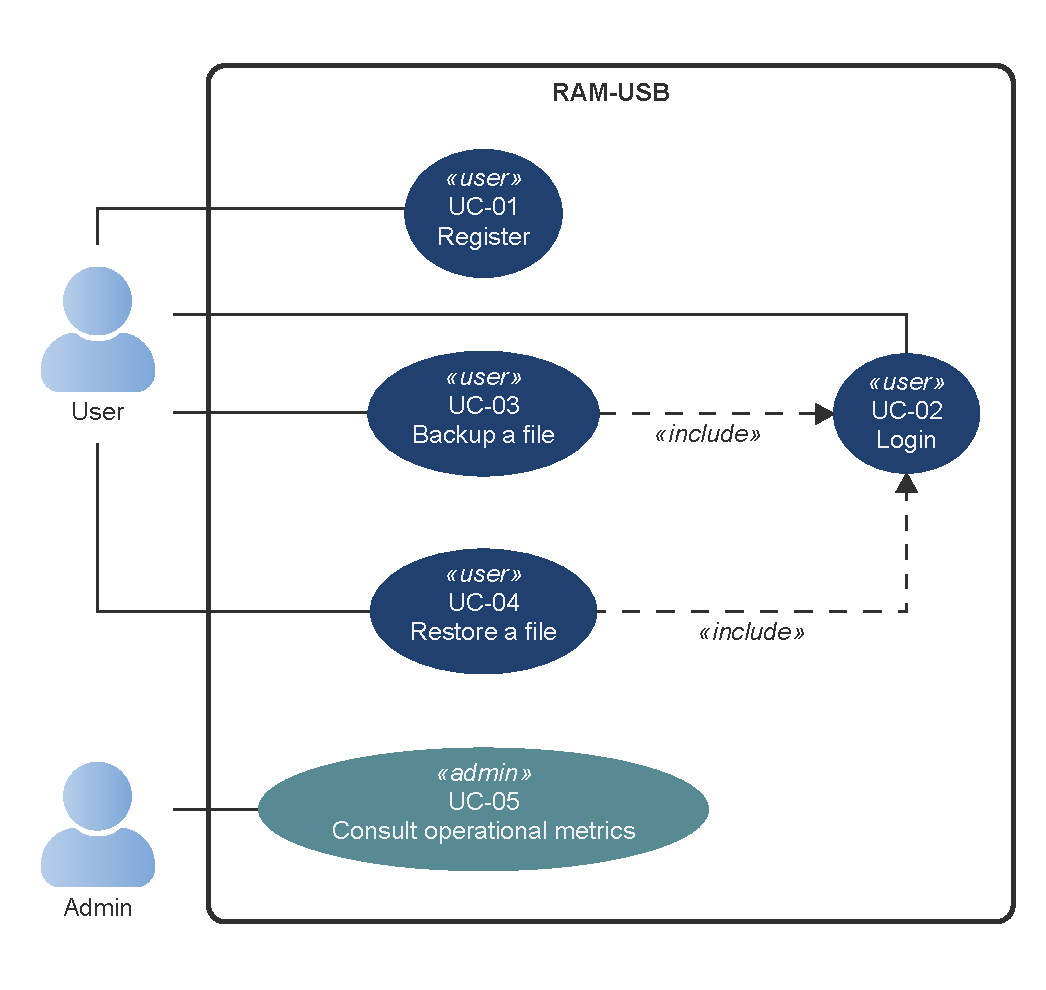
\includegraphics[width=0.5\textwidth]{figures/00-usecases-overview.pdf}
    \caption{Use case diagram of RAM-USB's main use cases.}
    \label{fig:usecases-overview}
\end{figure}

The following chapters describe how the architecture of the system realizes these use cases:
\autoref{chap:architettura} introduces the overall structure of the components and the security boundaries between
them, while Chapters 5--8 examine each functional domain in detail.

\chapter{Overall architecture and trust zones}
\label{chap:architettura}

\section{Architecture overview}

RAM-USB is an n-tier microservice architecture in which each component has a specific responsibility.
This separation reduces the risk that the compromise of one component spreads to the entire system.

The architecture of RAM-USB consists of ten
components, organized into four functional groups:
\begin{itemize}
    \item \textbf{Access and registration}: Entry-Hub, Security-Switch, Database-Vault.
    \item \textbf{Backup and restore}: Storage-Service.
    \item \textbf{Observability}: Mosquitto, Metrics-Collector, Grafana.
    \item \textbf{Network and certificates}: Network-Manager, Headscale, Certificate-Authority.
\end{itemize}

\subsection{Entry-Hub}

Entry-Hub is the public gateway of the system, that is, the component exposed to anyone on the internet. For this reason
the system grants it no implicit trust. Its process therefore runs in a distroless container
\cite{distroless-github}, following the principle of attack surface reduction recommended by
NIST SP 800-190 \cite{nist-sp-800-190}.
Indeed, without a shell, most of the known critical vulnerabilities in containers cannot be exploited
\cite{wager2024distroless}.

Entry-Hub exposes three HTTPS endpoints: \texttt{GET /api/health} and \texttt{POST /api/users} are
reachable by anyone on the internet, with a certificate signed by the public CA Let's Encrypt
\cite{aas2019letsencrypt}. \texttt{POST /api/login} uses the same certificate, but has a separate listener,
reachable only by users with access to the private network, described in detail in
\autoref{chap:rete}.

When it receives a request, Entry-Hub validates the JSON body in two phases: during decoding, it enforces a
size limit and rejects any unexpected field in the payload; then it validates the individual
email and password fields and, only during registration, the SSH key \cite{ramusb-code-eh-f-04}. If any of
these checks fails, it responds with HTTP 400 without specifying what the problem is and without forwarding the
request to the inner layers of the system. If validation succeeds, it forwards the request to
Security-Switch over mutual TLS (mTLS), verifying that the received certificate really belongs to a Security-Switch.
It waits for the Security-Switch's response and relays it to the client.

\subsection{Security-Switch}

Security-Switch exists to keep the responsibility for contacting Database-Vault and Network-Manager
out of the hands of the system's entry point: it receives incoming requests only from Entry-Hub,
authenticated via mTLS, revalidates them independently, and contacts the internal services.
The validation, error handling, and logging logic is reused by all the main services
and lives in shared internal libraries \cite{ramusb-pkg}.

The purpose of the revalidation is to apply the defense-in-depth principle \cite{nist-sp-800-53r5}.

If validation succeeds, it forwards the request to Database-Vault via mTLS.

In the case of a registration request, it asks Network-Manager to create the new user's identity
on the mesh network and the credential (pre-auth key) with which the user's device will be able to join it.

In the case of a login request, it asks Network-Manager to grant that user twelve-hour temporary access
to Storage-Service. Only once the user has obtained access to Storage-Service
will they be able to contact it and manage their own backups.

\subsection{Database-Vault}
Database-Vault is the component responsible for storing user credentials in a
PostgreSQL database. It is the only one able to access the database, but it nevertheless has no access to user files,
which are persisted on Storage-Service. This separation limits the impact of the
compromise of a single component.

The Entity-Relationship diagram is shown in \autoref{fig:er-database-vault}.
Since the database must contain only user data and there is no meaningful relationship to
store, the ER diagram is rather simple.

\begin{figure}[H]
    \centering
    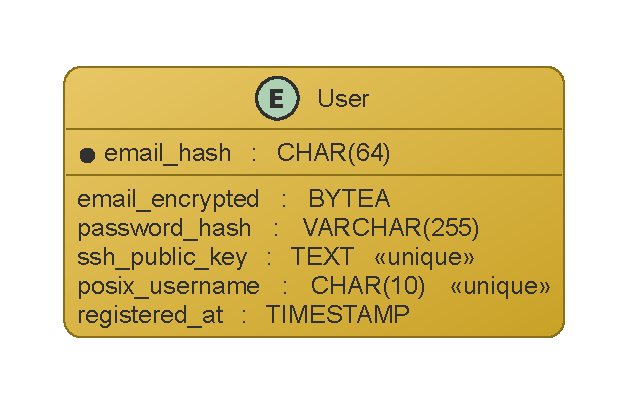
\includegraphics[width=0.35\textwidth]{figures/06-data-er-database-vault.pdf}
    \caption{Entity-Relationship diagram of the user record in Database-Vault.}
    \label{fig:er-database-vault}
\end{figure}

The email is encrypted, recoverable only with the master key, while the password is never recoverable, since
it is stored only in hashed form, as an Argon2id digest. Theft of, or unauthorized access to, the
database is therefore not enough to read either of them.

When a new user registers, after revalidating the input, Database-Vault attempts
to save the data in an atomic transaction, rejecting the request if the email or the SSH key is already
registered, but without specifying which of the two is wrong.
If the save succeeds, it asks Storage-Service to create the user's POSIX space.
If Storage-Service fails, it deletes the record just created; otherwise it informs
Security-Switch that the registration succeeded.

At login, it recomputes the hash of the received password and compares it with the stored one, then responds to
Security-Switch.

A nonexistent email and a wrong password produce the same response: in this way,
whoever attempts to log in cannot use it to discover which emails are registered.
\autoref{chap:sicurezza}, however, explains how an external user can try to determine whether
an email is already registered in the system, and also how a malicious administrator can obtain a
user's access credentials.


\subsection{Storage-Service}

Storage-Service hosts the users' backup files.
It never processes content in plaintext because, by design, it is not able to. Indeed, it receives only
files that have been deduplicated, compressed, and encrypted client-side with Restic \cite{restic-github}.

At Database-Vault's request, it creates a dedicated POSIX user, with neither an interactive shell nor a traditional
home directory. Each user instead has a writable space in their own subdirectory inside a chroot.
The filesystem structure is shown in \autoref{fig:filesystem-storage}.

\begin{figure}[H]
    \centering
    \begin{minipage}{0.85\linewidth}
    \dirtree{%
    .1 /storage/\DTcomment{root of all registered users}.
    .2 user\textless{}xxxxxx\textgreater{}/\DTcomment{owner \texttt{root:root}, permissions 0711}.
    .3 data/\DTcomment{owner \texttt{user\textless{}xxxxxx\textgreater{}}, permissions 0700}.
    }
    \end{minipage}
    \caption{Storage-Service filesystem structure, from \texttt{creator.go} and \texttt{dirmaker.go}
    \cite{ramusb-code-posixuser-owners,ramusb-code-posixuser-modes}.}
    \label{fig:filesystem-storage}
\end{figure}

Access to Storage-Service can only take place via the Secure Shell File Transfer Protocol (SFTP) \cite{sftp-filexfer},
with the SSH public key sent by the user during registration. Therefore neither
username and password authentication nor any other form of Secure Shell access outside SFTP is permitted.

On every connection, a dedicated \texttt{AuthorizedKeysCommand} binary queries Database-Vault to
obtain the user's current public key.
Any error in that call denies the connection, according to the fail-secure principle \cite{owasp-fail-securely}.

\subsection{Network-Manager}

Network-Manager is the administrator of the network rules. It is responsible for defining, modifying, and deleting the
rules that allow a user of the private mesh network to reach the other members.

During registration, it creates a dedicated Headscale user and the pre-auth key with which the user's
device will join the network.

During login, it assigns the user's node the Access Control List (ACL) tag that enables twelve-hour
temporary access to Storage-Service.
A periodic process checks expiries and removes the tag from expired nodes.

\subsection{Certificate-Authority}

Certificate-Authority is the system's private CA, based on \texttt{smallstep/certificates}
\cite{smallstep-certificates-github}.

It issues, renews, and revokes the mTLS certificates of every internal service, which makes it a
particularly critical component of the system, as well as the only one reachable by all internal services:
a malicious actor who managed to compromise it could issue forged certificates
for any organization.

Each service obtains its first certificate by contacting the CA using a bootstrap token distributed
manually by an operator out-of-band. A detailed explanation can be found in \autoref{sec:pki}.


\subsection{Headscale}

Headscale is a self-hosted implementation of the Tailscale control server \cite{headscale-github}.

It acts as the coordinator of the private mesh network: on every connection attempt between two nodes,
it enforces the reachability rules decided by Network-Manager. It also distributes, through
MagicDNS, the hostnames with which nodes resolve one another, allowing the client to locate
Storage-Service without knowing its IP address.

It also validates the pre-auth key of a new device at the moment it joins the mesh.

Unlike every other internal component except Entry-Hub, Headscale does not reside in the
private network but is reachable by anyone on the internet. \autoref{sec:paradosso-coordinatore} explores the reasons in depth.

\subsection{Mosquitto}

Mosquitto is the MQTT broker to which every service, once a minute, publishes its own operational metrics.

It enforces an ACL under which each service can write to its own topic, without ever being able to read from it,
while Metrics-Collector can only read the entire \texttt{metrics/\#} space, without ever writing to it.

\subsection{Metrics-Collector}

Metrics-Collector is the component that receives, validates, and persists the operational metrics
published by every service.

It discards every received metric whose \texttt{service} field does not match the topic it arrives from, and
persists the accepted metrics as a hypertable in TimescaleDB \cite{timescaledb-github}, with a retention of
thirty days and compression after seven days.

\subsection{Grafana}

Grafana is the visualization platform with which an administrator consults the health status and the
performance of the system \cite{grafana-github}.

It reads from TimescaleDB directly, without going through Metrics-Collector.
The Grafana dashboard shows response times, throughput, and active connections.
\autoref{chap:osservabilita} covers this observability pipeline in detail.

\clearpage

\autoref{fig:architecture-container} summarizes the architecture just described together with the
communication protocols used.

\begin{figure}[H]
    \centering
    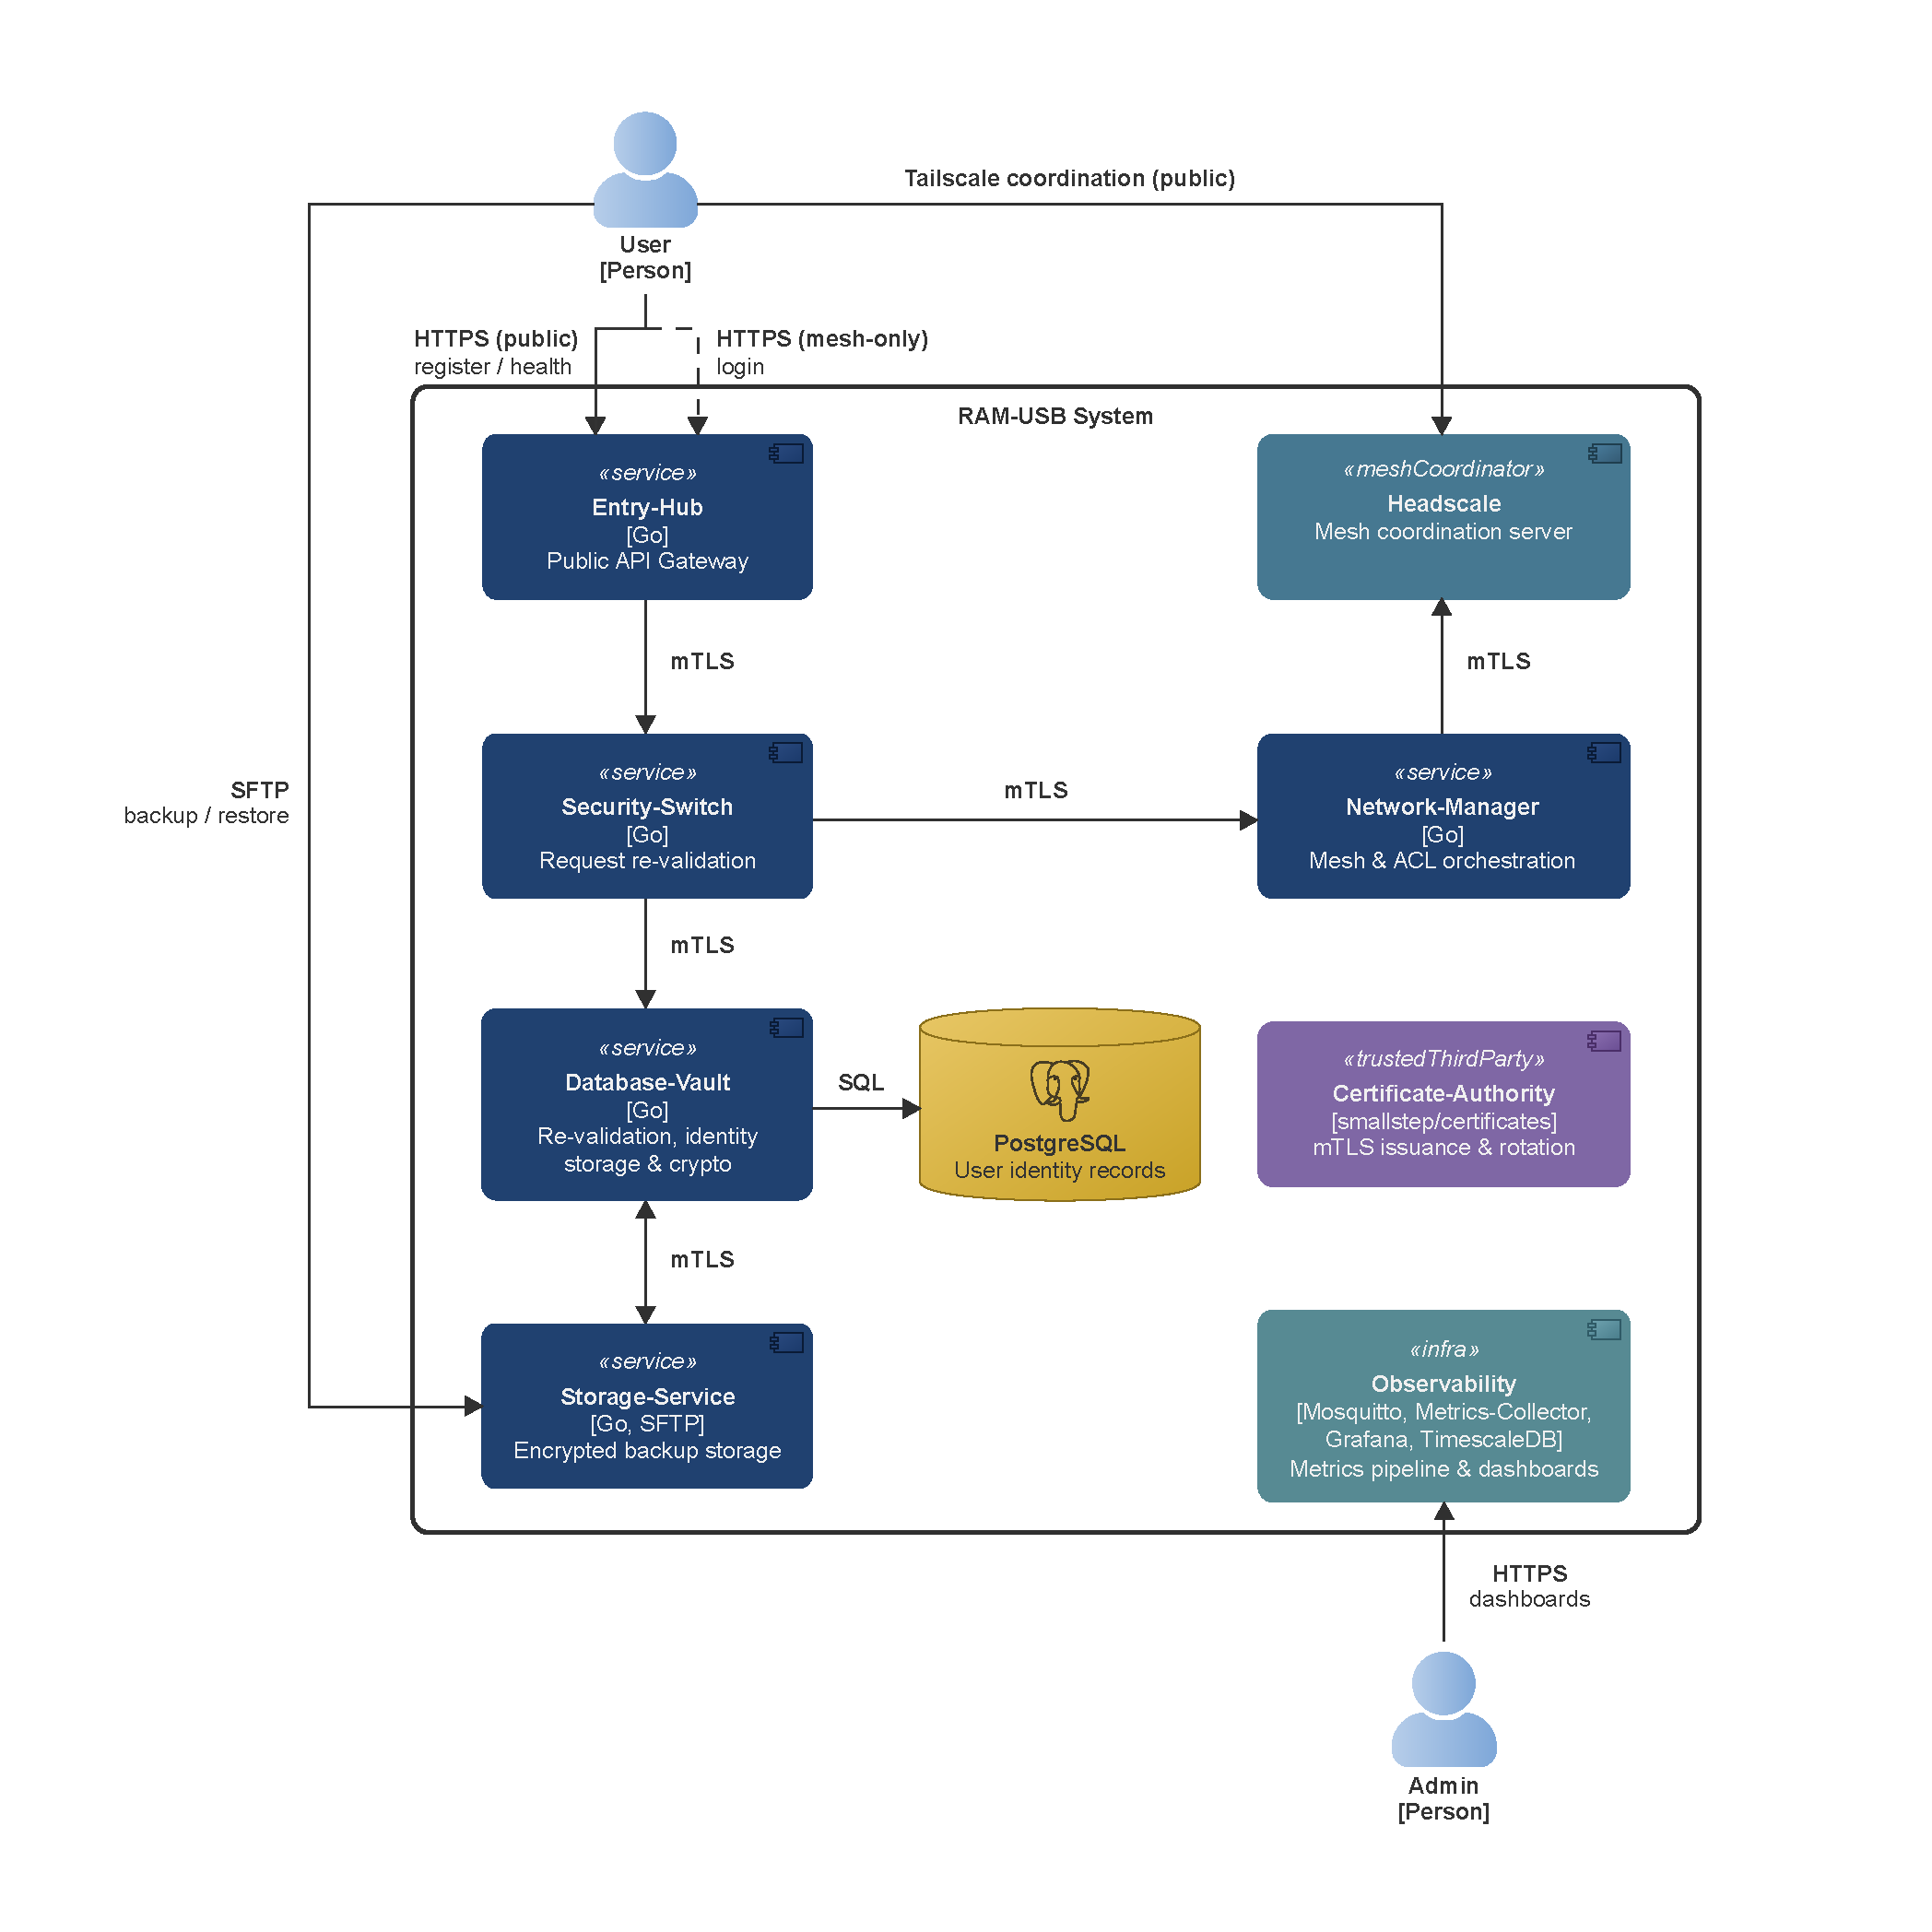
\includegraphics[width=0.8\textwidth]{figures/01-architecture-container.pdf}
    \caption{Container diagram of RAM-USB.}
    \label{fig:architecture-container}
\end{figure}

\section{Inter-service communication model}

Each service exposes its own HTTPS API built on Go's standard library, \texttt{net/http}.
Requests and responses are JSON bodies, and each endpoint is registered on a minimal router,
\texttt{http.ServeMux}. The minimum allowed TLS version is 1.3.

The endpoints listed here follow REST conventions \cite{fielding2000rest}.
\begin{itemize}
    \item \texttt{GET /api/health}, \texttt{POST /api/users} on Entry-Hub,
    \item \texttt{GET /internal/v1/public-key/\symbol{123}posix\_username\symbol{125}} on Database-Vault,
    \item \texttt{POST /internal/v1/posix-users} on Storage-Service, and
    \item \texttt{POST /internal/v1/mesh-users}, \texttt{POST /internal/v1/grants} on Network-Manager
\end{itemize}

\texttt{POST /api/login} is the only exception, because a successful login returns only the confirmation that
an action took place, with no identifier that a real \texttt{sessions} resource would require in order to
be read with GET or deleted with DELETE. The twelve-hour ACL token that the login grants remains
internal to Network-Manager and expires on its own.

The publication of metrics, moreover, is asynchronous: each service publishes its own messages on
a dedicated Message Queuing Telemetry Transport (MQTT) topic without any need to wait for a response.

This system structure comes at a significant cost: every registration and login passes through
four distinct processes, each with its own mTLS handshake and its own revalidation.
Latency is therefore much higher than in a monolithic system, and, should it ever need to be reduced, it cannot be
reduced by skipping one of the steps. Moreover, the service remains available to users only as long as
the seven components that take part in a request's path remain available, while the
observability chain can go down without the user noticing.

The two costs, however, are not of the same kind. Latency is inherent to the design and accepted together
with the architecture; availability, by contrast, is a deployment problem, and
\autoref{chap:deployment} discusses to what extent the underlying infrastructure is able to mitigate it.

\section{Trust zones and security boundaries}
\label{sec:trust-zones}

\autoref{fig:trust-zones} shows the reachability rules that Network-Manager applies to the mesh network.

The two outermost zones belong to the user, before and after authentication. A user who is registered but
not yet authenticated, and who therefore belongs to the \emph{Unauthenticated User Zone}, sees and can contact
only Entry-Hub. After login, the same node enters the \emph{Authenticated User Zone} and obtains
temporary reachability to Storage-Service.

Certificate-Authority reaches only the MQTT broker, but is reached by every other
internal component, to allow it to renew its own X.509 certificate.

The fourth zone, the \emph{Public Zone}, contains only Headscale, reachable from the public
network. \autoref{sec:paradosso-coordinatore} explains the reason in detail. However,
Network-Manager's calls to Headscale are still protected by mTLS authentication and
by the Headscale API key.

\begin{figure}[H]
    \centering
    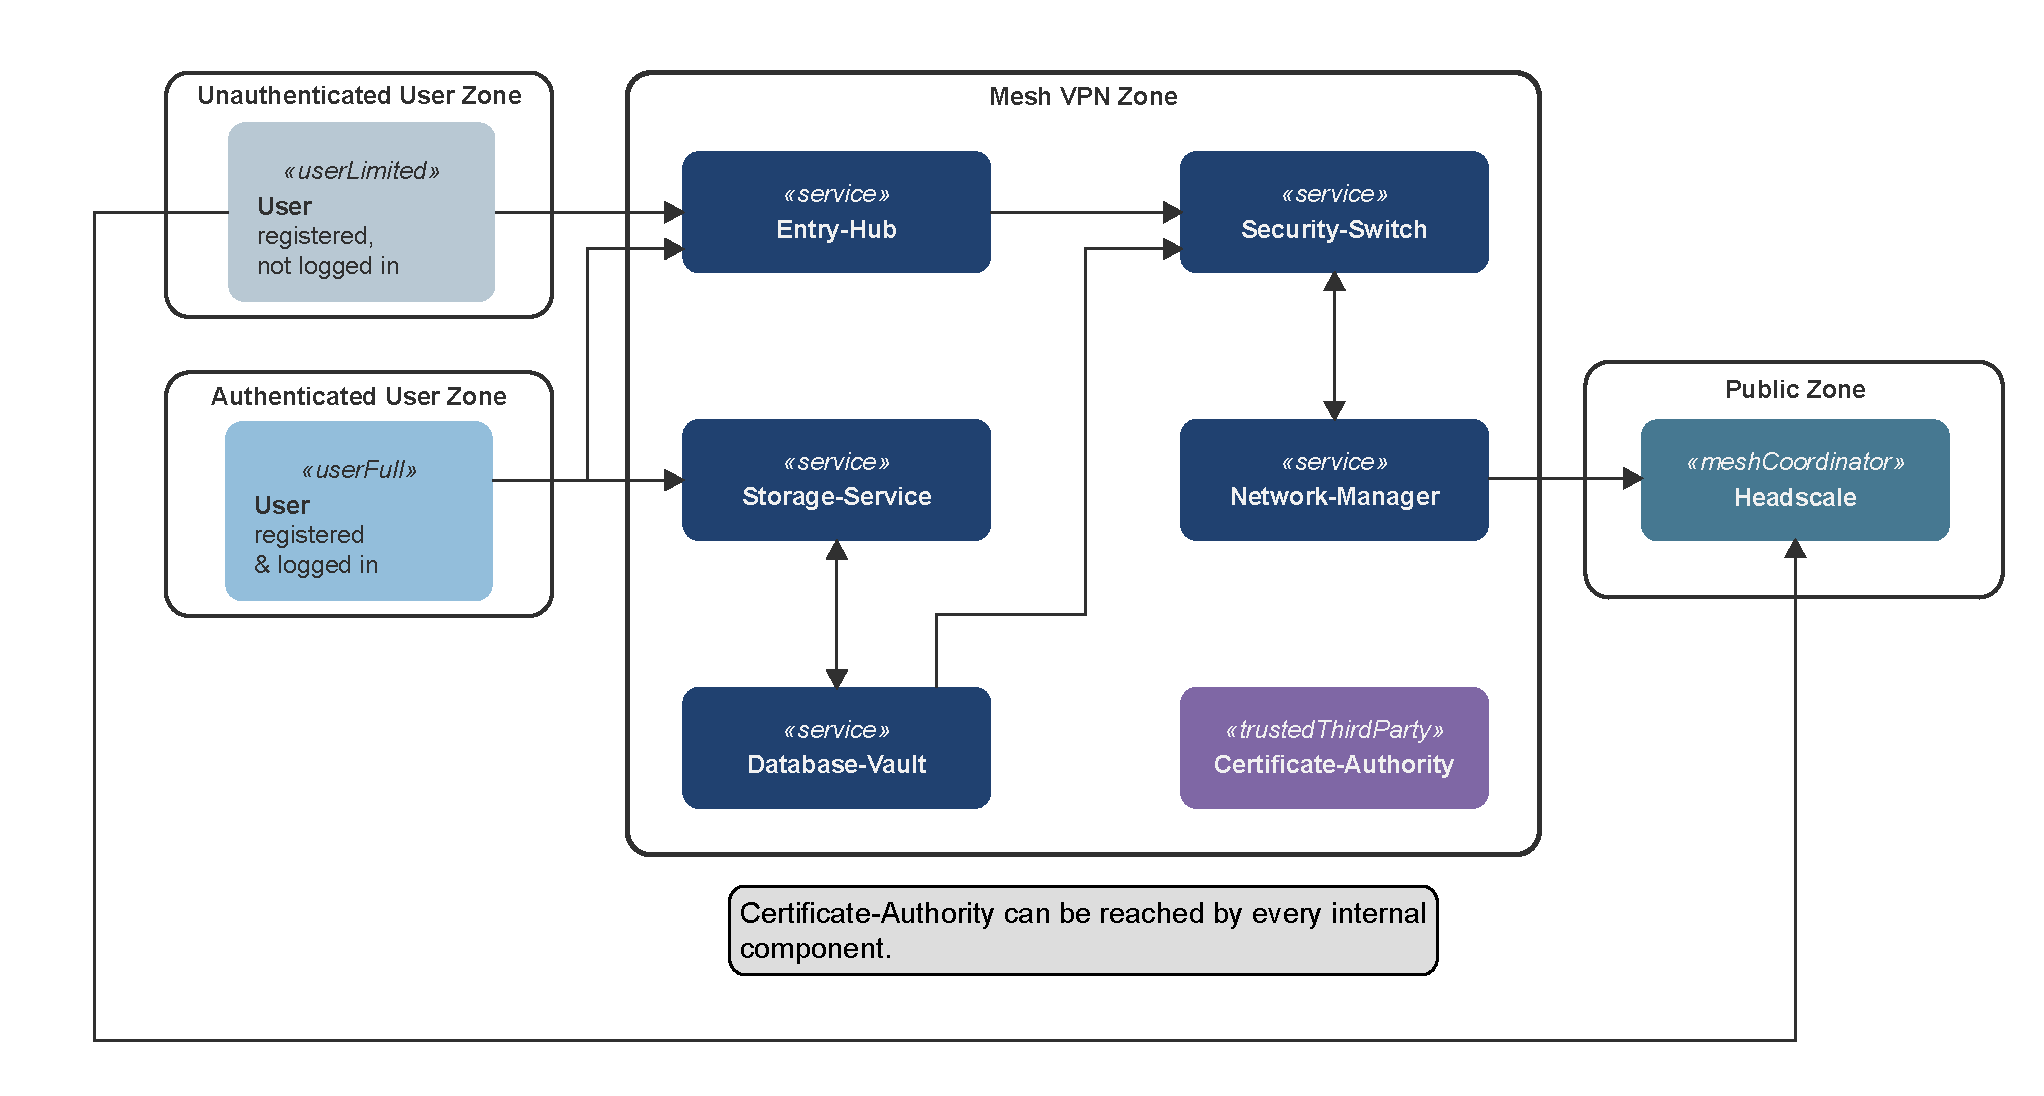
\includegraphics[width=0.8\textwidth]{figures/09-security-trust-zones.pdf}
    \caption{Trust zones and reachability on the mesh network.}
    \label{fig:trust-zones}
\end{figure}

\section{PKI and certificate management}
\label{sec:pki}

RAM-USB uses two certificate authorities, as illustrated in \autoref{fig:pki-hierarchy}.

Let's Encrypt, a public CA, signs only the certificate that Entry-Hub presents on its public
endpoints. This is because the certificate must be verifiable by an external client that does not yet have access
to the system's internal network. A certificate signed by RAM-USB's private Certificate-Authority would not
be trusted.

Every other communication instead uses the private Certificate-Authority, based on
\texttt{smallstep/\allowbreak certificates}.

Every private certificate follows the same bootstrap scheme: each service receives,
out-of-band and only once, a single-use bootstrap token, and presents it to Certificate-Authority
in exchange for its own initial certificate. Subsequent renewals present the mTLS certificate
already held. The token remains a throwaway secret and therefore does not need to be protected once
consumed.

A valid X.509 certificate only proves that Certificate-Authority approved that client, not that it is
the client expected for that connection. For this reason each service also verifies the
\texttt{organization} field of the certificate.

\begin{figure}[h]
    \centering
    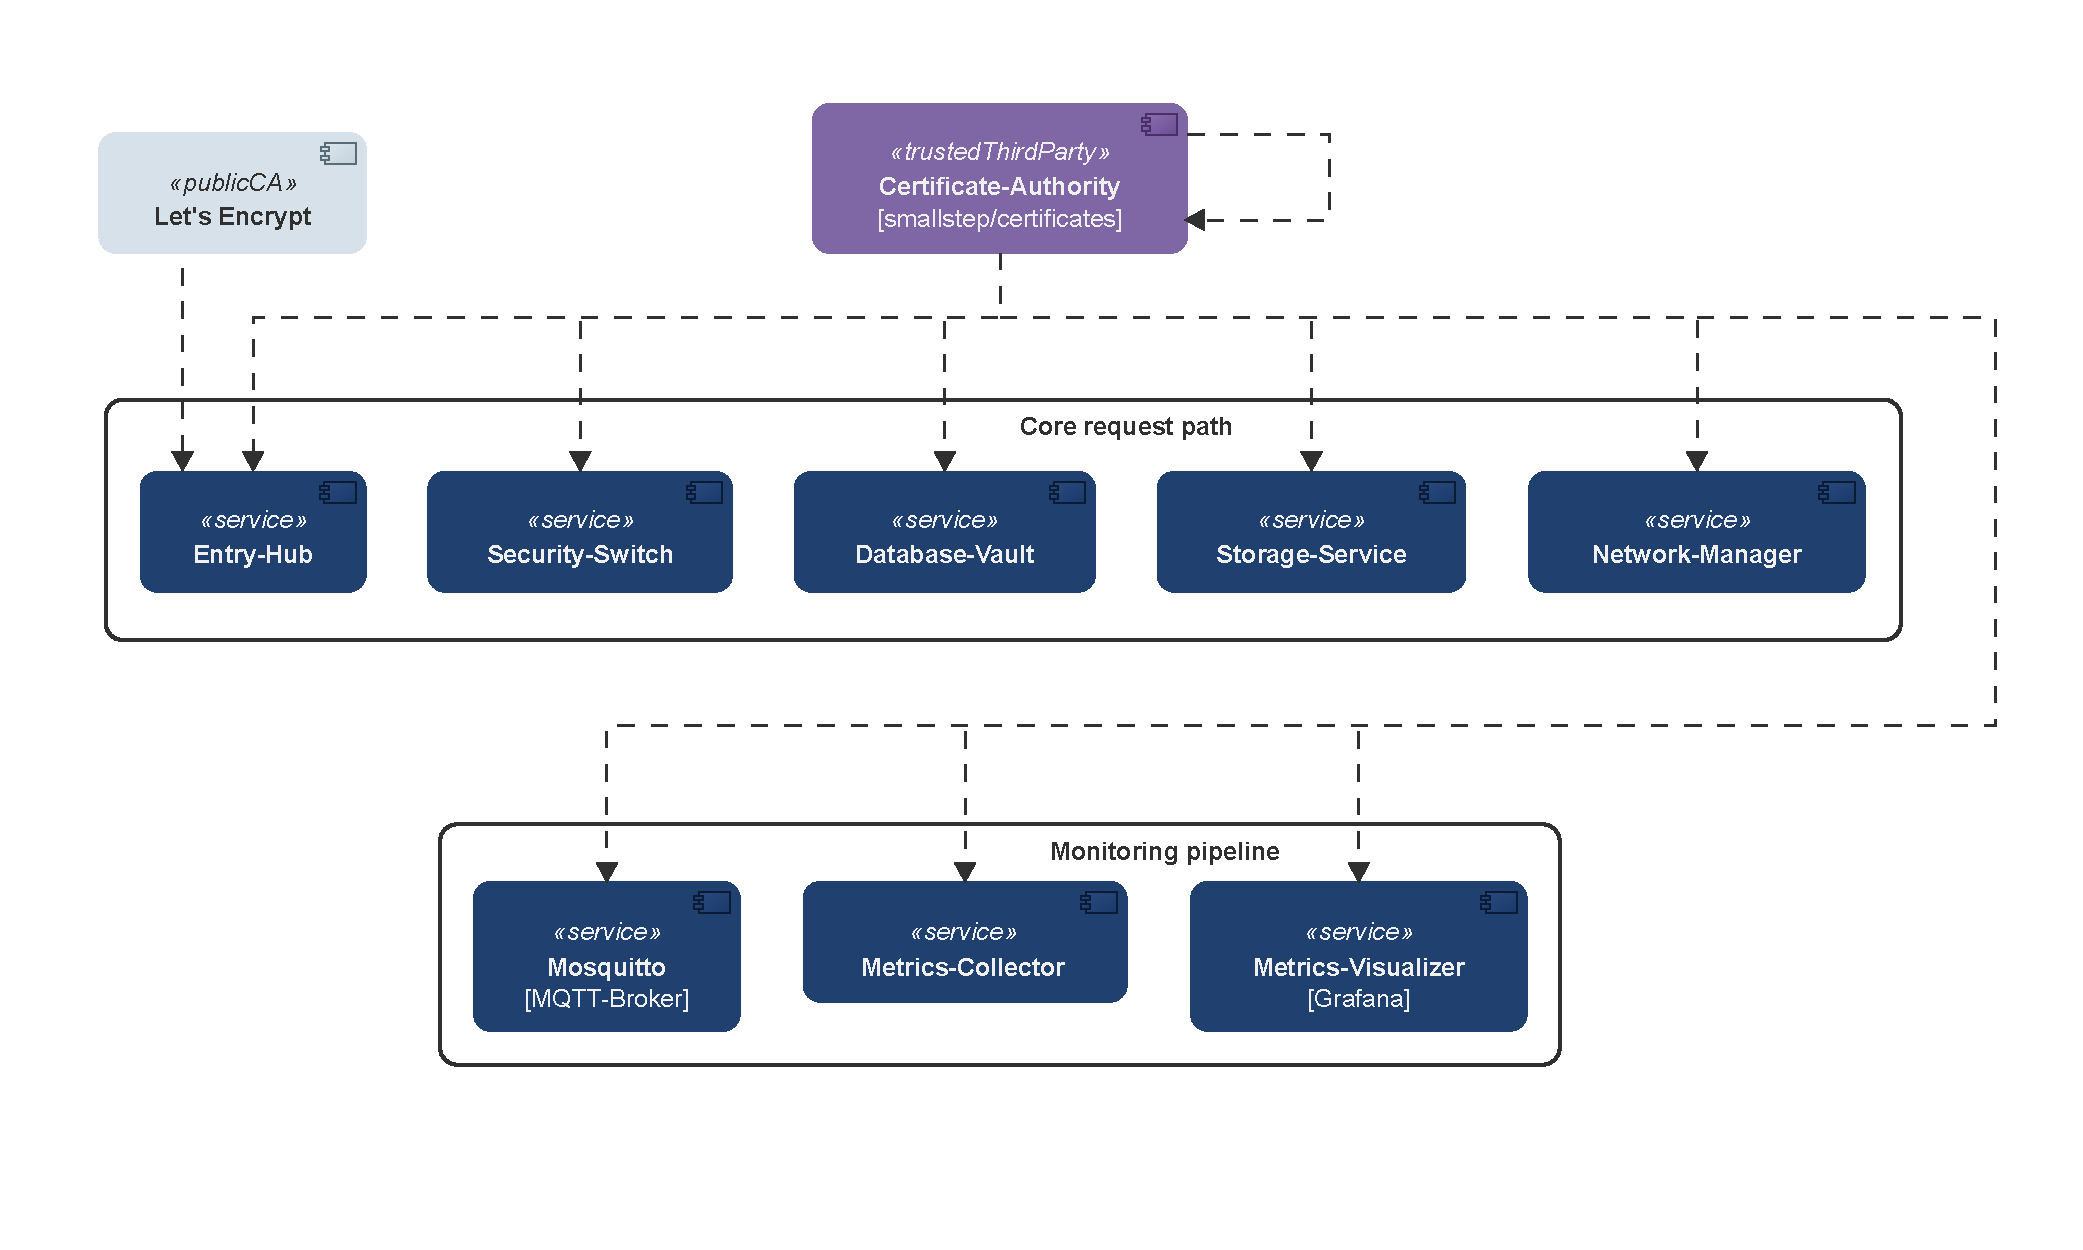
\includegraphics[width=\textwidth]{figures/08-security-pki-hierarchy.pdf}
    \caption{Hierarchy of the certificate authorities and signing relationships.}
    \label{fig:pki-hierarchy}
\end{figure}


\chapter{Authentication and identity management}
\label{chap:autenticazione}

\section{Request lifecycle}
\label{sec:ciclo-richiesta}

A registration or login request passes through three services before becoming a record:
Entry-Hub, Security-Switch, and Database-Vault. All three apply the same checks to the input,
each one independently of the others.

Validation takes place in two phases. The first concerns the request body: the payload is
read up to a limit of 2048 bytes and rejected if it exceeds it, and the JSON decoder rejects any unexpected field.

The second phase concerns the individual fields \cite{ramusb-code-eh-f-04}. The email must be a
single, syntactically valid address according to RFC 5322 \cite{rfc5322}; the password must be
between 8 and 128 characters long and use at least three categories among lowercase letters, uppercase letters, digits, and symbols.
At registration, moreover, the SSH public key must be well formed.

If a check fails, the response is HTTP 400 without indicating which check did not pass, the
log records the problem without identifying the user, and the request does not proceed inward.
The message stays generic because a detailed error would help an attacker more than it helps a
user acting in good faith, whose own client has already applied the same checks.

The three services share the same validation library, so repeating the check does not
introduce algorithmic diversity, but it guarantees that no service takes for granted that the
previous one did its job. In this way, if, for example, a tampered request coming from a
compromised service were to reach Database-Vault, the validation would still be performed and would cause the request to be discarded.

Finally, internal errors are translated into HTTP status codes. \autoref{tab:codici-http} summarizes the codes
that reach the user, attributing each code to the service that emits it.

Entry-Hub builds only the errors that originate in itself: a failed validation and a
call to Security-Switch that went wrong. Everything else it relays back to the client exactly as it arrives
from the inside, without modifying it. For this reason, a 401 or a 409 reaches the user despite never
being produced by Entry-Hub.

\begin{table}[H]
\centering
\caption{HTTP status codes returned to the client and their meaning in the system.}
\label{tab:codici-http}
\begin{tabular}{@{}l p{\dimexpr0.58\linewidth\relax} l@{}}
\hline
\textbf{Code} & \textbf{Meaning} & \textbf{Issued by} \\
\hline
400 & Validation failed, without indicating which check did not pass & both \\
401 & Invalid credentials, does not specify whether nonexistent email or wrong password & Security-Switch \\
403 & Explicit refusal from Network-Manager & Security-Switch \\
409 & Email or SSH key already registered, does not specify which of the two & Security-Switch \\
500 & Internal error not otherwise classified & both \\
502 & Downstream service unreachable or returning an unexpected response & both \\
503 & Call to Security-Switch timed out & Entry-Hub \\
504 & Call to Database-Vault or Network-Manager timed out & Security-Switch \\
\hline
\end{tabular}
\end{table}

The codes that the two services build on their own differ in two respects:
the first is 403, which only Security-Switch can emit, because it is the only one of the two that can receive an
explicit refusal from an internal service. The second concerns timed-out calls: Entry-Hub responds 503,
Security-Switch 504.

In all cases, the response body is sanitized and the error details remain in the internal
logs.

\section{Credential encryption and hashing}

Database-Vault treats the data it receives in three different ways:

\begin{itemize}
    \item the SSH key is public, so it does not require secrecy;
    \item the email is at the same time a lookup key and personal data to be protected, but it must also be
		recoverable when needed;
    \item the password must not be recoverable, not even by whoever administers the database.
\end{itemize}

The email is normalized to lowercase and reduced to its SHA-256 digest, which becomes the primary key
of the record. Normalization guarantees that the same address written with different letter case at login
produces the same key as at registration.
This hash is deterministic by necessity, because it must enable the lookup. The fundamental limitation of
this approach, together with its mitigation, is discussed in \autoref{chap:sicurezza}.

Alongside the digest that acts as the lookup key, the record keeps an encrypted copy of the email,
so that the address remains recoverable.
From a master key and a random 16-byte salt, generated for that record,
a dedicated key is derived with HKDF-SHA256 \cite{rfc5869}, with which the email is encrypted with
AES-256-GCM \cite{nist-sp-800-38d} using a random 12-byte nonce. Salt, nonce, and ciphertext
are stored in the record, while the derived key is zeroed as soon as the cipher has consumed it.
Deriving a key for each record, instead of encrypting everything with the master key, reduces the amount
of data protected by a single key.

\Needspace{22\baselineskip}
\begin{lstlisting}[caption={Per-record key derivation in \texttt{newGCM}, from
\texttt{encryption.go} \cite{ramusb-code-hkdf-newgcm}.}, label={lst:hkdf}]
func newGCM(masterKey, salt []byte) (cipher.AEAD, error) {
	derivedKey := make([]byte, derivedKeySize)
	kdf := hkdf.New(sha256.New, masterKey, salt, []byte(hkdfInfo))
	if _, err := io.ReadFull(kdf, derivedKey); err != nil {
		return nil, fmt.Errorf("encryption: derive key: %w", err)
	}

	block, err := aes.NewCipher(derivedKey)
	for i := range derivedKey {
		derivedKey[i] = 0
	}
	if err != nil {
		return nil, fmt.Errorf("encryption: new AES cipher: %w", err)
	}

	gcm, err := cipher.NewGCM(block)
	if err != nil {
		return nil, fmt.Errorf("encryption: new GCM: %w", err)
	}

	return gcm, nil
}
\end{lstlisting}


The password, instead, is concatenated with a pepper, read from an environment variable, and passed to Argon2id
\cite{rfc9106} together with a random 16-byte salt generated on the spot for that record.

OWASP \cite{owasp-password-storage} proposes several configurations equivalent to one another, which
trade memory for number of passes. RAM-USB starts from the one with the most memory and doubles its
passes, thus paying at each verification twice the work that OWASP considers sufficient. It is a
cost that makes recovering the passwords from a stolen database impractical. The pepper further complicates
an offline attack: unlike the salt, which is stored in the record and only prevents
a single guess from applying to several users at once, the pepper does not appear in the database. Without the pepper,
no guess is computationally feasible, and a copy of the database is therefore not
sufficient to carry out the attack.

The result is stored as a self-describing string in PHC format, the encoding convention
that originated from the Password Hashing Competition. Each record therefore carries with it the parameters with which it was created,
and verification at login uses them in place of the service's current constants.
In this way, changing the parameters for new users does not invalidate already existing records.

\autoref{tab:phc} lists the fields of that string, in the order in which they appear in the record.

\begin{table}[H]
\centering
\caption{Fields of the PHC string in which Database-Vault stores the password hash.}
\label{tab:phc}
\begin{tabular}{@{}l p{\dimexpr0.70\linewidth\relax}@{}}
\hline
\textbf{Field} & \textbf{Meaning} \\
\hline
\texttt{argon2id} & Algorithm variant \\
\texttt{v=19} & Argon2 version: the byte \texttt{0x13} fixed by RFC 9106, printed in decimal \\
\texttt{m=47104} & Working memory in KiB, i.e.\ 46 MiB \\
\texttt{t=2} & Number of passes over memory \\
\texttt{p=1} & Degree of parallelism \\
salt & Random 16-byte salt, generated for that record \\
digest & 32-byte hash produced by Argon2id \\
\hline
\end{tabular}
\end{table}

The master key and the pepper both reside in environment variables, with no backup or
rotation procedure. The risk is discussed in \autoref{chap:conclusioni}.


\autoref{sch:credenziali} summarizes the transformations just described, with the following symbols:

\begin{itemize}
    \item $e$: the received email;
    \item $p$: the received password;
    \item $k_{SSH}$: the SSH public key;
    \item $\pi$: the pepper;
    \item $MK$: the master key;
    \item $s$, $n$, $s_p$: respectively the HKDF salt, the AES-GCM nonce, and the
    Argon2id salt, generated for that record;
    \item $\stackrel{R}{\leftarrow}$: a uniform random draw from the indicated set.
\end{itemize}

\begin{schema}
\centering
$\begin{array}{rl}
1. & s,\, s_p \stackrel{R}{\leftarrow} \{0,1\}^{128}, \quad n \stackrel{R}{\leftarrow} \{0,1\}^{96} \\[4pt]
2. & k_h = \mathrm{SHA\mbox{-}256}(\mathrm{lower}(e)) \\[4pt]
3. & k = \mathrm{HKDF\mbox{-}SHA256}(MK,\, s) \\[4pt]
4. & c = \mathrm{AES\mbox{-}GCM}_{k}(n,\, e) \\[4pt]
5. & h = \mathrm{Argon2id}(p \, \| \, \pi,\, s_p) \\[4pt]
6. & r = (k_h,\, s,\, n,\, c,\, \mathrm{PHC}(h,\, s_p),\, k_{SSH})
\end{array}$
\caption{Transformations applied to the credentials before the record is written.}
\label{sch:credenziali}
\end{schema}

\subsection{Password strength}
\label{sec:entropia}

The validation rules of \autoref{sec:ciclo-richiesta} delimit the space of admissible
passwords, and from that space one can derive, in the best case, how much uncertainty the policy can
guarantee against whoever tries to guess a password, that is, how many possibilities they must consider, not
knowing which one was chosen.

How much that uncertainty is worth, however, depends on how the password was chosen. In the best case, in
which it is produced by a pseudorandom generator drawing from the entire admissible alphabet, every
admissible password is equiprobable and the uncertainty
is therefore maximal. In the worst case, in which it is constructed by a person, some passwords are
far more probable than others; for example, \texttt{Password1!} is chosen much more often than
a random sequence of the same length. The value computed here is that of the best case, that is, an
upper bound.

In this case, then, the computation reduces to counting the distinct values that the policy admits, starting
from the cardinality of the four categories:

\[
\begin{array}{rcll}
n_1 & = & 26  & \mbox{lowercase} \\
n_2 & = & 26  & \mbox{uppercase} \\
n_3 & = & 10  & \mbox{digits} \\
n_4 & = & 33  & \mbox{symbols} \\[2pt]
N   & = & \sum_i n_i = 95 & \mbox{characters available in total}
\end{array}
\]

The constraint of at least three categories excludes the strings that use at most two of them, so to count the
valid passwords it is easier to first count those that are not valid: one starts from all $N^L$ possible
strings and subtracts those that use a single category and those that use exactly two.

The first group is immediate, because the strings written with category $i$ alone are $n_i^L$. For
the second, it is not enough to sum $(n_i + n_j)^L$ over all pairs, because that value counts the strings
written with those two alphabets only and therefore also includes those of $i$ alone and of $j$ alone:
subtracting $n_i^L$ and $n_j^L$ leaves the strings that actually use both categories. By the
inclusion-exclusion principle, the number of valid passwords of length $L$ is therefore

\[
V(L) = N^L - \sum_{i=1}^{4} n_i^L
       - \sum_{i<j} \left[ (n_i + n_j)^L - n_i^L - n_j^L \right].
\]

An attacker lacking any information must consider all $V(L)$ admissible candidates.
That number is customarily expressed in bits, that is, as an exponent of 2: $b$ bits correspond to $2^b$
candidates. If the password is drawn uniformly, the attacker's uncertainty is therefore
$\log_2 V(L)$ bits.

For the minimum admissible length, $L = 8$, one obtains $V(8) = 6.27 \cdot 10^{15}$, that is,
$\log_2 V(8) \approx 52.48$ bits.

The comparison with the unconstrained space shows how much each of the two rules weighs. Without the
category constraint, all eight-character strings over the alphabet would be admissible, namely
$N^8 = 95^8 = 6.63 \cdot 10^{15}$, that is, 52.56 bits. The category constraint therefore reduces the entropy by 0.08 bits.
Each additional character, instead, increases the entropy by $\log_2 95 \approx 6.57$ bits.

From these figures it might seem that the constraint simplifies the work of a malicious actor instead
of countering it, and this is true, albeit to a negligible extent, in the case in which passwords are created by
pseudorandom generators.
The purpose of that rule, however, is not to increase entropy, but rather to constrain the choice of
a person, who tends to stop at lowercase letters only or at letters and digits. How much it is worth in that
role cannot be derived from this computation.

Whether the two rules should coexist, or whether it would be better to replace the category constraint with a
greater minimum length, therefore remains an open question, taken up among the future work in
\autoref{chap:conclusioni}.


How well that space holds up, however, also depends on the cost of each guess, that is, on the
Argon2id parameters (\autoref{tab:phc}).

\section{Registration}

When the request reaches Database-Vault and has been revalidated, the service computes the three
transformations of the previous section and tries to write the record in a single atomic
transaction \cite{ramusb-code-saveuser}. Two uniqueness constraints protect the table, one
on the email hash and one on the SSH public key: if either of them is violated, the registration
is rejected with HTTP 409, without saying which of the two caused the conflict. That code,
however, tells an unauthenticated sender that one of the two submitted values was
already present, and whoever submits a freshly generated SSH key knows that the only other candidate is the email.
\autoref{chap:sicurezza} analyzes this problem and presents a possible mitigation.

At this point the record exists, but the user does not yet have a space in which to write.
Database-Vault then generates a POSIX username of the form
\texttt{user<xxxxxx>}, where the six digits are random characters from a
base-36 alphabet, and asks Storage-Service to create the corresponding account. How
Storage-Service creates and isolates it is the subject of \autoref{chap:storage}.

If that creation fails, the record just written is deleted. If the rollback also fails,
the service reports it with a dedicated error.

When instead both steps succeed, Database-Vault informs Security-Switch that the
registration was successful, and the latter proceeds with the orchestration described
in the concluding section of this chapter.

\Needspace{12\baselineskip}
\begin{lstlisting}[caption={Compensating rollback after a Storage-Service failure, from
\texttt{registration.go} \cite{ramusb-code-registration-rollback}.}, label={lst:rollback}]
		rollbackCtx, cancel := context.WithTimeout(context.WithoutCancel(ctx), rollbackTimeout)
		defer cancel()

		if delErr := store.DeleteUser(rollbackCtx, input.EmailHash); delErr != nil {
			return Result{
				Outcome: OutcomeFailed,
				Err:     fmt.Errorf("%w: posix creation error: %w; delete error: %w", ErrOrphanedRecord, err, delErr),
			}
		}
\end{lstlisting}

\autoref{fig:uc01} summarizes the entire sequence, from the client's request to the response. The
last two exchanges, those toward Network-Manager, are the subject of the concluding section of this
chapter.

\begin{figure}[H]
    \centering
    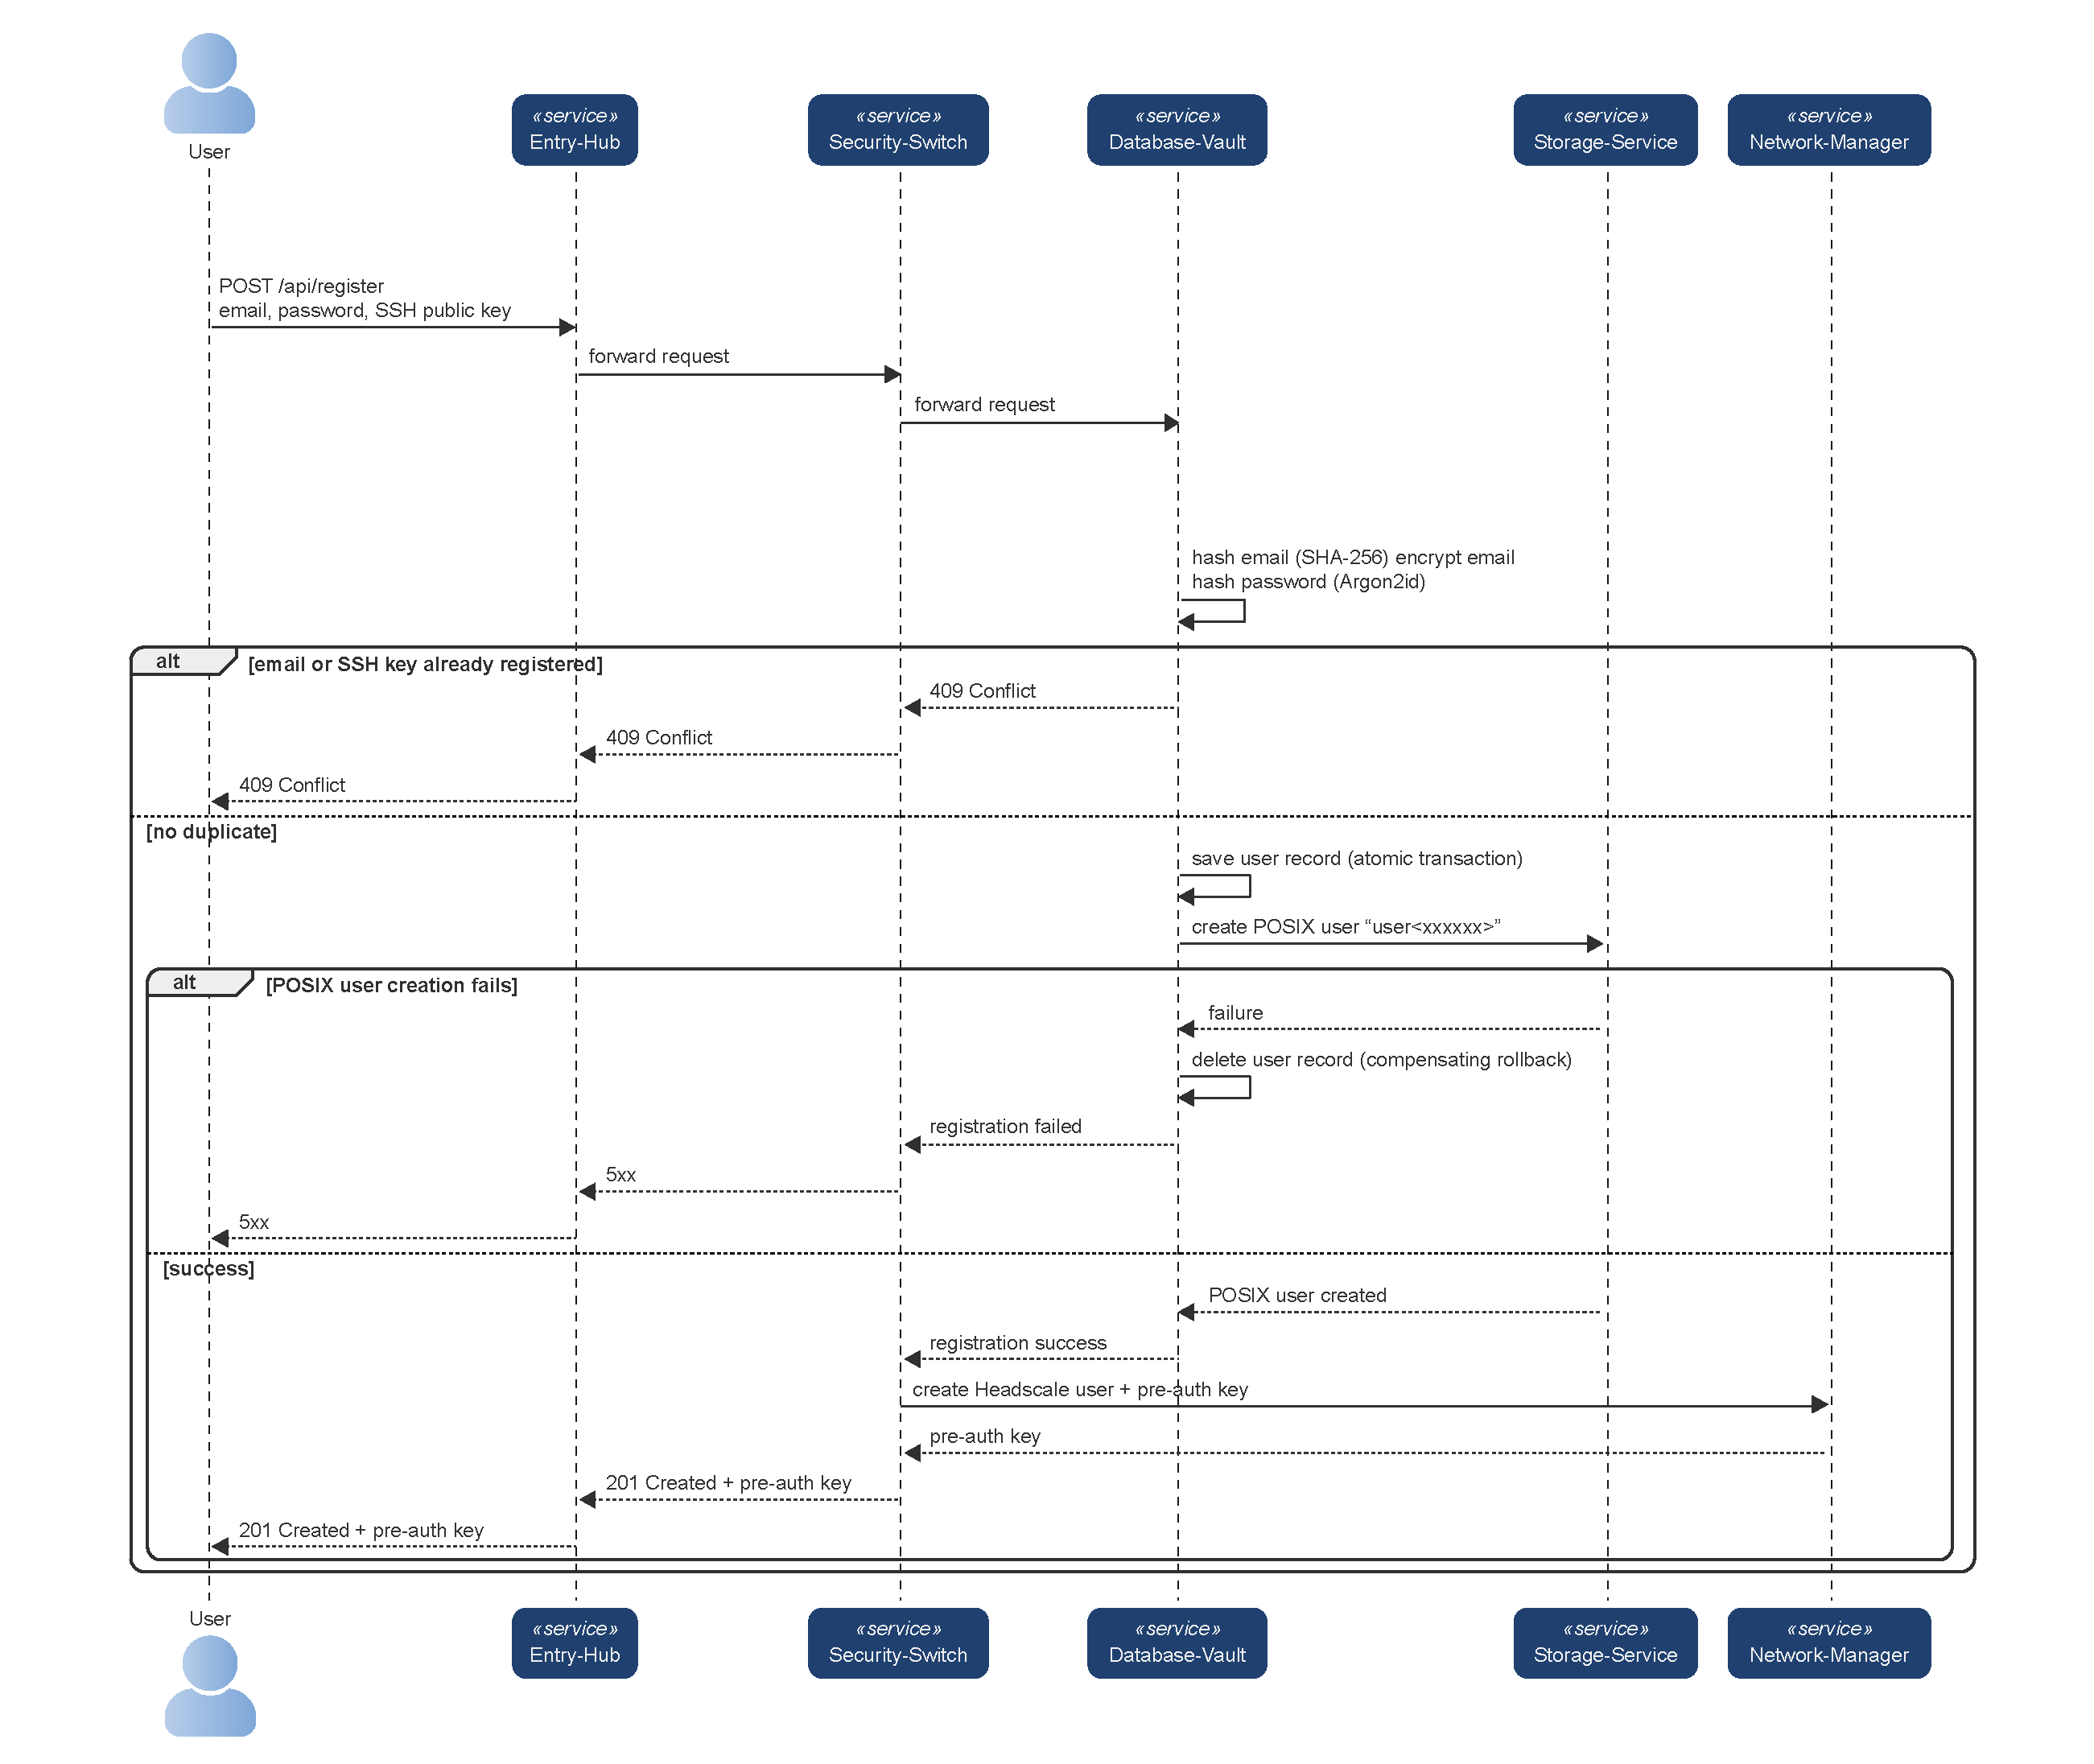
\includegraphics[width=\textwidth]{figures/03-usecases-sequence-uc01-registration.pdf}
    \caption{Registration sequence (UC-01).}
    \label{fig:uc01}
\end{figure}

\section{Login}
\label{sec:login}

During login, Database-Vault recomputes the SHA-256 digest of the received email and uses it to look up the
record.

Salt and cost parameters are extracted from the record's PHC string. Argon2id is recomputed with
those values and with the pepper, and the resulting digest is compared with the stored one through a
constant-time comparison, which therefore does not allow one to infer how many leading bytes of the two values match.

A nonexistent email and a wrong password must produce the same response, and must not
be distinguishable even in the logs. The two paths therefore converge on a single sentinel
error, and the content of the original error is discarded \cite{ramusb-code-login}.

Making the response and the log identical, however, is not enough to make the two cases indistinguishable, because
a third observable difference remains: time. Argon2id, with the parameters of the previous
section, costs tens of milliseconds, and if it were executed only when a record actually
exists, an attacker could distinguish the two situations by measuring the response latency.
The solution adopted is to spend the same time even when there is nothing to verify.

\Needspace{6\baselineskip}
\begin{lstlisting}[caption={Dummy verification used on the rejection paths, from \texttt{hash.go}
\cite{ramusb-code-verify-dummy}.}, label={lst:verifydummy}]
func VerifyDummy(password, pepper []byte) {
	_, _ = VerifyPassword(password, pepper, dummyHash())
}
\end{lstlisting}

The function recomputes Argon2id against a dummy hash, built only once per process with
the same cost parameters as the real records, and discards the result. It is called on every
rejection path, including the one in which the lookup itself fails, so that not even an infrastructure
failure becomes easily measurable from the outside.

Every uncertainty leads to the same outcome. If the verification cannot complete, for example because
the stored hash is malformed, the response remains 401, according to the
fail-secure principle \cite{owasp-fail-securely}. In the logs that case remains distinguishable, because an operator
needs to know whether it is a corrupted record, a careless user, or a genuine attack.

\autoref{fig:uc02} summarizes the complete login sequence, including the branch in which the two causes
of rejection converge on the same response.

\begin{figure}[h]
    \centering
    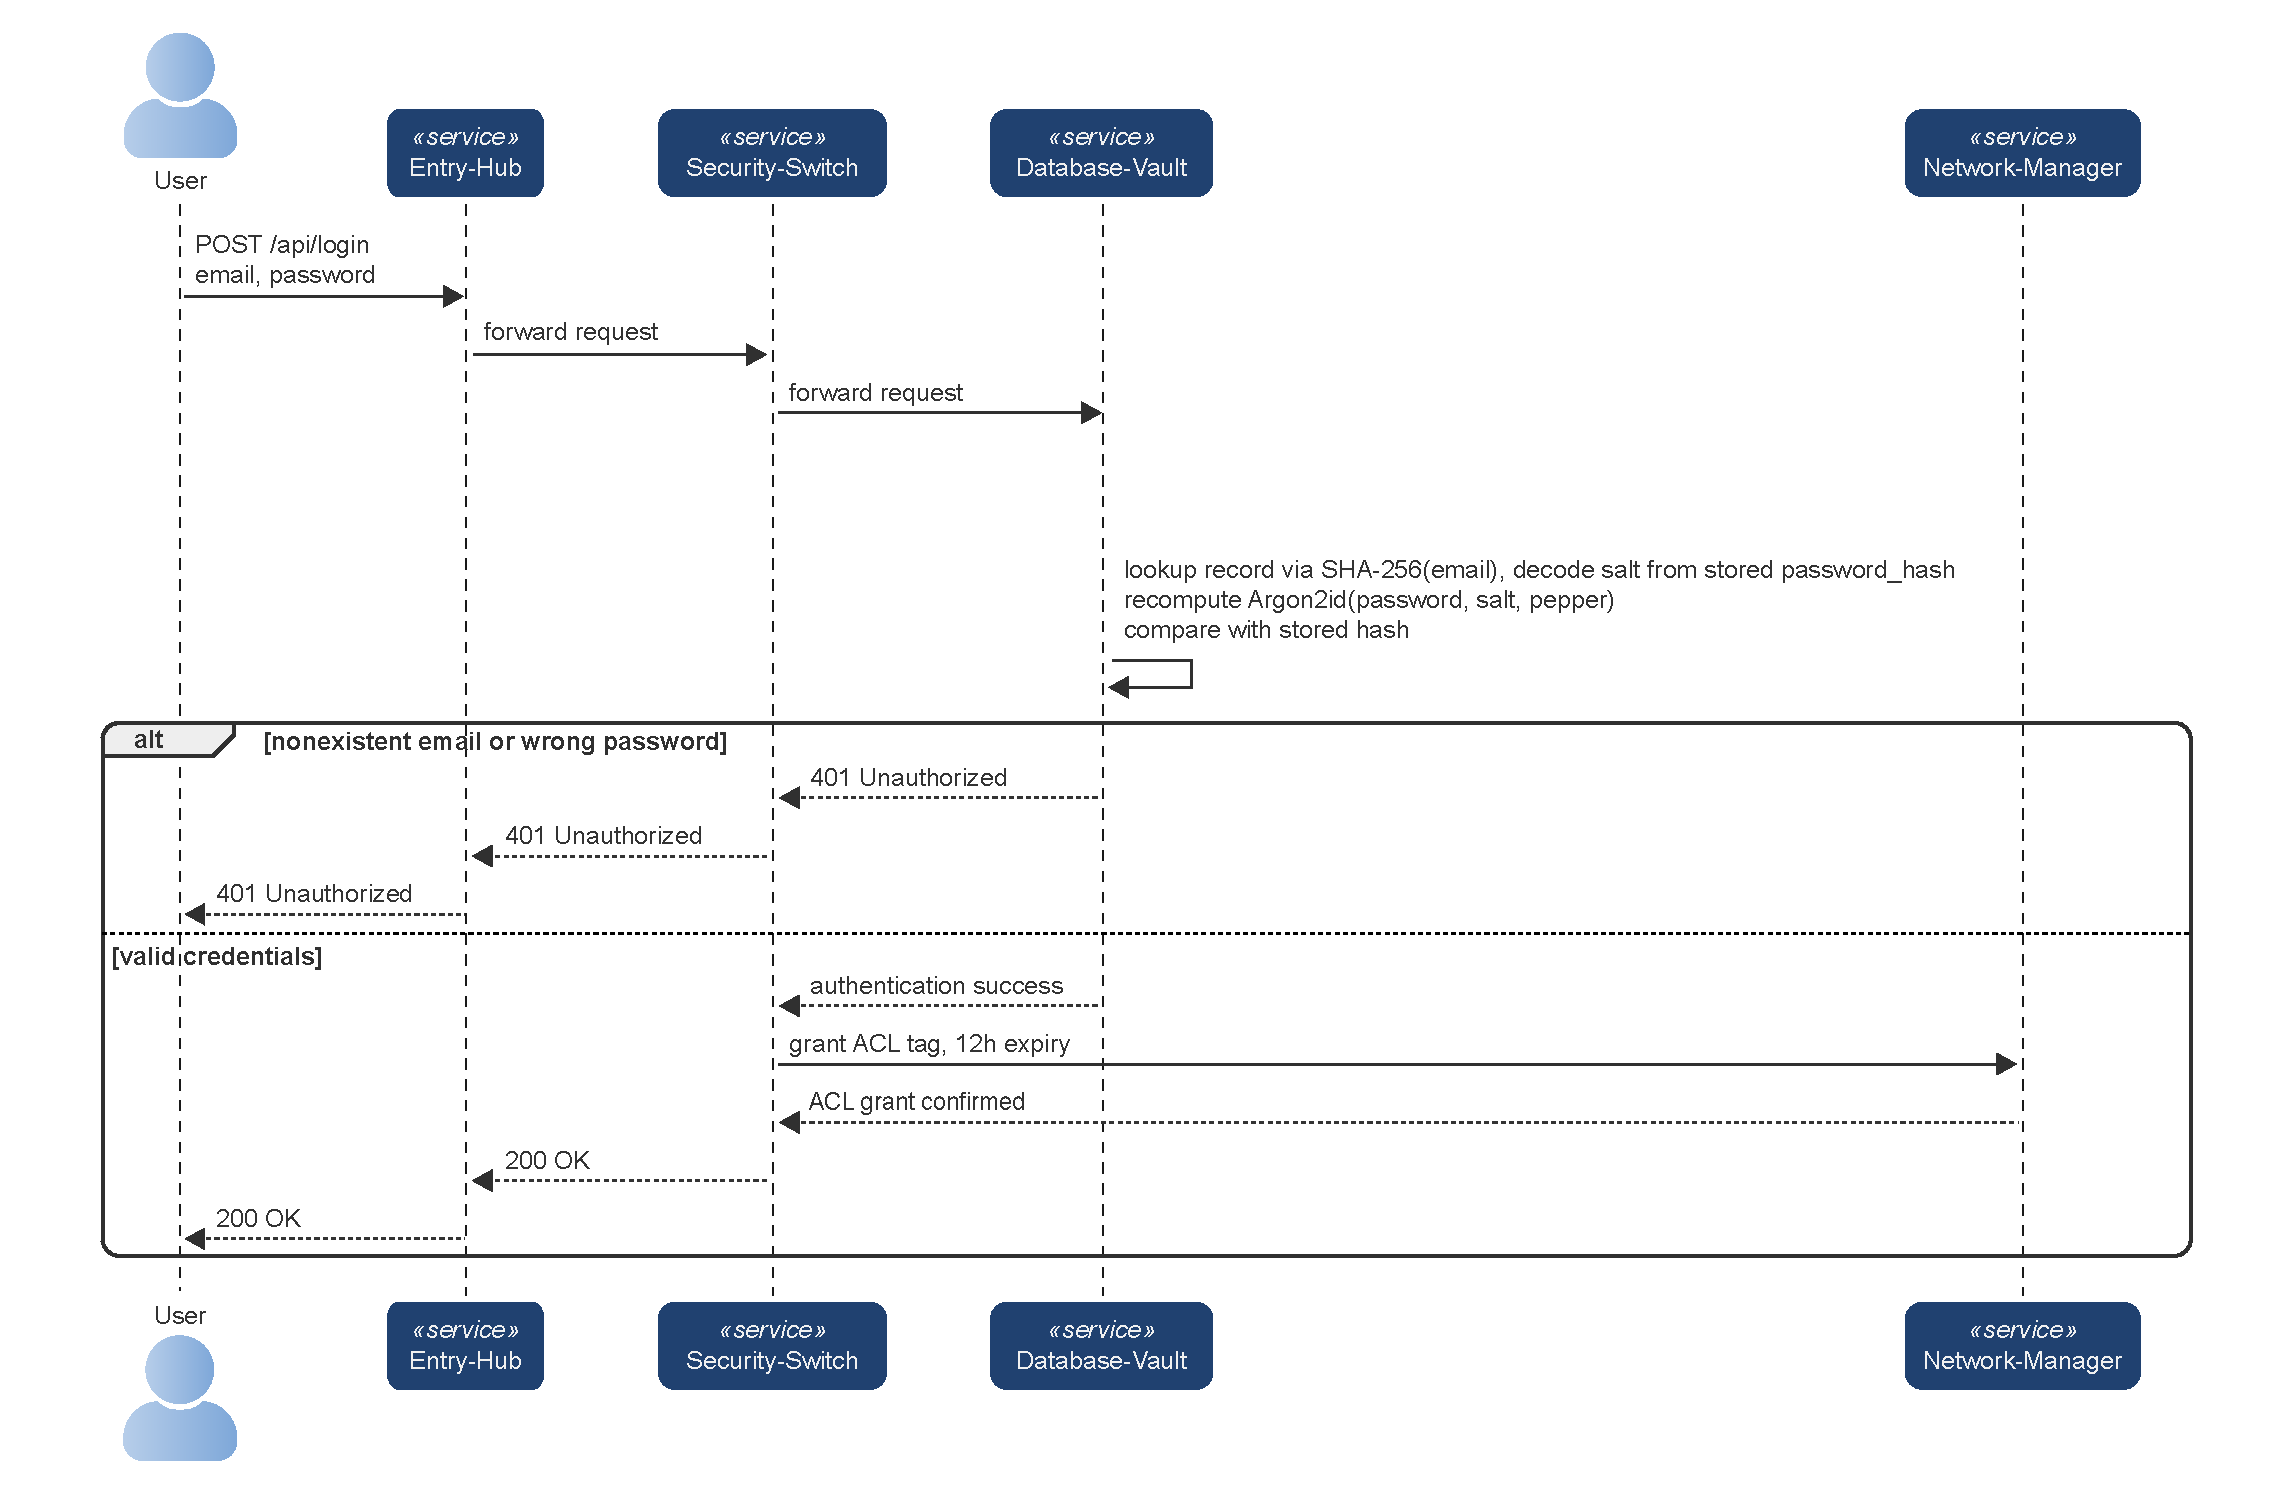
\includegraphics[width=\textwidth]{figures/04-usecases-sequence-uc02-login.pdf}
    \caption{Authentication sequence (UC-02).}
    \label{fig:uc02}
\end{figure}

\section{Post-authentication orchestration}

Authenticating a user, however, still does not give them access to anything. Access, in this system, is
a property of the network. Security-Switch asks Network-Manager to modify the network rules
at two different moments.

After a successful registration, it requests the creation of the user's identity on the mesh network and of
a pre-auth key, which travels back up the chain to the client inside the 201 response and which allows the user's
device to join the private network.

After a successful login, instead, it requests twelve-hour temporary access to Storage-Service.

Both steps, however, grant reachability, not read access: registration puts the
device in the network, login allows it to reach Storage-Service, but what opens the backups is
the SSH private key, which never leaves the user's device.
Knowing the user's credentials is therefore not a sufficient condition to access their backups.

How Network-Manager creates the mesh identity, applies the ACL tag and manages its expiry is the subject
of \autoref{chap:rete}.

\chapter{File storage and backup}
\label{chap:storage}

\section{SFTP-only access model}

Storage-Service stores the users' backups and is the only component the client talks to
directly after authentication.
Indeed, once authenticated, the user becomes able to reach it on the private network
and is therefore ready to manage their backups.

Before transmitting them, however, the user's client, through Restic \cite{restic-github}, deduplicates, compresses, and
encrypts the user's backups. Storage-Service therefore receives a sequence of encrypted blocks that it is not
able to decrypt.
When initializing the Restic repository, the client draws 32 bytes from \texttt{crypto/rand},
encodes them in base64 and uses them as the repository password \cite{ramusb-code-reposecret}.
From that password Restic derives the key that opens the file in which it keeps the actual encryption key,
generated at random when the repository is created \cite{restic-design}: it is the latter that protects the blocks.

This approach was designed to prevent the user from choosing a weak
password. The client saves the repository password on the user's device, with the same
permissions as the SSH private key. Its secrecy, like the responsibility of copying the keys to
a safe place, is left to the user. Should even a single one of the
credentials be lost, the user would have no way to access the content of their backups.

The fact that the users' data is encrypted, however, does not mean that it should be reachable by
anyone.
The only way to reach the blocks is in fact an authenticated SFTP session, inside the private
mesh network. On that session, the only possible operation is transferring files, and the only credential
accepted is the SSH key \cite{openssh-sshd-config}.

Left out are the other ways of authenticating and the other uses that SSH normally allows, such as executing a command,
opening a shell, or using the connection as a relay to reach other machines.

Moreover, only the accounts created by the service can log in, because the server accepts only
usernames of the form \texttt{user*} and root access is explicitly disabled.

OpenSSH's default list of cryptographic algorithms \cite{openssh-sshd-config} is deliberately broad
to guarantee compatibility with clients that do not support the modern and more robust algorithms, but here that
compatibility is not needed, and only risks weakening the system; therefore, the cryptographic
algorithms are also listed by hand \cite{ramusb-code-sshd-config}.

\section{Isolation and dynamic chroot}
\label{sec:isolamento}

Isolation between users rests on an operating system mechanism called chroot, which
confines a process inside a subdirectory: from that moment on that directory is, for the process, the
root of the filesystem, and outside of it there is no longer any path that the process can
name.

At registration, Storage-Service prepares for the new user the POSIX account that will inhabit that
space. The account has no traditional home directory and its shell is \texttt{/usr/sbin/nologin},
a program that merely refuses access.

For every POSIX user whose name matches \texttt{user*}, the rules
specified in \autoref{lst:sshd-match} are also applied.

\Needspace{10\baselineskip}
\begin{lstlisting}[language=sshdconfig, caption={The two per-user directives, from
\texttt{sshd\_config} \cite{ramusb-code-sshd-config}, with added comments.},
label={lst:sshd-match}]
Match User user*
    ChrootDirectory /storage/%u   # confines the session to the user's subtree
    ForceCommand internal-sftp    # enforces SFTP in place of the command requested by the client
\end{lstlisting}

Alongside the account, the directory structure illustrated in
\autoref{fig:filesystem-storage} is created. The root of the confinement belongs to root, while the
\texttt{data} subdirectory belongs to the user and is the only place where they can write.
Ownership by root is a requirement of the SSH server, which
refuses to confine a session in a directory writable by anyone else.

The result is that a connected user sees as the root of their filesystem the directory that
belongs to them, and the other users' directories are neither reachable nor listable in any way.

Normally an SSH server looks for the keys that authorize a connection in a file inside the user's
home, where the keys accepted for that account are listed. Here that file is not
consulted.
In its place, at every connection attempt, the server runs a dedicated binary, passing it the
username being presented. The binary runs under a system identity that has no other
duties on the machine and asks Database-Vault for that user's current public key over an
mTLS channel.

Whatever goes wrong produces the same outcome: the binary exits without printing anything
\cite{ramusb-code-authkeys-cmd}. The server receives an empty list of keys and denies the connection,
following the fail-secure principle \cite{owasp-fail-securely}.
There is no other place outside Database-Vault in which the SSH public keys are stored,
so a malfunction in Database-Vault prevents users from starting SFTP sessions.

\section{Backup and restore}
\label{sec:backup-restore}

The backup takes place entirely on the user's device. The client invokes Restic, indicating as the
repository the writable subdirectory inside the user's own confined space, reached via SFTP, and
requires it to authenticate with the private key generated at registration
\cite{ramusb-code-restic-sftp}, which has never left the machine and which no component of the
system has ever seen.

The path given for the repository is already relative to the root of the confinement.

The client resolves Storage-Service through MagicDNS on the mesh network,
and the resolution succeeds only as long as the temporary grant given by the last login is active:
once that has expired, the user's node no longer sees the service and the connection does not even start.
\autoref{chap:rete} describes how that grant is given and revoked.

\autoref{fig:uc03} summarizes the sequence, from the SFTP connection to the written data.

\begin{figure}[H]
    \centering
    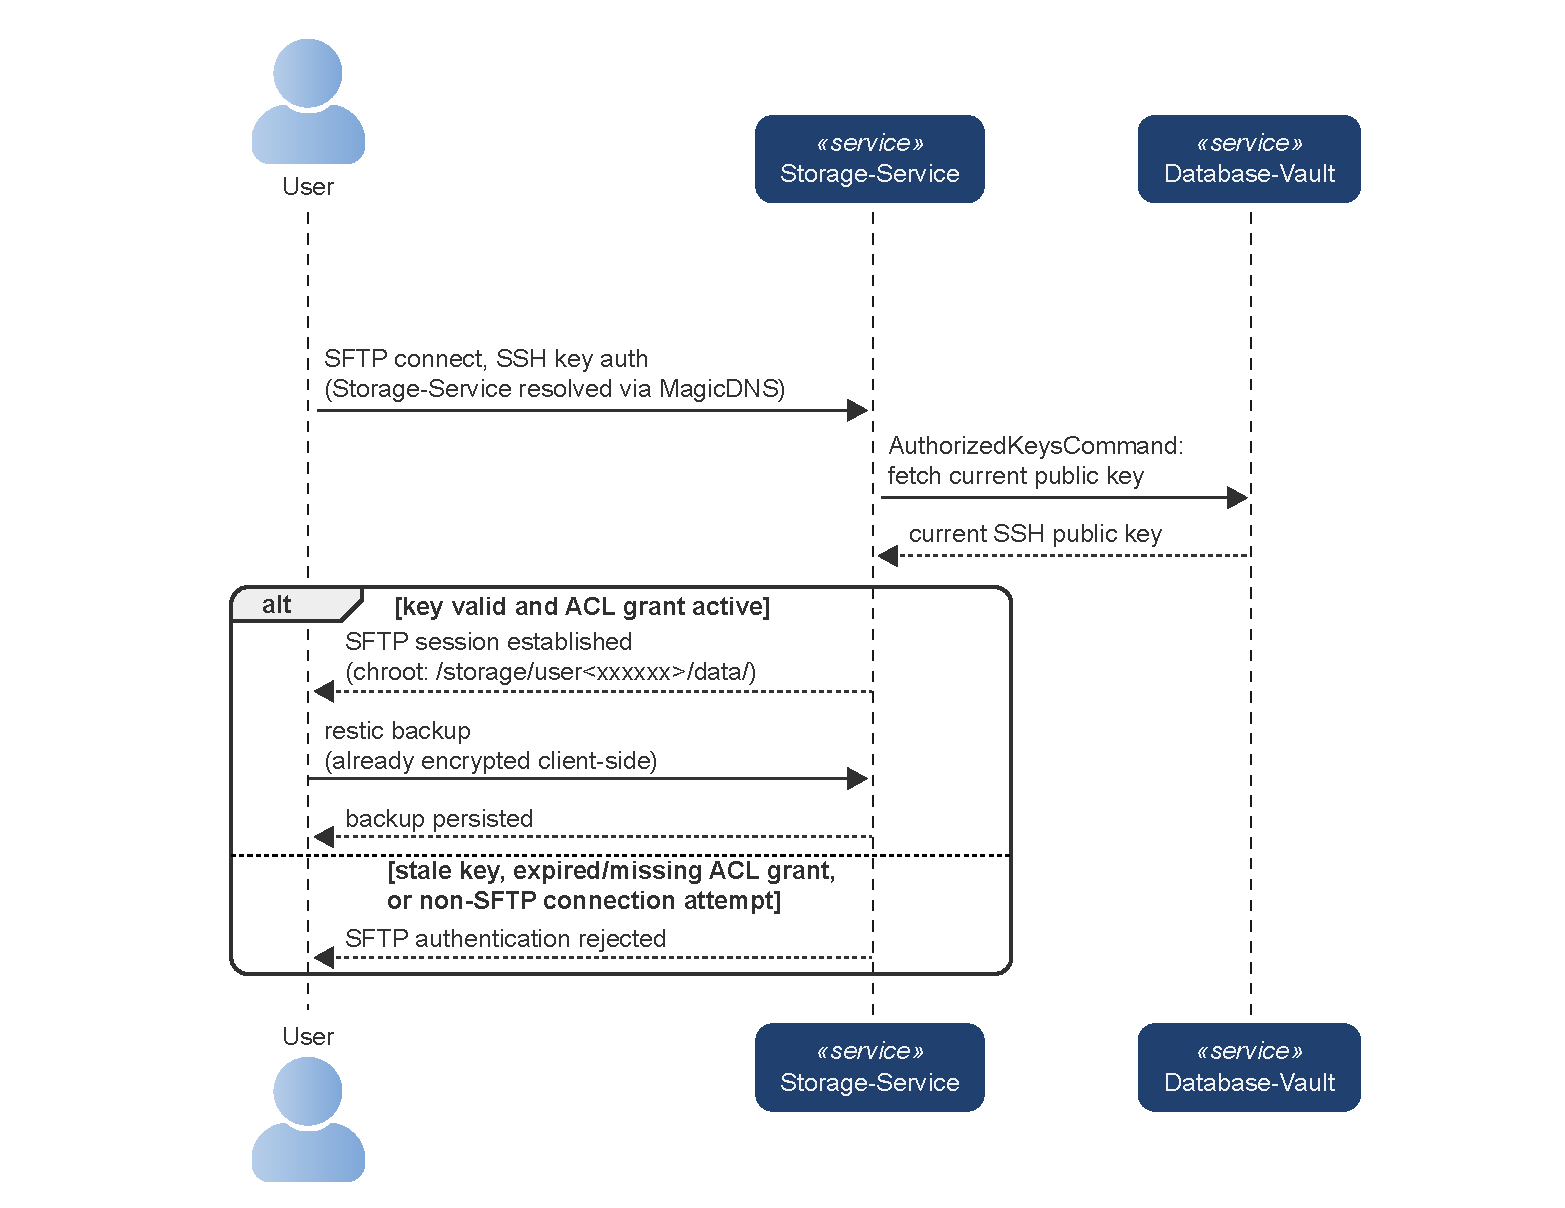
\includegraphics[width=0.8\textwidth]{figures/05-usecases-sequence-uc03-backup.pdf}
    \caption{Sequence for backing up a file (UC-03).}
    \label{fig:uc03}
\end{figure}

Restore follows the same path as backup; the only difference is the command issued to
Restic, which downloads the requested blocks and decrypts them on the user's device.

\chapter{Networking and mesh coordination}
\label{chap:rete}

\section{Network policies and reachability boundaries}

The trust zones of \autoref{fig:trust-zones} describe who can contact whom. The reachability boundaries
that derive from them are enforced by a network policy that Network-Manager publishes on Headscale.

Every node of the mesh network, be it a service or a user's device, carries one or more labels
called tags. The reachability rules are written on tags rather than on IP addresses, so as to
survive a change of a service's address, for example because it restarts on a different node.

Network-Manager collects all the rules into a single document and delivers it to Headscale only once,
at startup \cite{ramusb-code-acl-policy}.

Headscale in turn translates it into a packet filter: it tells every node that joins the network only about the
peers that the rules allow it to contact, and then sends it the subsequent updates concerning those peers.
In this way, a service that by policy must not contact another one is not even able to
see it in the network.

The rules, moreover, name only the party that opens the connection, so replies travel without a rule
in the opposite direction. In this way, for example, Security-Switch can contact Database-Vault, and the latter
can reply to the request, but is not able to initiate communication with it.

\section{Access grant lifecycle}

The two rules that concern the user are shown in \autoref{lst:acl-utente}. The tag
\texttt{TagStorageAccess} is temporary and is assigned at login; \texttt{TagMeshMember} is permanent and
is assigned when the device joins the network.

\Needspace{12\baselineskip}
\begin{lstlisting}[caption={The two rules that delimit the user's zones, from \texttt{policy.go}
\cite{ramusb-code-acl-policy}, with added comments.}, label={lst:acl-utente}]
{ // only an authenticated user, and Database-Vault, reach Storage-Service
    Action: "accept",
    Src:    []string{TagStorageAccess, TagDatabaseVault},
    Dst:    []string{dstAny(TagStorageService)},
},
{ // every registered user reaches Entry-Hub
    Action: "accept",
    Src:    []string{TagMeshMember},
    Dst:    []string{dstAny(TagEntryHub)},
},
\end{lstlisting}

At registration, Network-Manager creates for the new user an identity on Headscale and a pre-auth key,
that is, a single-use credential with which the device presents itself to the coordinator to join the network
\cite{ramusb-code-mesh-user}. The key is valid for fifteen minutes, and travels back up the chain of services to
the user inside the registration response.

The key is created already associated with the membership-only tag. The device that uses it therefore joins the
network and gains reachability to Entry-Hub's private network interface.

At login Network-Manager looks up the user's node and adds the second tag to it, then records an expiry
twelve hours from that moment \cite{ramusb-code-grant}.

Looking up the user's node, however, requires Network-Manager to keep a small SQLite database
containing the numeric identifier of the pre-auth key bound to the hash of the user's email, with the
schema shown in \autoref{lst:meshusers-schema}.

\Needspace{8\baselineskip}
\begin{lstlisting}[language=sql, caption={Schema of the email-to-pre-auth-key mapping table, from
\texttt{meshusers.go} \cite{ramusb-code-meshusers-schema}.}, label={lst:meshusers-schema}]
CREATE TABLE IF NOT EXISTS mesh_users (
	email_hash       TEXT PRIMARY KEY,
	pre_auth_key_id  INTEGER NOT NULL
);
\end{lstlisting}

The tag expiries are also persisted in the database, to prevent a restart of the service from turning
a twelve-hour grant into a perpetual grant. The schema of the table that holds them is shown in
\autoref{lst:grants-schema}.

\Needspace{10\baselineskip}
\begin{lstlisting}[language=sql, caption={Schema of the access grant table, from \texttt{store.go}
\cite{ramusb-code-grants-schema}.}, label={lst:grants-schema}]
CREATE TABLE IF NOT EXISTS grants (
	email_hash TEXT PRIMARY KEY,
	node_id    INTEGER NOT NULL,
	tag        TEXT NOT NULL,
	expires_at INTEGER NOT NULL
);
\end{lstlisting}

A periodic process, every five minutes, looks for expiries that have passed and revokes the expired grants
\cite{ramusb-code-sweep}. The row is deleted from the database before calling Headscale to remove
the tag, and the deletion is conditional on the exact expiry just read.
If in the meantime a login has renewed the grant, the expiry in the table no longer matches, so the deletion
touches no row and the sweep stops without contacting Headscale.
Calling Headscale first and deleting afterward would instead have risked also deleting the row
just rewritten by the concurrent login, taking away from the user a grant that had just been given.

\autoref{fig:acl-grant} summarizes the states that a user's node goes through.

\begin{figure}[H]
    \centering
    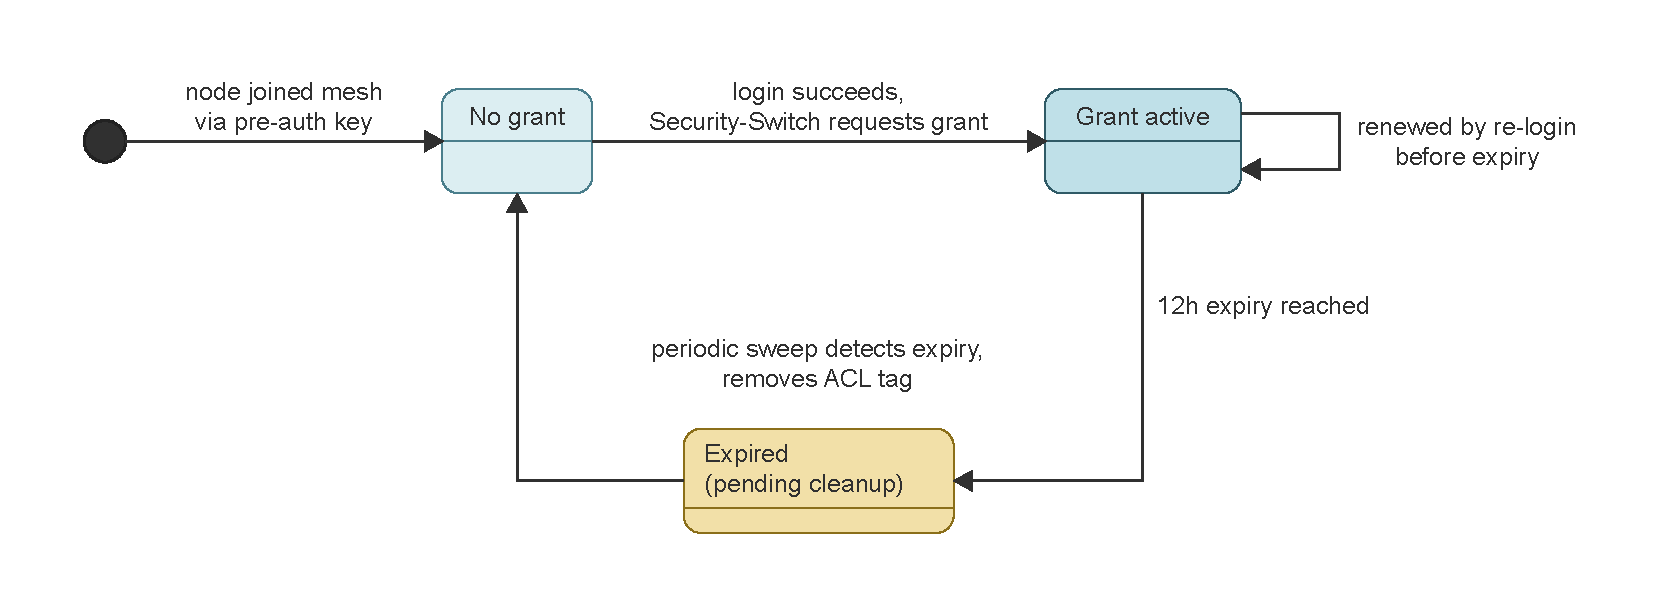
\includegraphics[width=\textwidth]{figures/10-operations-state-acl-grant.pdf}
    \caption{Lifecycle of the access grant associated with a user's node.}
    \label{fig:acl-grant}
\end{figure}

\section{The coordinator paradox: Headscale as a standalone service}
\label{sec:paradosso-coordinatore}

The Headscale documentation states that running Headscale on a machine that
belongs to the coordinated network is not recommended, because it can cause problems with name resolution through MagicDNS
\cite{headscale-faq}.

The coordinator must therefore remain outside the network it coordinates, and three consequences follow from this.

The first is that it cannot share a virtual machine or a container with any other component,
because all the others are members of the mesh.

The second is that the traffic with which Network-Manager creates the keys and assigns the tags cannot be
protected by its placement in the network, as is the case for every other internal call. It is the only
call between components of the system that crosses the public network, and the only one whose protection depends
entirely on mTLS and on the Headscale API key.

The third is that the coordinator must be publicly reachable, because a device that has not
yet joined the network must be able to contact it the first time in order to join the network.

Headscale, however, has a limitation that is relevant for RAM-USB: it offers no way to separate the coordination
protocol, which must be reachable by everyone, from the administrative API, which must be reachable only by
Network-Manager.
The separation was entrusted to a reverse proxy, which distinguishes the two surfaces based on the path
of the request \cite{ramusb-code-headscale-proxy}. Coordination requests pass without any check,
while administrative ones are accepted only if accompanied by a certificate issued by the
private Certificate-Authority, in addition to an API key that Headscale itself
requires. The administrative traffic is defended by two independent credentials because it is one of the most
sensitive surfaces.

The certificate presented by the proxy is instead issued by a public CA, for the same reason that
Entry-Hub's is.

\section{CG-NAT and the need for a dedicated public endpoint}

The central pool of not-yet-assigned IPv4 addresses was exhausted in 2011 \cite{icann-ipv4-2011}, and
to keep connecting new customers many Internet Service Providers have several subscribers share a single
public IPv4 address. The home router no longer receives a public address, but one
from the \texttt{100.64.0.0/10} block, valid only inside the operator's network and not
routable on the internet \cite{rfc6598}; it is a NAT managed by the operator that translates it into the shared
public address. This type of NAT is called Carrier-Grade NAT \cite{rfc6888}.
Since that NAT is not under the customer's control, the customer cannot open inbound ports on it
by themselves, and in general a server hosted at home is not reachable from the internet \cite{rfc6269}.
RAM-USB is designed so that it can also be hosted by home users, who therefore might not
have neither a public IPv4 address nor IPv6 connectivity. For this reason Headscale and Entry-Hub each reside on
their own Virtual Private Server, separate from the rest of the system. \autoref{chap:deployment} describes the actual placement of each component.

\chapter{Observability and metrics}
\label{chap:osservabilita}

\section{Publishing the metrics}

Operational metrics can typically reach whoever observes them in two ways: either someone else
periodically queries every service (\emph{pull}), or every service sends them on its own
initiative (\emph{push}).
RAM-USB adopts the second: every service publishes its own metrics once a minute,
on its own dedicated MQTT topic to the Mosquitto broker \cite{mosquitto-github}.
The choice stems from the fact that a \emph{pull} model would require Metrics-Collector to open a
connection to each of the six services, widening the mesh reachability rules discussed in
\autoref{chap:rete}.
Because the services publish on their own initiative, they are instead the ones that open the connection to the broker.
From there, Metrics-Collector reads the metrics and persists them in a database.

Operational metrics do not contain user data, but the system's metadata must be protected with the
same care; for this reason the communications take place inside the private network and are protected by mTLS,
with certificates issued by the internal CA.

Every publication carries as its body a six-field payload, shown in \autoref{lst:metrics-payload}.
The metrics in the payload refer to the minute in which they were sent.

\Needspace{10\baselineskip}
\begin{lstlisting}[caption={Structure of the metrics payload, from \texttt{payload.go}
\cite{ramusb-code-metrics-payload}.}, label={lst:metrics-payload}]
type Payload struct {
	Service               string  `json:"service"`
	Timestamp             string  `json:"timestamp"`
	RequestCount          int64   `json:"request_count"`
	ErrorCount            int64   `json:"error_count"`
	AverageResponseTimeMs float64 `json:"average_response_time_ms"` 
	ActiveConnections     int64   `json:"active_connections"`
}
\end{lstlisting}

The publications all use \emph{QoS 1} (at least once), in the MQTT classification \cite{oasis-mqtt-311}: the
broker guarantees that the message arrives at least once, at the cost of a possible duplicate. \emph{QoS 0}
(at most once) is ruled out because RAM-USB cannot afford to lose metrics silently; \emph{QoS 2}
(exactly once) is ruled out because the extra guarantee it offers (the absence of duplicates) is not needed here,
since a duplicate only results in two overlapping points at the same instant, invisible on the
chart.

\section{Reception and consistency check}

The published message must reach a single recipient. This property is enforced
by the Mosquitto ACL, which ensures that every service can only write to its own topic, while
Metrics-Collector can read from the \texttt{metrics/\#} topics without being able to write to them.

That ACL, however, does not prevent a compromised service, while staying within its own legitimate write
permission, from publishing a payload whose declared \texttt{service} field is a name different from
its own.
Metrics-Collector therefore revalidates every message independently, deriving the expected
service from the topic the message arrived on and comparing it with the one declared in the payload.
On any discrepancy it discards the message and records it in the logs.

\section{Time-series persistence}

Metrics-Collector persists the metrics in TimescaleDB \cite{timescaledb-github}, an extension of
PostgreSQL designed for a workload made almost entirely of time-ordered writes.

The \texttt{metrics} table has no primary key, since a row of metrics has no natural
identity. Moreover, TimescaleDB \cite{timescaledb-github} does not require one. It is organized in chunks by
time intervals on the \texttt{time} column: the two background policies in
\autoref{lst:metrics-policies} act chunk by chunk, based on their age. The first drops every chunk
older than thirty days; the second, after seven days, moves the chunks into a compressed columnar
format, grouped by service and ordered by descending time.

\Needspace{18\baselineskip}
\begin{lstlisting}[language=sql, caption={Automatic retention and compression policies of the
\texttt{metrics} table, from \texttt{000001\_create\_metrics\_table.up.sql} \cite{ramusb-code-metrics-schema}.},
label={lst:metrics-policies}]
SELECT create_hypertable('metrics', by_range('time'));

SELECT add_retention_policy('metrics', drop_after => INTERVAL '30 days');

ALTER TABLE metrics SET (
	timescaledb.enable_columnstore,
	timescaledb.segmentby = 'service',
	timescaledb.orderby = 'time DESC'
);
CALL add_columnstore_policy('metrics', after => INTERVAL '7 days');
\end{lstlisting}

\section{Metrics visualization}

An administrator checks the health of the system, without that consultation
ever touching the users' data since, by construction, the metrics do not contain any.
Grafana \cite{grafana-github} reads from TimescaleDB directly.

To contact TimescaleDB, in addition to reachability on the mesh network and Grafana's mTLS certificate,
a password is also required, following the same defense-in-depth principle already seen for Headscale's
administrative API in \autoref{chap:rete}.

The dashboard shows three panels, each a direct query on the \texttt{metrics} table: average
response time, throughput, and active connections.

\autoref{fig:metrics-flow} summarizes the entire pipeline just described, from publication on the MQTT
topic to the dashboard.

\begin{figure}[H]
    \centering
    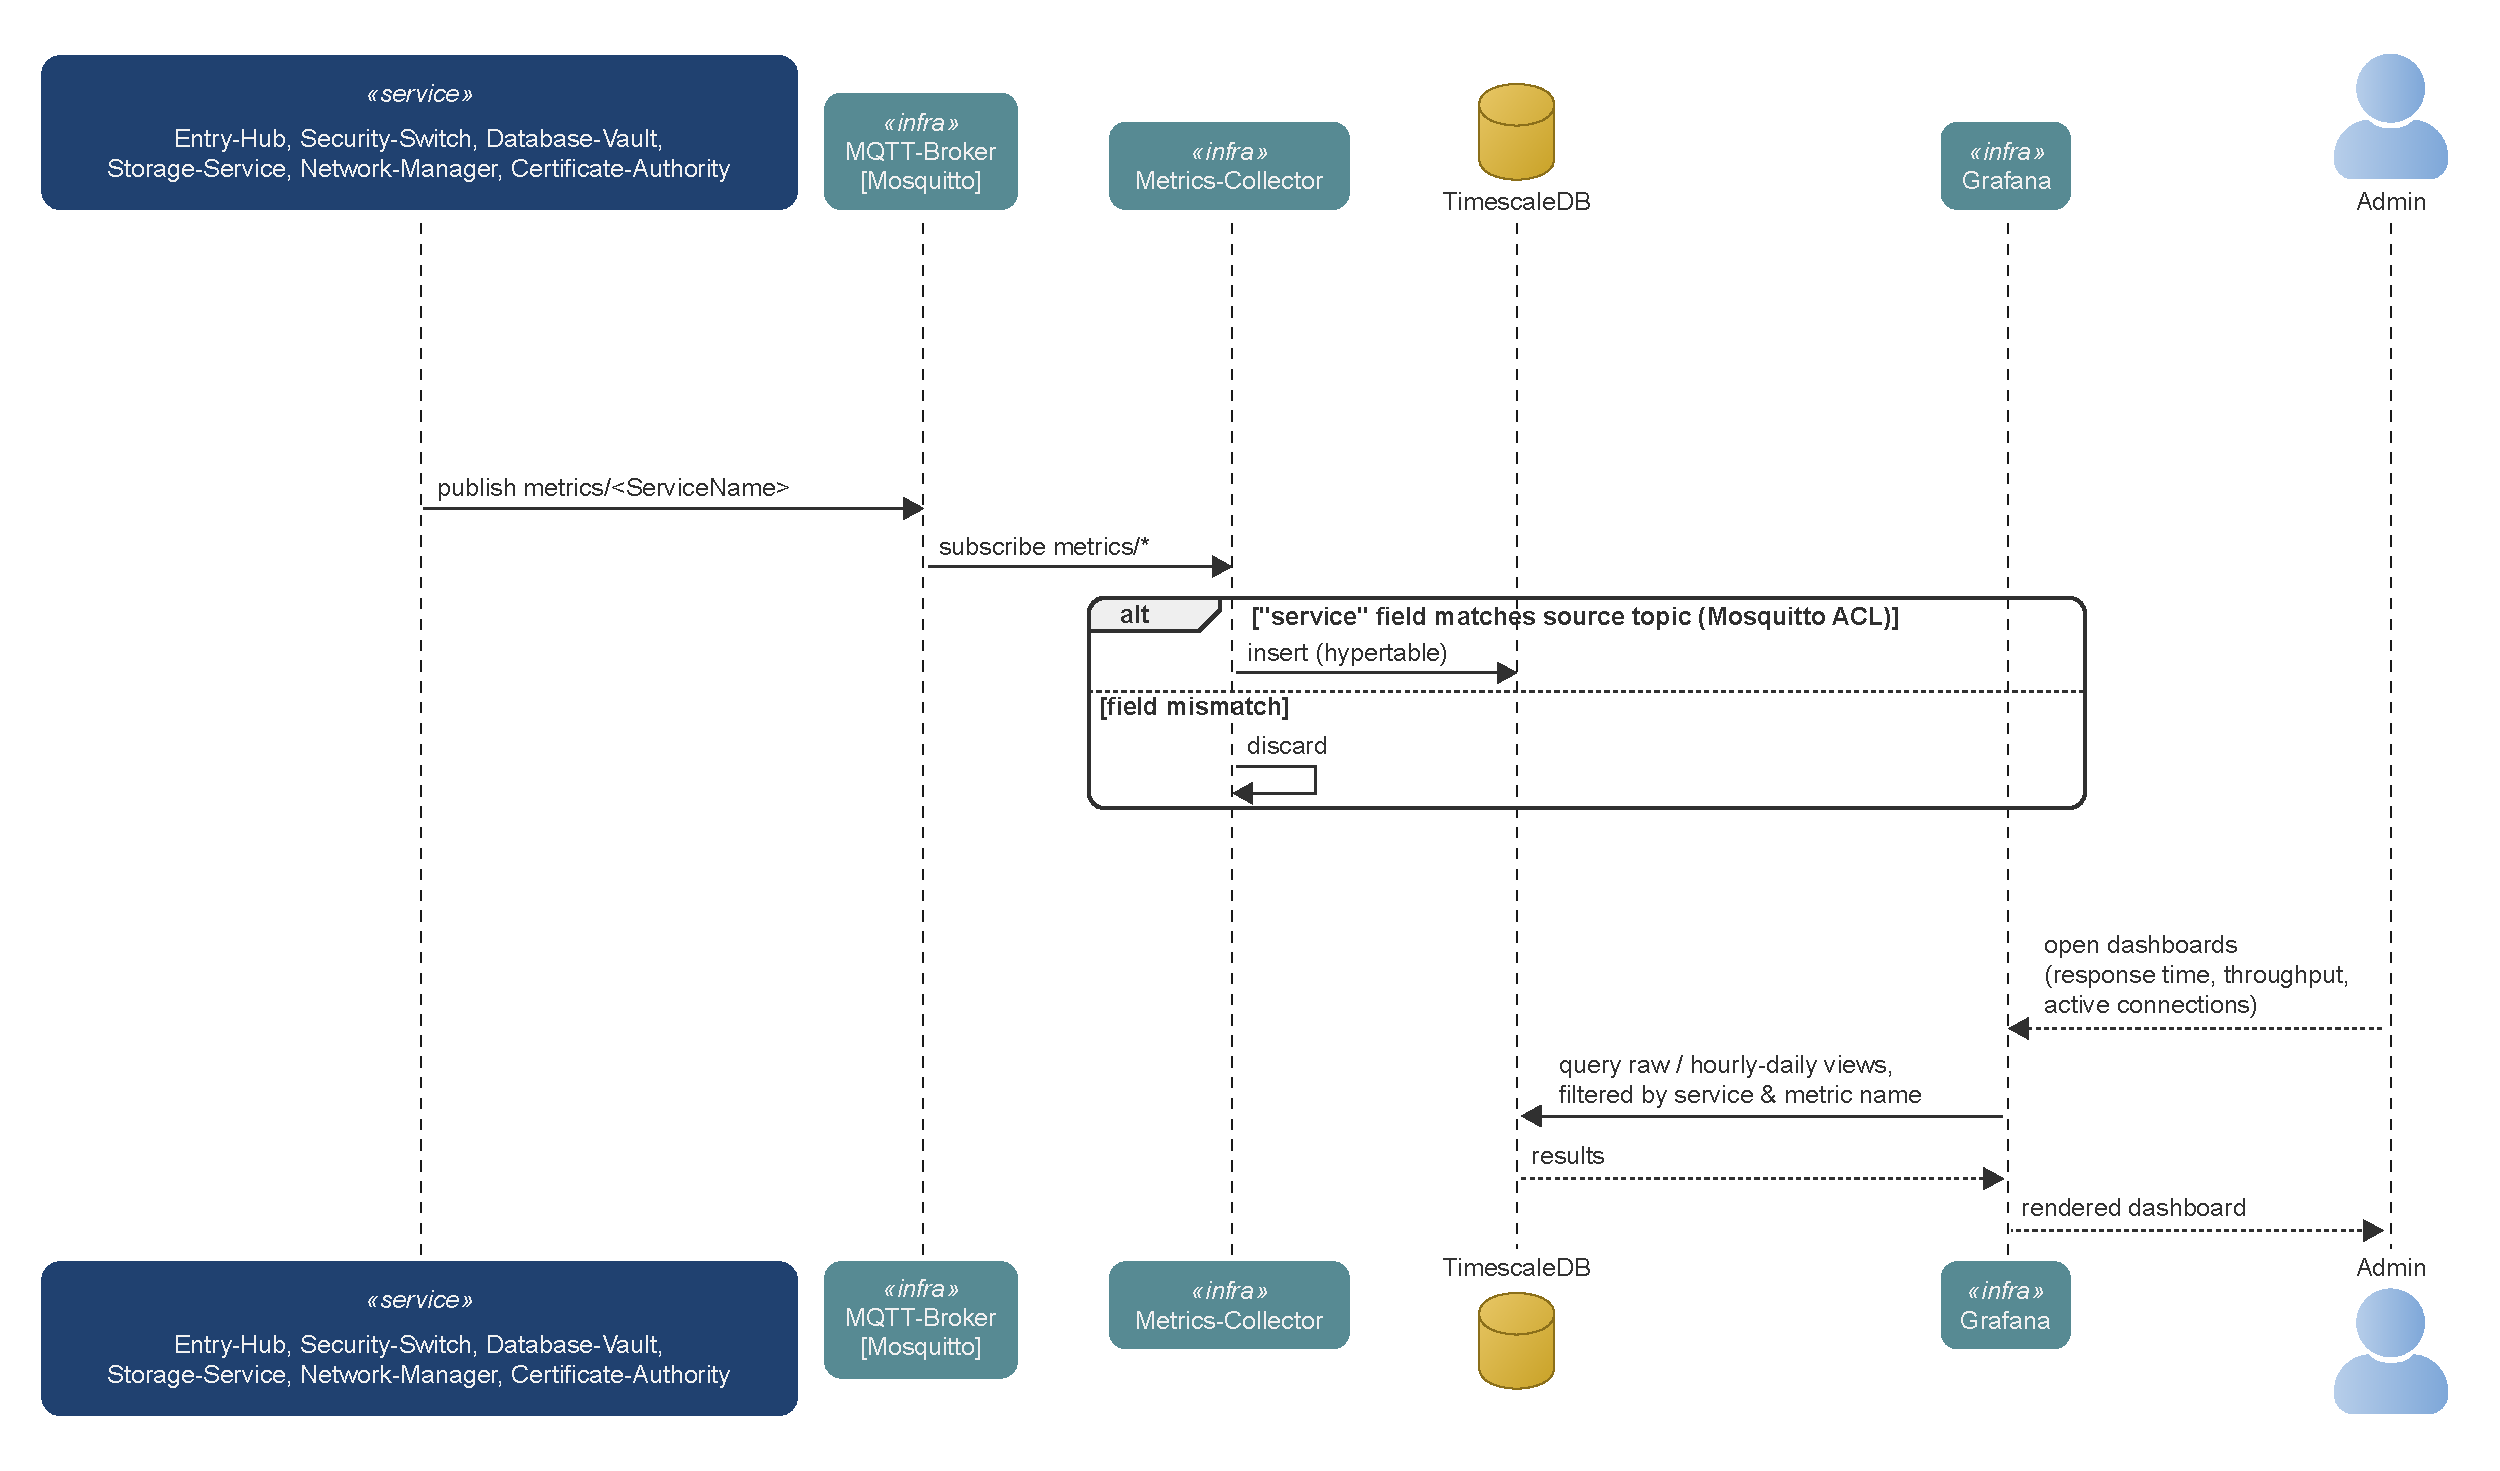
\includegraphics[width=\textwidth]{figures/11-operations-metrics-flow.pdf}
    \caption{Observability pipeline, from the publication of the metrics to the Grafana dashboard.}
    \label{fig:metrics-flow}
\end{figure}

\chapter{Testing and validation}
\label{chap:testing}

\section{The V-model and the four test levels}
For the testing of RAM-USB the V-model was adopted, an extension of the waterfall model in which
each specification phase is paired with a corresponding verification phase, written hand in hand with
the specification.

This approach was adopted because RAM-USB was deliberately treated as a
safety-critical system, in which a defect in production has serious consequences for the users of the system.
It was therefore essential that an error in the specification be detected well before implementation and
that testing be applied at several specification levels.

\autoref{tab:livelli-test} shows the correspondence between the requirement category and the test
level that verifies it, along with the technique used at that level.

\begin{table}[H]
\centering
\caption{Verification level associated with each specification level.}
\label{tab:livelli-test}
\begin{tabular}{@{}l p{\dimexpr0.55\linewidth\relax}@{}}
\hline
\textbf{Specification level} & \textbf{Verification level} \\
\hline
Component requirement & Unit testing with Go's \texttt{testing} package \\
Use case & Integration testing, bottom-up with drivers and stubs \\
Non-functional requirement & System testing, on the whole stack \\
User requirement & Acceptance checklist, walked through by hand on the corresponding use case \\
\hline
\end{tabular}
\end{table}

\section{Bottom-up integration strategy}

Integration starts from the innermost component and proceeds outward, in the order Database-Vault,
Storage-Service, Security-Switch, Network-Manager, Entry-Hub.

The choice to start from Database-Vault is dictated by the fact that it is at the same time the component
with the fewest outgoing dependencies and the one on which the largest number of functional requirements is concentrated.
Building it first, with drivers standing in for the components that invoke it and a stub standing in for
Storage-Service, the only component it invokes, ensures that the most sensitive component is also the one verified the longest.


\section{TDD: entry and exit criteria}

The entry criterion is that a test exists for every requirement, and that any failure of that test
occurs before the implementation of the requirement under test.

An example: requirement DV-F-15 requires that a nonexistent email and a wrong password produce the
same login outcome, indistinguishable from the outside.

The test that verifies it, \texttt{TestLogin\_NonexistentEmailAndWrongPassword\_AreIndistinguishable}
\cite{ramusb-code-login-test-dv-f-15}, calls \texttt{Login} with the two different credentials and requires
that the outcomes match exactly.

A test that has never been seen to fail, perhaps written after the code and passing on the first try, offers no
guarantee that it verifies anything: it might compare two values that are equal by construction, or not call the
function it is supposed to test at all.
For this reason, the test is written before the body of the \texttt{Login} function actually exists, and
it fails, providing proof that the test can recognize a wrong outcome.

Only after the test has failed does it make sense to write the complete body of \texttt{Login}, and only then does the
transition from failed test to passed test become useful information.

Writing tests first also helps to disambiguate and clarify requirements. Indeed, if a test cannot be written for a
requirement, the requirement is unclear or ambiguous and
consequently must be reworded more precisely.

There are three exit criteria, and they depend on the code under test. The first concerns only the validation
library, which requires more thorough tests because it is considered particularly sensitive.

\begin{itemize}
    \item in the validation library shared by Entry-Hub, Security-Switch, and Database-Vault
    (\autoref{sec:ciclo-richiesta}), every branch of every \texttt{if} or \texttt{switch} that decides whether to
    accept or reject a field must be traversed by at least one test case;
    \item no test that has already passed on the already integrated chain of components may fail;
    \item a change reruns not only the test written specifically for it but the entire test suite.
\end{itemize}

\section{Coverage and gaps in the test plan}

\texttt{go test -cover} measures, for each package of the codebase, the percentage of statements executed
at least once: \texttt{pkg/validation}, for example, reaches 98\%, because that is where the application logic lives,
while the \texttt{cmd} packages, which start each service, stay at 10--20\%, because verifying them is
the job of integration and system testing.

The exit criterion mentioned above for \texttt{pkg/validation} is a stricter measure that adds to
this one: it is not enough to execute almost all statements, every single branch of every \texttt{if} or
\texttt{switch} must have been taken by at least one test.

The test plan, however, is not free of limitations:
No test is planned for either protecting backups from tampering or rotating the
master key, currently out of scope, but essential in a project of this kind.
Load and stress testing, moreover, are planned but not yet designed. There are therefore no
reliable benchmarks of the system's behavior.
Every end-to-end test on the host involved a single user with a single small file in the backup, so neither
concurrency nor mutual isolation between two users has been put to the test.

\section{Automated pre-commit checks}

In addition to the entry and exit criteria, an automated verification chain runs before every
commit \cite{ramusb-contributing}. \texttt{golangci-lint} \cite{golangci-lint} is a runner that aggregates
multiple linters in a single pass; the RAM-USB configuration enables fifteen of them in total.

Among these, \texttt{gosec} \cite{gosec} looks for known security patterns in the code, and has been present since the
early stages of implementation.

A second extension introduced four linters targeting unreleased resources and mishandled errors:

\begin{itemize}
    \item \texttt{bodyclose} \cite{bodyclose} flags an HTTP response whose body is never
    closed, which therefore leads to a resource leak;
    \item \texttt{sqlclosecheck} \cite{sqlclosecheck} does the same for SQL rows and statements left
    open;
    \item \texttt{contextcheck} \cite{contextcheck} detects a function that does not propagate the
    \texttt{context.Context} received from the caller;
    \item \texttt{errorlint} \cite{errorlint} checks that errors are compared in the
    correct way.
\end{itemize}

These are complemented by Go's race-condition detector, invoked with \texttt{go test -race}.

The chain is completed by \texttt{govulncheck} \cite{govulncheck}, which compares the dependencies against a database
of known vulnerabilities but reports a problem only if the code actually reaches the vulnerable function,
and by two scanners designed to overlap with each other:
\texttt{gitleaks} \cite{gitleaks}, which looks for secrets already committed to the repository history, and
\texttt{trivy} \cite{trivy}, invoked in filesystem scan mode (\texttt{trivy fs .}), which
checks both dependencies and secrets independently of the two previous tools.

The redundancy of the last two is the application of the defense-in-depth concept to testing.

\section{Results: completed verifications}

The most significant campaign was run on real hardware, a Proxmox host with the components
deployed according to the placement described in \autoref{chap:deployment}.

The four use cases passed: registration and login succeeded, the backup completed and the
restore returned a file identical to the original.

\autoref{tab:verifiche} shows the properties checked on the running system.

\begin{table}[H]
\centering
\caption{Properties verified on the running system.}
\label{tab:verifiche}
\begin{tabular}{@{}p{\dimexpr0.34\linewidth\relax} p{\dimexpr0.56\linewidth\relax}@{}}
\hline
\textbf{Property} & \textbf{Observed result} \\
\hline
Hashing parameters & The string stored in the record shows \texttt{argon2id}, version 19,
memory 47104 KiB, two passes, parallelism one \\
Filesystem isolation & Confinement root owned by root with permissions 711,
user subdirectory 700 \\
Identity on the mesh & Every node is owned by the synthetic user
\texttt{tagged-devices}, never by the account created for the person \\
Grant duration & Expiry recorded at exactly twelve hours from the moment of login \\
Reachability boundaries & No node lists among its peers a component that the
policy forbids it from contacting \\
Restart survival & A service that is stopped and restarted comes back into service reusing
the identity on disk, without presenting the already consumed single-use token again \\
\hline
\end{tabular}
\end{table}

During the execution of the complete test plan, several defects emerged that had not been
caught by the earlier unit tests \cite{ramusb-known-issues}.

Two concerned the client and prevented backup entirely. The first was the SSH port: the client
connected to the default one, while the server listens on another. The second was the absence of
any host key policy: \texttt{ssh}, invoked by Restic without a terminal, had no
\texttt{known\_hosts} to check and no way to ask for confirmation, and refused the connection instead of
asking, so the first backup on every new machine always failed. A third concerned the configuration,
because the client has a single address for a service that exposes two on different listeners. A
fourth was a usage string documenting a syntax that the argument parsing cannot accept.

A fifth was more serious: the mTLS identity was not preserved from one startup to the next, so
no service survived the restart of its own container, because it retried the bootstrap with a
single-use token already spent.

Other small logic and implementation errors, too numerous to be reported in this thesis,
were detected and fixed thanks to the tests.

\chapter{Deployment}
\label{chap:deployment}

\section{Containerization and s6-overlay supervision}
\label{sec:s6-overlay}

Some RAM-USB services must run several independent processes in the same container and
therefore need a supervisor that starts them in the right order and restarts them when they go down.
The one used by RAM-USB is \texttt{s6-overlay} \cite{s6-overlay-github}.
Each supervised process is a directory under \texttt{s6-rc.d/}, declared as type \texttt{longrun};
its dependencies are files inside a \texttt{dependencies.d/} subdirectory, one for each process that
must be started: if, for example, process A must wait for process B to be ready,
\texttt{A/dependencies.d/} contains an empty file named \texttt{B}.
The startup order therefore arises from a graph declared between directories.
Storage-Service is the most complex case: the same Docker container is shared by four processes
\cite{ramusb-code-storage-s6-tree}: \texttt{tailscaled}, the actual mesh client; \texttt{sshd}, the
SFTP server (\autoref{chap:storage}); \texttt{identity-provisioner}, which keeps the X.509 certificate
for mTLS up to date; and the Go binary of Storage-Service itself, which exposes the internal HTTP API.
Each \texttt{longrun} process also has a \texttt{run} file and a \texttt{finish} file. The first is the
script that launches the actual binary \cite{ramusb-code-storage-s6-tree}.
If that process terminates, the supervisor relaunches it from scratch;
the second is optional and is used to delay the relaunch by a few seconds, so as to prevent an irreversible
startup error from turning into a continuous crash loop.

Not all services, however, need this complexity. Entry-Hub, for example, does not supervise
any secondary process: its membership in the mesh lives in a separate Docker sidecar,
\texttt{entry-hub-mesh}, which shares its network namespace. The following section explains how
this difference is tied to the choice of each service's base image.

\section{Why not all containers are distroless}
\label{sec:distroless}

A distroless image \cite{distroless-github} has neither a shell nor a package manager, which substantially reduces
the number of known critical vulnerabilities in containers \cite{wager2024distroless}.
A supervisor such as \texttt{s6-overlay}, however, needs a shell for its own startup scripts.
Any service that must run more than a single Go binary therefore cannot be distroless.
Consequently, the only distroless service is Entry-Hub \cite{ramusb-code-dockerfile-entry-hub}, while
the other six use \texttt{debian:bookworm-slim} or \texttt{alpine}, as shown in
\autoref{tab:immagini-base}.

\begin{table}[H]
\centering
\caption{Base image of each service and the processes sharing its container.}
\label{tab:immagini-base}
\begin{tabular}{@{}l p{\dimexpr0.3\linewidth\relax} p{\dimexpr0.38\linewidth\relax}@{}}
\hline
\textbf{Service} & \textbf{Base image} & \textbf{Shares the container with} \\
\hline
Entry-Hub & distroless & none (mesh in a separate sidecar) \\
Security-Switch & debian:bookworm-slim & \texttt{tailscaled} \\
Network-Manager & debian:bookworm-slim & \texttt{tailscaled} \\
Storage-Service & debian:bookworm-slim & \texttt{tailscaled}, \texttt{identity-provisioner}, \texttt{sshd} \\
Database-Vault & \texttt{postgres:17} (Debian) & \texttt{tailscaled}, \texttt{postgres} \\
Metrics-Collector & \texttt{timescaledb} (Alpine) & \texttt{tailscaled}, \texttt{timescaledb} \\
Certificate-Authority & \texttt{step-ca} (Alpine) & \texttt{step-ca} (mesh in a separate sidecar) \\
\hline
\end{tabular}
\end{table}

Extending distroless to more services or choosing distributions other than those listed in
\autoref{tab:immagini-base} is an issue that has not yet been addressed.

\section{Local Docker vs Proxmox VE: two levels of isolation}
\label{sec:docker-vs-proxmox}

It would be natural to think of Docker and Proxmox VE \cite{proxmox-ve} as two alternatives for the same
isolation need. In reality they operate at two different levels. Docker is a containerization engine:
it isolates a process at the operating system level, sharing the kernel with the host, so that each container
sees its own filesystem, its own network, and its own process tree without the cost of a second
kernel \cite{docker-overview}. It thus guarantees portability across operating systems and per-service
isolation, identical in development and in production.

Proxmox instead adds, on top of each Docker container, the isolation boundary of a KVM virtual machine,
with its own kernel, or, alternatively, that of an LXC system container, lighter but sharing the kernel
with the host. Each service therefore runs inside its own Docker container, but that
Docker container in turn runs inside its KVM virtual machine or inside its LXC container.
Choosing Proxmox also brings another advantage: it paves the way for live migration of the KVMs
and, with more nodes, for high availability.

Storage-Service, Database-Vault, and Network-Manager are assigned to KVM guests, while the remaining
services are assigned to unprivileged LXC containers, in which the container's root user is therefore mapped
to a non-root user of the host.
Entry-Hub and Headscale stay outside Proxmox entirely, each on its own dedicated public VPS, for the
reasons explained in \autoref{chap:rete}.

The choice between KVM and LXC depends, for almost all services, on the level of isolation they require.
LXC containers share the kernel with the host system, so they are not fully isolated, but
they need very few resources, so the host can run several of them at the same time. For this
reason they are the default choice.
The services that hold user data, manage network policies, and store backups need
greater isolation, because their compromise could cause irreparable damage.
Storage-Service also needs to run \texttt{setuid} and \texttt{chroot} to isolate POSIX
users (\autoref{sec:isolamento}): doing so inside an LXC container, itself already a namespace,
would add a second level of UID mapping. A KVM avoids stacking
two isolation mechanisms that do not compose cleanly \cite{ramusb-proxmox-storage-service}.

\section{Distributed topology}
\label{sec:topologia-distribuita}

The repository contains eleven separate Compose files under \texttt{deployments/compose/}
\cite{ramusb-code-compose-tree}. Ten correspond to the internal components
(\autoref{chap:architettura}); the eleventh, \texttt{tailscale-test.yml}, supports testing.
Containerization of the client is instead left to future work.
Each component's file remains independent of the others because every service is designed to be
started, stopped, or moved to a different Proxmox node, into a different KVM guest or LXC container.

\autoref{fig:architecture-deployment} summarizes the production topology.

\begin{figure}[H]
\centering
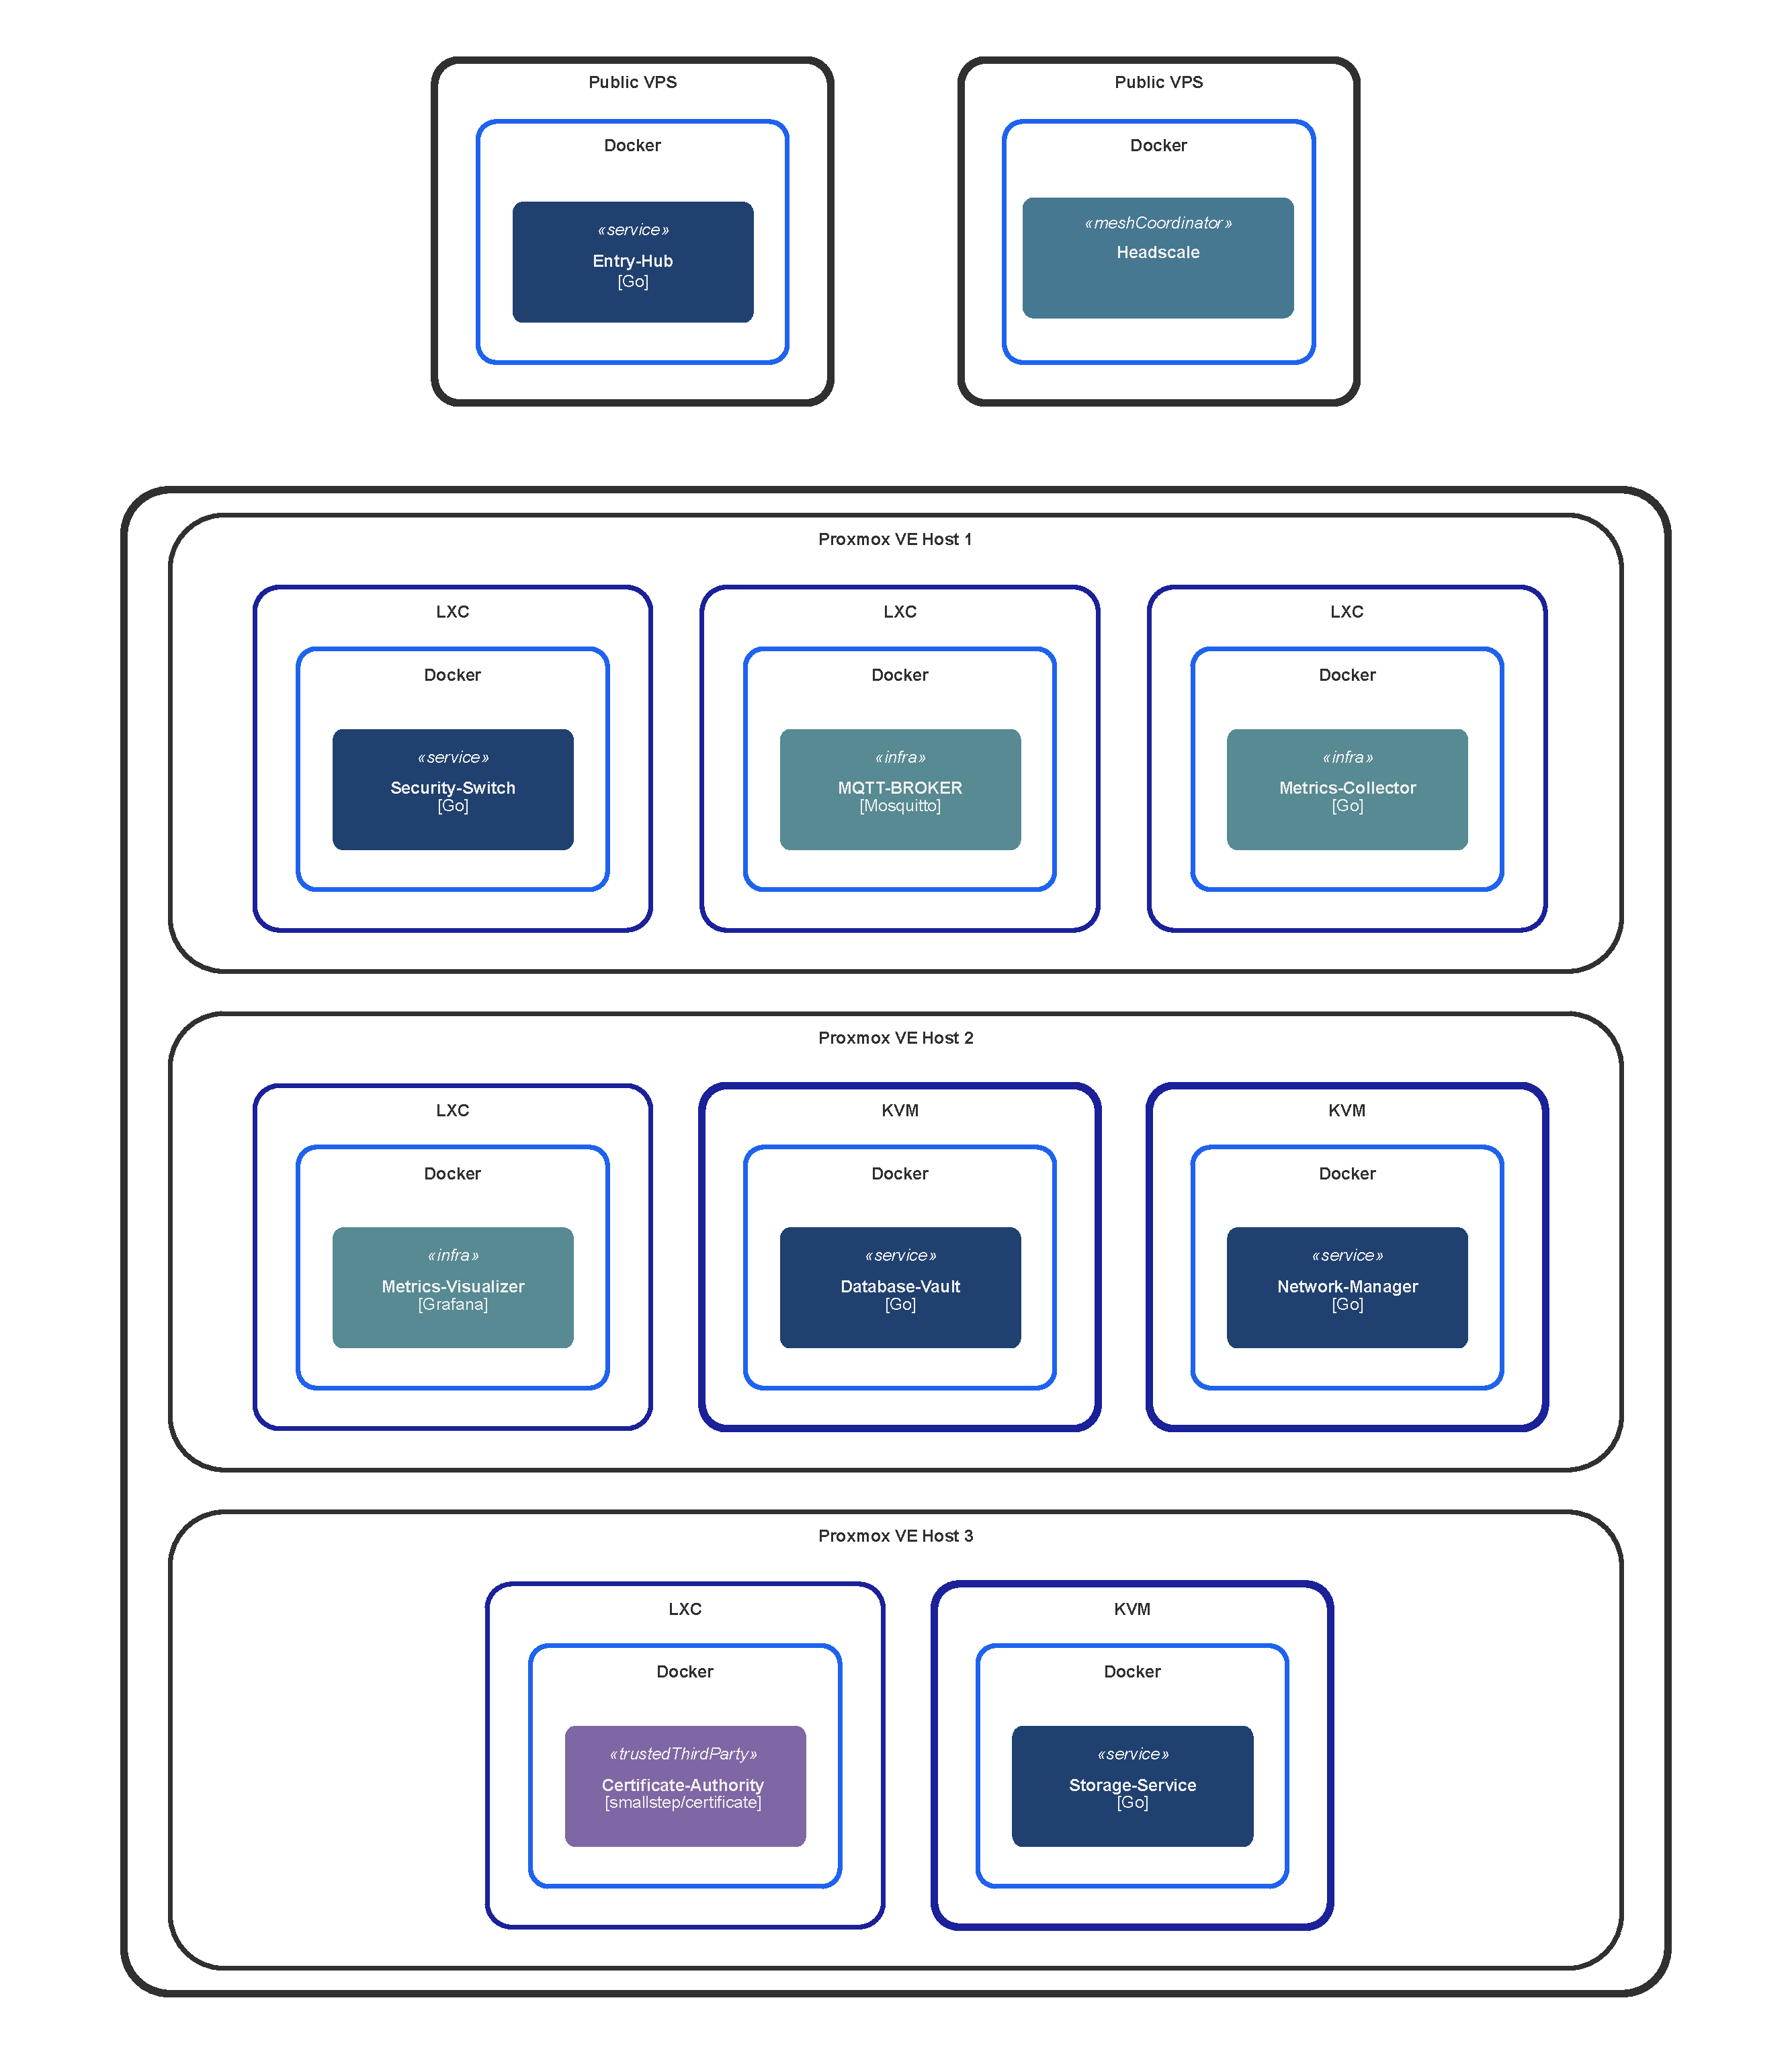
\includegraphics[width=0.95\textwidth]{figures/02-architecture-deployment.pdf}
\caption{Target production topology.}
\label{fig:architecture-deployment}
\end{figure}

\section{High availability and resilience: current state and limitations}
\label{sec:ha-limiti}

The service remains available to users only as long as the components that take part
in a request's path remain available.

The number of available physical nodes determines how much resilience and fault tolerance RAM-USB
can achieve: each added node unlocks one more property.

With a single physical node, \texttt{s6-overlay} supervision restarts a crashed process inside
a Docker container (\autoref{sec:s6-overlay}), but does not cover the unavailability of the physical node the
service runs on. Moreover, the most that can be achieved is local disk redundancy, for example with
RAID-10.

A second node unlocks zero-downtime migration of KVMs from one node to another, to balance the
load or free one up for maintenance \cite{proxmox-qm-migration}.
LXC containers, on the other hand, cannot be live-migrated, only restarted elsewhere \cite{proxmox-pct-migration}.

With at least three nodes and storage replicated with Ceph, the system becomes a hyperconverged cluster,
able to offer automatic recovery after the failure of a physical node, in addition to the planned
relocation of a healthy one.

The nodes, however, must be on the same low-latency network in order to cooperate, since the Proxmox cluster
stack requires a latency below 5 ms between all nodes \cite{proxmox-cluster-manager} to operate
stably.

Even with the best fiber available, two nodes far apart cannot reach such a low
latency. Extending the Proxmox backend to multiple sites would require a different mechanism, not yet planned.
At present, hyperconvergence and geo-distribution are mutually exclusive.
Achieving both at the same time remains an open problem outside the scope of RAM-USB.

\chapter{Critical analysis of security properties}
\label{chap:sicurezza}

\section{Attack scenarios and mitigations}
\label{sec:scenari-attacco}

The previous chapters describe RAM-USB's defenses from the point of view of those who build them.
This section rereads them from the point of view of those who try to compromise them.

\subsection{Email address enumeration at registration}

\texttt{POST /api/users} is a public endpoint that responds 201 if the submitted email is available
and 409 if it is already registered, without specifying whether the conflict comes from the email or from the
SSH key. However, anyone who submits a client-validated password and a freshly generated SSH key,
and therefore one that is certainly unique, has already ruled out that the conflict is on the SSH key.

\autoref{sch:enumerazione} summarizes the procedure, with the following symbols:

\begin{itemize}
    \item $e$: the candidate email address;
    \item $p$: a client-validated password;
    \item $k$: an SSH public key generated by the attacker;
    \item $r$: the HTTP status code returned by \texttt{POST /api/users}.
\end{itemize}

\begin{schema}
\centering
$\begin{array}{rl}
1. & k \leftarrow \mathrm{KeyGen}() \\[4pt]
2. & r \leftarrow \mathrm{POST}\ \texttt{/api/users}(e, \, p, \, k) \\[4pt]
3. & r = 409 \;\Longrightarrow\; e \mbox{ already registered}
\end{array}$
\caption{Checking whether an email address is already registered.}
\label{sch:enumerazione}
\end{schema}

Login, on the other hand, hides this information much better, returning the same 401 both for a nonexistent
email and for a wrong password, with the same log and the same response time
(\autoref{sec:login}). That protection was never extended to registration.

The registration endpoint also has a side effect far more serious than enumeration, caused
by the fact that the system does not verify that whoever submitted the registration credentials actually
owns them.

A malicious actor who registers with an email that does not belong to them permanently prevents registration
by its legitimate owner, forcing the owner to use a different email address.

Both problems could be solved by responding to registration requests identically in
all cases, for example always with a 202, while the actual outcome would travel out-of-band, in a
confirmation email sent to the given address.

This, however, requires rethinking how to deliver to the user the pre-auth key that currently travels inside the
201 registration response.

\subsection{Administrative access to credentials}
\label{sec:accesso-credenziali}

Email and password pass, encrypted in transit, through Entry-Hub, Security-Switch, and Database-Vault.
Whoever controls even just one of these processes can read them at the point where they are in plaintext in memory.

At rest, however, the password is never recoverable, not even by an administrator with full
access to the database. The email, instead, is recoverable by an administrator who holds the master key.

The problem of credentials captured in transit could be mitigated by encrypting the credentials end-to-end
between the client and Database-Vault, but in this case the problem would still not be completely
solved, and additional complexity would be introduced into the system. The only real solution is to use a zero-knowledge
authentication system.

\subsection{Offline address verification from a database copy}

An attacker who holds a stolen copy of the database can immediately check
whether a suspected email address is present in the database or not. The attacker only needs to compute the SHA-256 hash
of the candidate address and compare it with the hashes stored in the database.

Extracting an arbitrary email from the database, however, requires a very different effort.
The attacker cannot decrypt the email without the master key and is therefore forced to attack its SHA-256
hash.
The attacker could, however, identify some emails if they appeared in public dictionaries, using a
dictionary attack; otherwise, the only viable path remains a brute-force attack.

\autoref{sch:bruteforce} formalizes the procedure, with the following symbols:

\begin{itemize}
    \item $D$: the set of digests present in the stolen database;
    \item $W$: a dictionary of plausible addresses;
    \item $e$: an email address drawn from $W$.
\end{itemize}

\begin{schema}
\centering
$\begin{array}{rl}
1. & \forall e \in W: \\[4pt]
2. & k_h \leftarrow \mathrm{SHA\mbox{-}256}(\mathrm{lower}(e)) \\[4pt]
3. & k_h \in D \;\Longrightarrow\; e \mbox{ already registered}
\end{array}$
\caption{Search for registered addresses from the stolen database, by dictionary or brute force.}
\label{sch:bruteforce}
\end{schema}

Both of these vulnerabilities can be mitigated by replacing the plain digest with an HMAC-SHA256 keyed with
a dedicated pepper, generated with sufficient entropy and distinct from the one used for password hashing.
An attacker who steals the database does not automatically obtain the pepper as well, and therefore cannot
recover the email addresses in a reasonable time.

The theft of user credentials, although very serious, does not compromise the backups and does not prevent
the user from accessing them. Accessing them requires the SSH private key, which the user keeps locally.
Nor are the stolen credentials enough to delete or modify the user's account, because the system does not
guarantee users the right to be forgotten.

\section{Failure isolation}

This section analyzes which of the User Requirements remain guaranteed even in the worst case: the
full compromise of a service.
It also analyzes how to resolve the compromise where possible, provided that it is detected.

\begin{table}[H]
\centering
\caption{User Requirements verified in this section against the full compromise of a service.}
\label{tab:ru-isolamento-fallimenti}
\begin{tabular}{@{}l p{\dimexpr0.75\linewidth\relax}@{}}
\hline
\textbf{Requirement} & \textbf{Description} \\
\hline
RU-04 & Be able to access one's own backup only after having authenticated. \\
RU-05 & Have the guarantee that no one, administrators included, can read one's own backups. \\
RU-06 & Have the guarantee that no one, administrators included, can read one's own
access credentials. \\
RU-08 & Have the certainty that one's own data is isolated from that of other users. \\
\hline
\end{tabular}
\end{table}

The remaining properties fall outside this verification: RU-01, RU-02, RU-03, RU-07, and RU-10 are functional
or availability requirements that a compromised service easily denies, and therefore do not require
a case-by-case verification; RU-09 remains out of scope as stated in \autoref{chap:requisiti}.

\subsection{Entry-Hub}

An attacker who gains control of Entry-Hub can read, block, or tamper with every registration and login
request. They can also abuse its reachability toward Security-Switch,
Certificate-Authority, and the MQTT broker.

Tampering, however, does not affect RU-05, because the Restic repository password originates on the user's
device and never passes through Entry-Hub, before, during, or after tampering (\autoref{chap:storage}).
Nor does it affect RU-04, because an already authenticated user reaches Storage-Service directly over the
mesh, without ever going through Entry-Hub (\autoref{chap:architettura}).
The attacker can, however, block or alter new registration and login requests.

The compromise, if detected, can easily be contained. Network-Manager can revoke
a node's membership in the mesh, cutting the compromised Entry-Hub instance off from the network, and while
the cause of the compromise is being investigated, a new Entry-Hub instance can be started in a KVM on
Proxmox, ideally on a different node (\autoref{sec:docker-vs-proxmox}). In this way, registration of new users remains impossible, since the KVM might
not have a reachable public address, but user login can take place without problems,
since it happens on the handler reachable only from the private mesh network.


\subsection{Certificate-Authority}

An attacker who gains control of Certificate-Authority could sign a valid mTLS certificate
for any \texttt{organization} (\autoref{sec:pki}) and thus impersonate any internal
service, or refuse to issue updated certificates to services that request a renewal.

Realistically, however, they cannot contact anyone other than the MQTT broker, because according to Headscale's ACL rules, the CA can only
respond to calls from internal services, without being able to initiate new communications (\autoref{sec:trust-zones}).

This does not affect RU-05 or RU-06, since the CA plays no role in backup encryption
(\autoref{sec:backup-restore}) nor in the derivation of the credential keys
(\autoref{chap:autenticazione}).
RU-08 also remains guaranteed, as it has no connection with the CA.
What breaks down is mutual authentication between services.
The services, however, being unable to renew their certificates, can no longer communicate, so
once the certificates expire, the entire system comes to a halt.

The failure of authentication between services can easily be detected.
When this happens, until the investigation into the compromise is concluded, a new instance of the
CA can be restarted in a KVM on Proxmox, ideally on
a different node, ensuring greater isolation than that offered by an LXC (\autoref{sec:docker-vs-proxmox}).


\subsection{Database-Vault}

An attacker who gains full control of Database-Vault obtains the pepper and the master key, and with
the latter decrypts every email stored in the database.
However, they do not obtain the password with the same ease. For that, the attacker has two possible paths:
the first is to steal the database and attack it offline, at the cost of Argon2id's computation time (\autoref{tab:phc}).
This approach normally requires a great deal of time and considerable computational resources, making it
practically infeasible.
Without the pepper to protect them, however, weak and very common passwords can easily be cracked with
a dictionary attack, even if protected by a slow and expensive hashing algorithm such as Argon2id.

The second path is far more insidious: the attacker can remain passive and observe the calls to Database-Vault.
In this way, not only can they read the credentials of new users, but, by analyzing login requests and
following them all the way to the database, they can identify which hashes the passwords sent by users correspond to.
This requires the malicious actor to remain hidden for the time needed to receive login
requests from all the users who registered before the infiltration.

RU-06 therefore no longer holds at all for the email, and is reduced to a time cost for complex and uncommon
passwords.

RU-05 nonetheless remains guaranteed: Database-Vault has no access to Storage-Service's filesystem; it only has the
ability to ask it to create an account (\autoref{chap:architettura}). RU-08 also remains guaranteed, for
the same reason.

In this case, even if the active attack were detected, there would be nothing left to do; one must assume
that the database has already been stolen.
If instead it were the passive attack that was detected, while the compromise is being investigated,
the registration and login services can be shut down completely, and users
who are already authenticated can be granted a reachability tag toward Storage-Service that lasts longer than the twelve-hour one they
already hold (\autoref{chap:rete}). In this way, logged-in users can continue to manage their
backups without having to re-authenticate.

In both cases, however, it would be more sensible to shut down the service and declare the incident.

\subsection{Network-Manager}

An attacker who gains control of Network-Manager can grant themselves reachability toward every other
service and toward the users (\autoref{chap:rete}). They can also cancel or extend the access grants toward
Storage-Service (\autoref{lst:grants-schema}).
They can therefore block and control all of the system's traffic, without, however, being able to read or decrypt it.
RU-04 is therefore compromised.
They still cannot access users' data or their credentials (\autoref{chap:autenticazione}), so
RU-05, RU-06, and RU-08 remain valid.

In case of compromise, while the causes are being investigated, Network-Manager can still be shut down and
a new instance started in a different KVM, ideally on a different node.

\subsection{Storage-Service}

An attacker who gains control of Storage-Service inherits the root privilege with which the
service must run (\autoref{sec:isolamento}), and with it reads every user's subdirectory
directly from the host filesystem: here RU-08 is violated.

RU-04 is violated as well, because the attacker can prevent any communication with Storage-Service.
They can even encrypt, corrupt, or delete the backups of all users, but this is a violation of RU-09,
declared out of scope for this project.
RU-05 nonetheless remains guaranteed, because the data is encrypted client-side and never arrives in plaintext on
Storage-Service (\autoref{sec:backup-restore}).
RU-06 also remains guaranteed, because access credentials do not pass through Storage-Service.

In this case, when the compromise is detected, there is nothing else to do but declare
the incident and shut down the service.

\chapter{Conclusions}
\label{chap:conclusioni}

\section{Achieved results}

\autoref{chap:introduzione} sets the objective of designing, implementing, and validating RAM-USB as a
multi-user remote backup service compliant with the requirements of the SRS \cite{ramusb-srs}, relying on the
zero-trust and defense-in-depth principles to defend the system from external attacks.

The ten user requirements listed in \autoref{chap:requisiti} are, with only two exceptions, fully
covered by
system requirements implemented and traced all the way to the code and the tests. A user can register by providing
only an email, a password, and an SSH public key (RU-01), authenticate in subsequent sessions (RU-02),
upload and retrieve client-side encrypted backups from anywhere (RU-03, RU-07), do so only after having
authenticated (RU-04), with the guarantee that the content of the backups is unreadable even by
an administrator (RU-05), in a space isolated from that of other users (RU-08).
An administrator can observe the health and performance of the system without ever touching individual
users' data (RU-10).

RU-06 (Have the guarantee that no one, administrators included, can read one's own
access credentials) is not fully supported because of the theoretical limitations imposed by the choice of an email and password
authentication system, and therefore holds only for the password and only once it is already
persisted in the database in hashed form. The only way to prevent an administrator from intercepting
credentials in transit, in fact, is not to send them to the server at all, for example by using a
zero-knowledge protocol, which is not the subject of this thesis.

RU-09, the guarantee that no one can modify or delete a backup, was
declared out of scope from the earliest versions of the SRS, because of the project's tight schedule, and is
taken up again in the next section.

The five use cases that run through the system (registration, login, backup, restore, and
consulting the metrics) were executed end-to-end on the real Proxmox deployment, with the
same results reported in \autoref{chap:testing}.

\section{Known limitations}

The SRS explicitly accepts four risks as the cost of releasing on schedule \cite{ramusb-srs}.
Normally these risks would not be acceptable in a real backup system, and their resolution is
planned as future work.

RISK-01 is RU-09 itself. It remains a desirable improvement, not yet designed, implemented, or tested.

RISK-02 concerns the master key and the pepper: they reside in an environment variable, with no backup procedure
(DV-F-18) or rotation procedure (DV-F-19). Their loss
would entail the irreversible loss of access to all encrypted credentials.

RISK-03 concerns the client: it is currently not containerized with Docker. The service's Go code exists and has
been tested, but containerization requires further reasoning and design decisions.

RISK-04 is the circular dependency of Network-Manager's DNS resolution on its own MagicDNS: if
Network-Manager published a non-working ACL policy, it could also lose the ability to
resolve the Headscale hostname it would need to correct it. In that case, it is up to an
administrator to resolve the problem manually.

\section{Future work}

\autoref{sec:entropia} shows that, under uniform choice, the constraint of at least three character
categories is worth less than a tenth of a bit of entropy, while one additional character is worth 6.57 bits: under
that assumption the composition rule is redundant, because a truly random password
already uses several categories by itself. Its real purpose, however, is not to increase entropy but to constrain a human's
choice, and in that respect its value cannot be measured without the real distribution of the passwords chosen
by users.
This design choice therefore currently remains open, pending more in-depth analysis.

Besides DV-F-18 and DV-F-19, already discussed as RISK-02, two items remain to be designed: the per-user
storage space limit and the automatic replication of backups on CephFS, both
deferred in the SRS as desirable improvements rather than project constraints.

Other future work, not yet designed or included in the SRS, comprises automatic load
balancing, protection of Entry-Hub's public endpoint from availability attacks,
perhaps by imposing rate limiting on that endpoint, and improved system scalability, perhaps
by unlocking geo-distribution of the server.


%% End of the regular chapters, start of the appendix chapters (optional)
\appendix

%\part{Appendices}

%% Appendices: one file per appendix under appendices/, included with \input.
\chapter{Complete list of requirements}
\label{app:elenco-requisiti}

The following tables collect the functional, non-functional, and domain system requirements, organized 
according to the same structure as the original SRS \cite{ramusb-srs}.

Chapter 3 discusses the user requirements in full; they are the only ones not included in the 
tables below.

\section{Functional system requirements}

\subsection{Client}

\begin{longtable}{p{2.6cm} p{\dimexpr\linewidth-2.6cm-4\tabcolsep\relax}}
\caption{Functional requirements of the client.} \\
\hline
\textbf{ID} & \textbf{Requirement} \\
\hline
\endfirsthead
\hline
\textbf{ID} & \textbf{Requirement} \\
\hline
\endhead
\hline
\endfoot
\hline
\endlastfoot
CL-F-01 & Must autonomously generate an SSH key pair (public/private) before registration, without ever transmitting the private key to any component of the system. \\
CL-F-02 & On user command, must send to Entry-Hub, during registration (\texttt{POST /api/users}), only the SSH public key, together with email and password. \\
CL-F-03 & On user command, must repeat the login (\texttt{POST /api/login}) before the expiry of the twelve-hour ACL grant, to maintain continuity of access to Storage-Service. \\
CL-F-04 & Must configure and start Tailscale using the pre-auth key received in the registration response, to join the private mesh network. \\
CL-F-05 & Must resolve Storage-Service through MagicDNS on the mesh network, without relying on static IP addresses. \\
CL-F-06 & On user command, must invoke \texttt{restic backup} toward Storage-Service via SFTP on TCP port 2222 (ST-F-03), authenticating with the SSH private key generated in CL-F-01. \\
CL-F-07 & On user command, must invoke \texttt{restic restore} toward Storage-Service via SFTP on TCP port 2222 (ST-F-03), using the same authentication method as CL-F-06. \\
CL-F-08 & Must handle the HTTP status codes returned by Entry-Hub (400/401/403/500/502/503/504) without exposing internal system details to the end user. \\
CL-F-09 & On user command, must locally validate email, password and, only during registration, the SSH public key, using the same rules enforced by Entry-Hub (EH-F-04 for registration, EH-F-05 for login), before sending \texttt{POST /api/users} or \texttt{POST /api/login}; if local validation fails, it must not transmit the request. \\
CL-F-10 & Must derive the Entry-Hub login endpoint from a configuration value distinct from the registration one, and must use for login a name covered by the certificate that Entry-Hub presents. \\
CL-F-11 & Must pin the Storage-Service SSH host key: it records the key received in the registration response (ST-F-16) before the first backup, presents it to \texttt{ssh} as a known host, and aborts the connection if the presented key differs. \\
\end{longtable}

\subsection{Entry-Hub}

\begin{longtable}{p{2.6cm} p{\dimexpr\linewidth-2.6cm-4\tabcolsep\relax}}
\caption{Functional requirements of Entry-Hub.} \\
\hline
\textbf{ID} & \textbf{Requirement} \\
\hline
\endfirsthead
\hline
\textbf{ID} & \textbf{Requirement} \\
\hline
\endhead
\hline
\endfoot
\hline
\endlastfoot
EH-F-01 & Must expose a public HTTPS health-check endpoint (\texttt{GET /api/health}), with certificates signed by the Let's Encrypt public CA. \\
EH-F-02 & Must expose a public HTTPS endpoint for user registration (\texttt{POST /api/users}), with certificates signed by the Let's Encrypt public CA. \\
EH-F-03 & Must expose an HTTPS endpoint (\texttt{POST /api/login}) for the authentication of registered users, served on a separate listener reachable only from the private mesh network (not from the internet, unlike the listener of EH-F-01/EH-F-02), with the same certificate signed by the Let's Encrypt public CA presented by EH-F-01/EH-F-02, not mTLS; only the network reachability changes. \\
EH-F-04 & \texttt{/api/users} must accept JSON and validate: presence of the email, password, and SSH public key fields; payload size within a defined limit; absence of unexpected additional fields; email format (RFC 5322); password length between 8 and 128 characters; password complexity (at least 3 character categories among lowercase, uppercase, digits, symbols); formal correctness of the SSH public key. \\
EH-F-05 & \texttt{/api/login} must accept JSON and validate: presence of the email and password fields; payload size within a defined limit; absence of unexpected additional fields; email format (RFC 5322); password length between 8 and 128 characters; password complexity (at least 3 character categories). \\
EH-F-06 & If validation fails, it must: respond with HTTP 400 (Bad Request) without specifying which problem was found; log the problem found without identifying the user; not forward the request to any other internal service. \\
EH-F-07 & If validation succeeds, it must: log the validation outcome without identifying the user; forward the request to Security-Switch via mTLS; verify that the certificate comes from a Security-Switch; verify the validity of the X.509 certificate. \\
EH-F-08 & Must forward to the user the response received from Security-Switch. \\
EH-F-09 & Must map internal errors to HTTP status codes 400/401/500/502/503, returning sanitized messages to the client and keeping detailed logs only internally. \\
EH-F-10 & Must publish metrics every minute, and only then, on its own dedicated MQTT topic (\texttt{metrics/Entry-Hub}), via mTLS, verifying that: the certificate comes from an MQTT-Broker; the X.509 certificate is valid. \\
EH-F-11 & Metrics must never contain users' personal data, only aggregate statistics. \\
\end{longtable}

\subsection{Security-Switch}

\begin{longtable}{p{2.6cm} p{\dimexpr\linewidth-2.6cm-4\tabcolsep\relax}}
\caption{Functional requirements of Security-Switch.} \\
\hline
\textbf{ID} & \textbf{Requirement} \\
\hline
\endfirsthead
\hline
\textbf{ID} & \textbf{Requirement} \\
\hline
\endhead
\hline
\endfoot
\hline
\endlastfoot
SS-F-01 & Must accept only mTLS connections from clients that satisfy: \texttt{organization} field equal to \texttt{EntryHub}; valid X.509 certificate; access to the private mesh network. \\
SS-F-02 & Must revalidate the received input, independently of the validation already performed by Entry-Hub. \\
SS-F-03 & If validation fails, it must: respond with HTTP 400 (Bad Request) without specifying which problem was found; log the problem found without identifying the user; not forward the request to any other internal service. \\
SS-F-04 & If validation succeeds, it must: log the validation outcome without identifying the user; forward the request to Database-Vault via mTLS, verifying that: the certificate comes from a Database-Vault; the X.509 certificate is valid. \\
SS-F-05 & After Database-Vault confirms successful authentication, it must request Network-Manager (via mTLS) to grant that user access to Storage-Service for twelve hours. \\
SS-F-06 & Must map errors to HTTP status codes 400/401/403/500/502/504. \\
SS-F-07 & Must publish metrics every minute, and only then, on its own dedicated MQTT topic (\texttt{metrics/Security-Switch}), via mTLS, verifying that: the certificate comes from an MQTT-Broker; the X.509 certificate is valid. \\
SS-F-08 & Metrics must never contain users' personal data, only aggregate statistics. \\
SS-F-09 & After Database-Vault confirms successful registration, it must request Network-Manager (via mTLS) to create a dedicated Headscale user and generate a pre-auth key for the new account, and then include that key in the response to Entry-Hub. \\
\end{longtable}

\subsection{Database-Vault}

\begin{longtable}{p{2.6cm} p{\dimexpr\linewidth-2.6cm-4\tabcolsep\relax}}
\caption{Functional requirements of Database-Vault.} \\
\hline
\textbf{ID} & \textbf{Requirement} \\
\hline
\endfirsthead
\hline
\textbf{ID} & \textbf{Requirement} \\
\hline
\endhead
\hline
\endfoot
\hline
\endlastfoot
DV-F-01 & Must accept only mTLS connections from clients that satisfy: \texttt{organization} field equal to \texttt{SecuritySwitch}; valid certificate; access to the private mesh network. \\
DV-F-02 & Must revalidate the received input, independently of the validation already performed by Security-Switch. \\
DV-F-03 & Must compute the SHA-256 hash of the email for indexing and as primary key, without ever logging the email in plaintext. \\
DV-F-04 & Must encrypt the user's email: derive a per-record encryption key from the master key with HKDF-SHA256 and a 16-byte random salt, then encrypt the email with AES-256-GCM using that derived key and a 12-byte random nonce. \\
DV-F-05 & The master key should come from a configurable source, with length validation (32 bytes). \\
DV-F-06 & Must keep a pepper as an environment variable. \\
DV-F-07 & Must compute the password hash with Argon2id: memory 47104 KiB (46 MiB), 2 iterations, parallelism 1, 32-byte output, using a per-record random salt and the pepper (DV-F-06). \\
DV-F-08 & Must save the user record in an atomic transaction. \\
DV-F-09 & Must request Storage-Service to create the unique POSIX user on the server, with username \texttt{user<xxxxxx>} (\texttt{xxxxxx}: 6 random characters from a base-36 alphabet), and wait for its response. \\
DV-F-10 & If the creation of the POSIX user fails, it must delete the user from the database and inform Security-Switch that the registration failed. \\
DV-F-11 & After creating the user record and the POSIX user, it must inform Security-Switch that the user has been registered. \\
DV-F-12 & Must reject (HTTP 409) registrations with an email or an SSH key that already exist, without providing details about the error. \\
DV-F-13 & During login, it must retrieve the salt associated with the email through the SHA-256 hash of the email (DV-F-03). \\
DV-F-14 & Must recompute Argon2id on the received password using the retrieved salt and the pepper, comparing the result with the stored hash. \\
DV-F-15 & Must respond with the same HTTP 401 code both for a nonexistent email and for a wrong password, without distinguishing the two cases either in the response or in the log. \\
DV-F-16 & Must publish metrics every minute, and only then, on its own dedicated MQTT topic (\texttt{metrics/Database-Vault}), via mTLS, verifying that: the certificate comes from an MQTT-Broker; the X.509 certificate is valid. \\
DV-F-17 & Metrics must never contain users' personal data, only aggregate statistics. \\
DV-F-18 & A backup procedure for the master key should exist. \\
DV-F-19 & A rotation procedure for the master key should exist. \\
DV-F-20 & If validation fails, it must: respond with HTTP 400 (Bad Request) without specifying which problem was found; log the problem found without identifying the user; not forward the request to any other internal service. \\
\end{longtable}

\subsection{Storage-Service}

\begin{longtable}{p{2.6cm} p{\dimexpr\linewidth-2.6cm-4\tabcolsep\relax}}
\caption{Functional requirements of Storage-Service.} \\
\hline
\textbf{ID} & \textbf{Requirement} \\
\hline
\endfirsthead
\hline
\textbf{ID} & \textbf{Requirement} \\
\hline
\endhead
\hline
\endfoot
\hline
\endlastfoot
ST-F-01 & Must accept mTLS connections only from clients that satisfy: \texttt{organization} field equal to \texttt{DatabaseVault}; valid certificate; access to the private mesh network. \\
ST-F-02 & Must provide upload/download of files already encrypted client-side, without ever processing plaintext content. \\
ST-F-03 & Access must occur exclusively via SFTP on TCP port 2222, authenticated with the SSH public key registered by the user. \\
ST-F-04 & Must explicitly forbid any form of SSH connection other than SFTP. \\
ST-F-05 & Each user must have an isolated storage space, not accessible by other users. \\
ST-F-06 & On request from Database-Vault via mTLS, it must create on the system a POSIX user with username \texttt{user<xxxxxx>} (\texttt{xxxxxx}: 6 random characters from a base-36 alphabet). \\
ST-F-07 & Must guarantee that the POSIX user can never leave its own directory. \\
ST-F-08 & The created POSIX account must have neither a traditional home directory nor an interactive shell; the only writable space is the dedicated subdirectory inside the chroot. \\
ST-F-09 & The Storage-Service sshd configuration must have \texttt{PasswordAuthentication no} and \texttt{PermitRootLogin no}, regardless of the fact that the created accounts have no password set. \\
ST-F-10 & Following the creation, successful or failed, of the POSIX user, it must report the outcome to Database-Vault. \\
ST-F-11 & At every SFTP connection attempt by the user, it must retrieve the user's current public key from Database-Vault through \texttt{AuthorizedKeysCommand}. \\
ST-F-12 & Must publish metrics every minute, and only then, on its own dedicated MQTT topic (\texttt{metrics/Storage-Service}), via mTLS, verifying that: the certificate comes from an MQTT-Broker; the X.509 certificate is valid. \\
ST-F-13 & Metrics must never contain users' personal data, only aggregate statistics. \\
ST-F-14 & Should enforce per-user quota limits. \\
ST-F-15 & Should guarantee: automatic data replication; fault tolerance for at least one node; data consistency; the possibility of expansion by adding new nodes without interrupting the service. \\
ST-F-16 & Must return its own SSH host public key in the response to the POSIX user creation request coming from Database-Vault (ST-F-10), so that it can be forwarded to the client and pinned by it (CL-F-11). \\
\end{longtable}

\subsection{Network-Manager}

\begin{longtable}{p{2.6cm} p{\dimexpr\linewidth-2.6cm-4\tabcolsep\relax}}
\caption{Functional requirements of Network-Manager.} \\
\hline
\textbf{ID} & \textbf{Requirement} \\
\hline
\endfirsthead
\hline
\textbf{ID} & \textbf{Requirement} \\
\hline
\endhead
\hline
\endfoot
\hline
\endlastfoot
NM-F-01 & Must guarantee that only Entry-Hub can contact Security-Switch. \\
NM-F-02 & Must guarantee that only Security-Switch and Storage-Service can contact Database-Vault. \\
NM-F-03 & Must guarantee that only Security-Switch can contact Network-Manager. \\
NM-F-04 & Must guarantee that all internal components of the network, except users, can contact Certificate-Authority on the mesh network. \\
NM-F-05 & Must guarantee that only authenticated users can see and contact Storage-Service. \\
NM-F-06 & Must guarantee that registered but unauthenticated users can see and contact only Entry-Hub. \\
NM-F-07 & Must guarantee that registered and authenticated users can see and contact only Entry-Hub and Storage-Service. \\
NM-F-08 & On request from Security-Switch, following a successful registration, it must create a dedicated Headscale user and generate a short-lived pre-auth key for the new account. \\
NM-F-09 & After a successful login, on request from Security-Switch, it must assign to the user's node the ACL tag that enables reachability toward Storage-Service, recording an expiry twelve hours from that moment. \\
NM-F-10 & Must periodically check the recorded expiries and remove the ACL tag from expired nodes, automatically and without manual intervention. \\
NM-F-11 & The expiry of each grant must be persisted, not kept only in memory, so as not to lose state if Network-Manager restarts. \\
NM-F-12 & Pre-auth key creation and ACL tag management must be restricted specifically to Network-Manager, verified via mutual TLS (\texttt{organization} field equal to \texttt{NetworkManager}). \\
NM-F-13 & The pre-auth key serves solely to register the node as a member of the mesh; on its own, it does not grant reachability toward Storage-Service. \\
NM-F-14 & The Headscale coordination endpoint is deliberately reachable from the public network (ideally hosted on its own VPS with a public address). \\
NM-F-15 & Must configure MagicDNS with a dedicated base domain, so that Storage-Service is resolvable by all mesh nodes through a stable name rather than an IP. \\
NM-F-16 & The Network-Manager mesh node must accept the DNS configuration distributed by Headscale (MagicDNS), so that its own outbound calls toward Certificate-Authority and MQTT-Broker resolve those hostnames on the mesh, rather than falling back to a network path with no equivalent in production. \\
NM-F-17 & Must publish metrics every minute, and only then, on its own dedicated MQTT topic (\texttt{metrics/Network-Manager}), via mTLS, verifying that: the certificate comes from an MQTT-Broker; the X.509 certificate is valid. \\
NM-F-18 & Metrics must never contain users' personal data, only aggregate statistics. \\
NM-F-19 & Must configure MagicDNS with a record that resolves the public name of Entry-Hub to its mesh address, so that a network member contacting the login listener (EH-F-03) uses the name covered by the Entry-Hub certificate. \\
NM-F-20 & Must guarantee that only the services that publish metrics (Entry-Hub, Security-Switch, Database-Vault, Storage-Service, Network-Manager, Certificate-Authority) and Metrics-Collector can contact MQTT-Broker. \\
NM-F-21 & Must guarantee that only Grafana can contact Metrics-Collector. \\
\end{longtable}

\subsection{Certificate-Authority}

\begin{longtable}{p{2.6cm} p{\dimexpr\linewidth-2.6cm-4\tabcolsep\relax}}
\caption{Functional requirements of Certificate-Authority.} \\
\hline
\textbf{ID} & \textbf{Requirement} \\
\hline
\endfirsthead
\hline
\textbf{ID} & \textbf{Requirement} \\
\hline
\endhead
\hline
\endfoot
\hline
\endlastfoot
CA-F-01 & Must guarantee that the components presenting certificates for mTLS really are who they claim to be. \\
CA-F-02 & Must guarantee the issuance, rotation, revocation, and verification of mTLS certificates. \\
CA-F-03 & Must publish metrics every minute, and only then, on its own dedicated MQTT topic (\texttt{metrics/Certificate-Authority}), via mTLS, verifying that: the certificate comes from an MQTT-Broker; the X.509 certificate is valid. \\
CA-F-04 & Must accept a single-use bootstrap token, distributed out-of-band to each service, for issuing the initial certificate; subsequent renewals must occur through the current mTLS certificate, not through the token. \\
\end{longtable}

\subsection{Monitoring system}

\begin{longtable}{p{2.6cm} p{\dimexpr\linewidth-2.6cm-4\tabcolsep\relax}}
\caption{Functional requirements of the monitoring system (MQTT-Broker / Metrics-Collector / TimescaleDB / Grafana).} \\
\hline
\textbf{ID} & \textbf{Requirement} \\
\hline
\endfirsthead
\hline
\textbf{ID} & \textbf{Requirement} \\
\hline
\endhead
\hline
\endfoot
\hline
\endlastfoot
MT-F-01 & Metrics-Collector can read only \texttt{metrics/*}. \\
MT-F-02 & Metrics-Collector must discard metrics whose \texttt{service} field does not match the topic they come from. \\
MT-F-03 & Metrics must be stored as a TimescaleDB hypertable, with automatic retention of 30 days and compression after 7 days. \\
MT-F-04 & Grafana dashboards must exist for response time, throughput, and active connections. \\
\end{longtable}

\subsection{Network infrastructure and PKI}

\begin{longtable}{p{2.6cm} p{\dimexpr\linewidth-2.6cm-4\tabcolsep\relax}}
\caption{Functional requirements of network and PKI.} \\
\hline
\textbf{ID} & \textbf{Requirement} \\
\hline
\endfirsthead
\hline
\textbf{ID} & \textbf{Requirement} \\
\hline
\endhead
\hline
\endfoot
\hline
\endlastfoot
PKI-F-01 & Every service must mutually authenticate with X.509 certificates issued by a valid CA. \\
PKI-F-02 & Every service must verify the \texttt{organization} field of the certificate, not only its validity. \\
PKI-F-03 & A certificate rotation and revocation procedure should exist. \\
NET-F-01 & Communication between services must occur on the private network; the public endpoints of Entry-Hub and the Headscale coordination endpoint of Network-Manager (NM-F-14) are the only surfaces deliberately exposed publicly by the system. \\
NET-F-02 & The TLS used must be version 1.3. \\
\end{longtable}

\section{Non-functional requirements}

\subsection{Product}

\begin{longtable}{p{2.6cm} p{\dimexpr\linewidth-2.6cm-4\tabcolsep\relax}}
\caption{Product non-functional requirements.} \\
\hline
\textbf{ID} & \textbf{Requirement} \\
\hline
\endfirsthead
\hline
\textbf{ID} & \textbf{Requirement} \\
\hline
\endhead
\hline
\endfoot
\hline
\endlastfoot
RNF-SEC-01 & No server-side component ever accesses the content of backup files in plaintext, since encryption happens client-side before transmission. This does not extend to access credentials: email and password transit, encrypted (TLS/mTLS), through Entry-Hub, Security-Switch, and Database-Vault for validation and hashing, while never being persisted or logged in plaintext (cf. DV-F-03, RD-01). \\
RNF-SEC-02 & Zero-trust: no service must implicitly trust the data received from another, even if authenticated via mTLS. \\
RNF-SEC-03 & Defense-in-depth: every layer revalidates input independently. \\
RNF-SEC-04 & All communication between services must use mTLS, without exceptions. \\
RNF-REL-01 & The system must tolerate the isolated compromise of a single component, without it propagating to the others. \\
RNF-PERF-01 & The latency of HTTP requests must be tracked (p50/p95/p99). \\
RNF-USA-01 & Error messages must be understandable and correctly categorized by HTTP status code. \\
RNF-MAINT-01 & Every service must be able to be isolated, re-certified, and restarted individually without impacting the others. \\
\end{longtable}

\subsection{Organizational}

\begin{longtable}{p{2.6cm} p{\dimexpr\linewidth-2.6cm-4\tabcolsep\relax}}
\caption{Organizational non-functional requirements.} \\
\hline
\textbf{ID} & \textbf{Requirement} \\
\hline
\endfirsthead
\hline
\textbf{ID} & \textbf{Requirement} \\
\hline
\endhead
\hline
\endfoot
\hline
\endlastfoot
RNF-ORG-01 & Implementation language: Go. \\
RNF-ORG-03 & MIT open-source license. \\
RNF-ORG-04 & Deployment platform: Proxmox VE (KVM for Storage-Service, Database-Vault, Network-Manager; LXC for the other services). \\
RNF-ORG-05 & Development and operation guaranteed on macOS and Linux (with Docker). \\
\end{longtable}

\subsection{External}

\begin{longtable}{p{2.6cm} p{\dimexpr\linewidth-2.6cm-4\tabcolsep\relax}}
\caption{External non-functional requirements.} \\
\hline
\textbf{ID} & \textbf{Requirement} \\
\hline
\endfirsthead
\hline
\textbf{ID} & \textbf{Requirement} \\
\hline
\endhead
\hline
\endfoot
\hline
\endlastfoot
RNF-EXT-01 & Since the system processes personal data (the email), it should comply with the applicable privacy regulations (e.g., GDPR). Currently out of scope. \\
\end{longtable}

\section{Domain requirements}

\begin{longtable}{p{2.6cm} p{\dimexpr\linewidth-2.6cm-4\tabcolsep\relax}}
\caption{Domain requirements (RD).} \\
\hline
\textbf{ID} & \textbf{Requirement} \\
\hline
\endfirsthead
\hline
\textbf{ID} & \textbf{Requirement} \\
\hline
\endhead
\hline
\endfoot
\hline
\endlastfoot
RD-01 & Any new component introduced in the future must not create a path along which sensitive data in plaintext traverses or is logged by a component other than the client or the component strictly necessary for its encryption/decryption. \\
RD-02 & Derived keys (via HKDF) must never be persisted: any new key storage requirement must be evaluated against this constraint before being accepted. \\
RD-03 & Argon2id and AES-256-GCM are non-negotiable technological constraints. \\
RD-04 & The \emph{fail-secure} principle applies to every component: in case of uncertainty about the validity of a request, the default behavior is to deny access. \\
\end{longtable}


%% Closing part of the document; typically for summary, bibliography and/or analytical index.
\backmatter

%% Summary (optional)
%\summary
%Maecenas tempor elit sed arcu commodo, dapibus sagittis leo egestas. Praesent at ultrices urna. Integer et nibh in augue mollis facilisis sit amet eget magna. Fusce at porttitor sapien. Phasellus imperdiet, felis et molestie vulputate, mauris sapien tincidunt justo, in lacinia velit nisi nec ipsum. Duis elementum pharetra lorem, ut pellentesque nulla congue et. Sed eu venenatis tellus, pharetra cursus felis. Sed et luctus nunc. Aenean commodo, neque a aliquam bibendum, mauris augue fringilla justo, et scelerisque odio mi sit amet diam. Nulla at placerat nibh, nec rutrum urna. Donec ut egestas magna. Aliquam erat volutpat. Phasellus vestibulum justo sed purus mattis, vitae lacinia magna viverra. Nulla rutrum diam dui, vel semper mi mattis ac. Vestibulum ante ipsum primis in faucibus orci luctus et ultrices posuere cubilia Curae; Donec id vestibulum lectus, eget tristique est.

%% Bibliography (practically mandatory)
%% \bibliography alone is not added to the table of contents (unlike \chapter, which does it automatically):
%% an explicit \addcontentsline is needed; \phantomsection ensures that hyperref points to the right anchor.
%% \cleardoublepage goes BEFORE \addcontentsline, not after: \bibliography inserts the page break
%% internally, so calling addcontentsline first would still record the old page.
%% openright (book default, twoside, no openany in thud.cls) wants an odd page, like every
%% other \chapter of the thesis.
\cleardoublepage
\phantomsection
\addcontentsline{toc}{chapter}{\bibname}
\bibliographystyle{plain_\languagename}%% Loads the .bst file of the same name, where \languagename is the active language.
%% When using a .bib file (recommended)
\bibliography{thud}
%% For a manual bibliography, use the thebibliography environment.

%% For the analytical index, use the makeidx package (or similar).

\end{document}

--- Istruzioni per l'aggiunta di nuove lingue ---
Per ogni nuova lingua utilizzata aggiungere nel preambolo il seguente spezzone:
    \addto\captionsitalian{%
        \def\abstractname{Sommario}%
        \def\acknowledgementsname{Ringraziamenti}%
        \def\authorcontactsname{Contatti dell'autore}%
        \def\candidatename{Candidato}%
        \def\chairname{Direttore}%
        \def\conclusionsname{Conclusioni}%
        \def\cosupervisorname{Co-relatore}%
        \def\cosupervisorsname{Co-relatori}%
        \def\cyclename{Ciclo}%
        \def\datename{Anno accademico}%
        \def\indexname{Indice analitico}%
        \def\institutecontactsname{Contatti dell'Istituto}%
        \def\introductionname{Introduzione}%
        \def\prefacename{Prefazione}%
        \def\reviewername{Controrelatore}%
        \def\reviewersname{Controrelatori}%
        %% Anno accademico
        \def\shortdatename{A.A.}%
        \def\summaryname{Riassunto}%
        \def\supervisorname{Relatore}%
        \def\supervisorsname{Relatori}%
        \def\thesisname{Tesi di \expandafter\ifcase\csname thud@target\endcsname Laurea\or Laurea Magistrale\or Dottorato\fi}%
        \def\tutorname{Tutor aziendale}%
        \def\tutorsname{Tutor aziendali}%
    }
sostituendo a "italian" (nella 1a riga) il nome della lingua e traducendo le varie voci.

